% concatenated from Loopy_upload.tex
\documentclass[11pt]{article}
\usepackage[margin=.8in]{geometry}
\usepackage{mathtools,amsthm,amssymb}
\usepackage{mathrsfs}
\usepackage[colorlinks, linkcolor=red, citecolor=blue]{hyperref}
\usepackage{xcolor,graphicx}
\usepackage{tikz}
\usepackage{tikz-cd}
\usepackage{booktabs,array}
\usepackage{enumerate}
\usepackage{microtype}


% ----------------------------------------- theorems
\theoremstyle{plain}
\newtheorem{theorem}{Theorem}[section]
\newtheorem{proposition}[theorem]{Proposition}
\newtheorem{corollary}[theorem]{Corollary}
\newtheorem{lemma}[theorem]{Lemma}
\newtheorem{conjecture}[theorem]{Conjecture}

\theoremstyle{definition}
\newtheorem{definition}[theorem]{Definition}
\newtheorem{problem}[theorem]{Problem}
\newtheorem{example}[theorem]{Example}
\newtheorem{remark}[theorem]{Remark}

% ----------------------------------------- commands

\renewcommand{\mathcal}{\mathscr}
\newcommand{\ds}{\displaystyle}

%------------------------------------------ notation

\newcommand{\LL}{\mathcal{L}}    % loopy polynomial
\newcommand{\GD}{\mathsf{GD}}    % generalized deg pol
\newcommand{\BZ}{\mathcal{B}}    % bizonotopal algebra
\newcommand{\cA}{\mathcal{A}}    % zonotopal algebra
\newcommand{\cF}{\mathcal{F}}    % spanning forests set
\newcommand{\cC}{\mathcal{C}}    % connected block pol +
\newcommand{\cD}{\mathcal{D}}
\newcommand{\cE}{\mathcal{E}}    % induced edge count pol +
\newcommand{\cG}{\mathcal{G}}    % class of graphs +
\newcommand{\cU}{\mathcal{U}}    % class of graphs +
\newcommand{\cV}{\mathcal{V}}    % universal V-function +
\newcommand{\fC}{\mathfrak C}    % parking complex +
\newcommand{\fT}{\mathfrak T}    % +
\newcommand{\ba}{\mathbf{a}}
\newcommand{\bb}{\mathbf{b}}
\newcommand{\bc}{\mathbf{c}}
\newcommand{\be}{\mathbf{e}}
\newcommand{\bq}{\mathbf{q}}
\newcommand{\bu}{\mathbf{u}}
\newcommand{\bv}{\mathbf{v}}
\newcommand{\bw}{\mathbf{w}}
\newcommand{\bx}{\mathbf{x}}
\newcommand{\by}{\mathbf{y}}
\newcommand{\bz}{\mathbf{z}}
\newcommand{\bOne}{\mathbf{1}}

\newcommand{\EA}{\mathsf{EA}} % ext active edges
\newcommand{\XB}{\mathsf{XB}} % Tutte symm function
\newcommand{\Hil}{\operatorname{Hilb}}
\newcommand{\ST}{\operatorname{ST}} % spanning trees
\newcommand{\mult}{\operatorname{mult}}
\newcommand{\wt}{\mathsf{wt}}
\newcommand{\eps}{\varepsilon}
\newcommand{\kp}{\varkappa}
\newcommand{\ext}{\mathrm{ext}}
\newcommand{\FF}{\mathbb F}
\newcommand{\ZZ}{\mathbb Z}
\newcommand{\QQ}{\mathbb Q}
\newcommand{\RR}{\mathbb R}

\hyphenation{poly-no-mial poly-no-mials}
\numberwithin{equation}{section}
\allowdisplaybreaks[2]
\setlength{\parskip}{0pt}

\title{The Loopy Polynomial: from Tutte's Universal $V$-Function to Bizonotopal Geometry}

\author{
  Anatol Kirillov\thanks{Yanqi Lake Beijing Institute of Mathematical Sciences
    and Applications, Huairou District, Beijing, China,
    \texttt{kirillov@bimsa.cn}}
  \quad
  Gleb Nenashev\thanks{Department of Mathematics and Computer Science,
    St.~Petersburg State University, St.~Petersburg, 199178, Russia,
    \texttt{glebnen@gmail.com}}
  \quad
  Boris Shapiro\thanks{Department of Mathematics, Stockholm University,
    SE-106 91 Stockholm, Sweden, and Department of Mathematics with Computer
    Science, Guangdong Technion--Israel Institute of Technology, Shantou,
    China, \texttt{shapiro@math.su.se}}
  \quad
  Arkady Vaintrob\thanks{Department of Mathematics, University of Oregon,
    Eugene, OR 97403, USA, \texttt{vaintrob@uoregon.edu}}
}

\date{}

\begin{document}

\maketitle
\begin{abstract}
We study the loopy polynomial $\LL_G(t,\bx)$, a multivariate graph invariant arising from bizonotopal graph algebras and defined by deletion and \emph{loopy contraction},
in which the endpoints of a non-loop edge are identified while the edge itself is retained as a loop.
We show that it contains the Tutte polynomial and admits a similar but more refined spanning-forest activity expansion.
We prove that $\LL_G$ determines Stanley's chromatic symmetric function for all graphs, the degree sequence, the complete induced edge count profile, and the independence polynomial for loopless graphs, and the clique and matching polynomials for simple graphs.
%
The loopy polynomial has multiple connections with other multivariate generalizations of the Tutte polynomial.
Separating the size and the external activity of each forest component leads to a refined loopy polynomial $\widehat{\LL}_G$,
which we show to be equivalent to the extended $U$-polynomial of Noble and Welsh and to the extended version of Brylawski's polychromate.
Different specializations of this common refinement give the ordinary $U$-polynomial, Tutte's universal $V$-function,
and Stanley's Tutte symmetric function, thus placing these invariants into a single framework.

We conjecture that $\LL_G$ and the $U$-polynomial have the same distinguishing power on simple graphs, and verify this for all simple graphs on at most eleven vertices.
Simplicity is essential: we found two loopless multigraphs on five vertices with equal $U$-polynomials but distinct loopy polynomials.
They also have distinct extended $U$-polynomials, so the ordinary $U$-polynomial does not determine the extended one on loopless multigraphs.  This solves an open problem posed by Merino and Noble.

For the score polytope $P_G$, the independence polytope of the score polymatroid of the external bizonotopal algebra, loopy deletion-contraction lifts from the lattice-point enumerator to the polytope itself.
This leads to a collection of forest-indexed geometric parking complexes, whose lattice points partition those of $P_G$, and which are piecewise-linearly parametrized by products of intervals whose lengths
are the component weights of the forest expansion of $\LL_G$.
\end{abstract}

\tableofcontents
\medskip
{\small
\noindent\textbf{2020 Mathematics Subject Classification.}
05C31 (primary); 05B35, 05C30, 05C60, 05E05, 52B40 (secondary).

\smallskip
\noindent\textbf{Keywords.}
Graph polynomials, $U$-polynomial, polychromate, chromatic symmetric function,
Tutte symmetric function, score polymatroid, bizonotopal algebra.
}

\section{Introduction}\label{sec:intro}
The loopy polynomial $\LL_G$ considered in this paper arose in the study of bizonotopal graphical algebras~\cite{KNSV}.  Our purpose is to place it within the classical family of
Tutte-type graph invariants and to explain the polyhedral meaning of the component statistic that it records.
Two themes run through the paper. First is a comparison with classical graph invariants:
Tutte's universal $V$-function~\cite{Tu1},
the $U$-polynomial of Noble and Welsh~\cite{NW}, Brylawski's polychromate~\cite{Bry},
Stanley's chromatic and Tutte symmetric functions~\cite{Sta,Sta2}, and other invariants.
Second is a geometric realization of the data contained in $\LL_G$ in the score polymatroid
of the external bizonotopal algebra.

The starting point is a modification of ordinary graph contraction.
Given a graph $G$ (possibly with loops and multiple edges) and a non-loop edge $e$,
we identify the endpoints of $e$ but, instead of deleting $e$ as in ordinary contraction,
retain it as a loop at the new vertex.  We denote the resulting graph by $G/e$ and call
this operation \emph{loopy contraction}.  It was introduced in~\cite{KNSV},
where Hilbert series of bizonotopal graph algebras were shown to satisfy the corresponding
deletion-contraction recurrence. Figure~\ref{fig:opers} illustrates deletion,
ordinary contraction, and loopy contraction.

\begin{figure}[ht]
\centering
 \parbox[b]{0.8in}{   \centering
  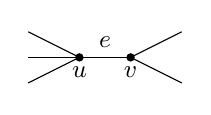
\begin{tikzpicture} [scale=.65]
    \coordinate (A) at (1, 0);
    \coordinate (B) at (2, 0);
    \coordinate (E) at (0, 0.5);
    \coordinate (F) at (0, 0);
    \coordinate (G) at (0, -0.5);
    \coordinate (H) at (3, 0.5);
    \coordinate (I) at (3, -0.5);
    \coordinate (M) at (1.5, 0);
    \draw (A) -- (B);
    \draw (A) -- (E);
    \draw (A) -- (F);
    \draw (A) -- (G);
    \draw (H) -- (B);
    \draw (I) -- (B);
    \filldraw[black] (A) circle (2pt) node[below] {\small $u$};
    \filldraw[black] (B) circle (2pt) node[below] {\small $v$};
    \draw (M) circle (0pt) node[above] {\small $e$};
  \end{tikzpicture}
\\
$G$         } \qquad
 \parbox[b]{0.8in}{   \centering
  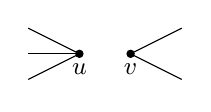
\begin{tikzpicture} [scale=.65]
     \coordinate (A) at (1, 0);
     \coordinate (B) at (2, 0);
     \coordinate (E) at (0, 0.5);
     \coordinate (F) at (0, 0);
     \coordinate (G) at (0, -0.5);
     \coordinate (H) at (3, 0.5);
     \coordinate (I) at (3, -0.5);
     \coordinate (M) at (1.5, 0);
     \draw (A) -- (E);
     \draw (A) -- (F);
     \draw (A) -- (G);
     \draw (H) -- (B);
     \draw (I) -- (B);
     \filldraw[black] (A) circle (2pt) node[below] {\small $u$};
     \filldraw[black] (B) circle (2pt) node[below] {\small $v$};
   \end{tikzpicture}
   \\
   $G-e$  }   \qquad
 \parbox[b]{0.8in}{   \centering
   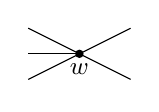
\begin{tikzpicture}  [scale=.65]
     \coordinate (A) at (1, 0);
     \coordinate (E) at (0, 0.5);
     \coordinate (F) at (0, 0);
     \coordinate (G) at (0, -0.5);
     \coordinate (H) at (2, 0.5);
     \coordinate (I) at (2, -0.5);
     \coordinate (M) at (1, 0);
     \draw (A) -- (E);
     \draw (A) -- (F);
     \draw (A) -- (G);
     \draw (H) -- (A);
     \draw (I) -- (A);
     \filldraw[black] (A) circle (2pt) node[below] {\small $w$};
   \end{tikzpicture}
   \\
   $G_e$ }  \qquad
 \parbox[b]{0.8in}{   \centering
   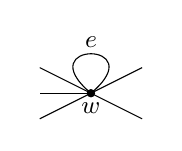
\begin{tikzpicture}[scale=.65]
    \coordinate (A) at (1, 0);
    \coordinate (E) at (0, 0.5);
    \coordinate (F) at (0, 0);
    \coordinate (G) at (0, -0.5);
    \coordinate (H) at (2, 0.5);
    \coordinate (I) at (2, -0.5);
    \coordinate (M) at (1, .7);
    \draw (A) -- (E);
    \draw (A) -- (F);
    \draw (A) -- (G);
    \draw (H) -- (A);
    \draw (I) -- (A);
    \draw (A) to[out=40,in=140,distance=1.6cm] (A);
    \filldraw[black] (A) circle (2pt) node[below] {\small $w$};
    \draw (M) circle (0pt) node[above] {\small $e$};
  \end{tikzpicture}
     \\      $G/e$    }
   \caption{Deletion, ordinary contraction, and loopy contraction of a
   non-loop edge $e$.}
   \label{fig:opers}
\end{figure}

Our main object is the multivariate invariant associated with this operation.

\begin{definition}\label{def:main}
The \emph{loopy polynomial} of a graph $G=(V,E)$ is the polynomial
\[
   \LL_G(t,\bx)=\LL_G(t,x_0,x_1,\ldots)
   \in\ZZ[t,x_0,x_1,\ldots]
\]
determined by the following properties:
\begin{enumerate}[(i)]
\item for every non-loop edge $e\in E$,
\begin{equation}\label{eq:loopy}
   \LL_G=\LL_{G/e}+t\,\LL_{G-e};
\end{equation}
\item if $G_1$ and $G_2$ are disjoint graphs, then
\[
   \LL_{G_1\sqcup G_2}=\LL_{G_1}\LL_{G_2};
\]
\item if $L_m$ denotes the graph with one vertex and $m$ loops, then
\begin{equation}\label{eq:init}
   \LL_{L_m}=x_m.
\end{equation}
\end{enumerate}
\end{definition}
In Section~\ref{sec:properties} we prove that this is well-defined and that $\LL_G$,
like the Tutte polynomial,  has a forest activity expansion.
Fix a linear order on $E(G)$ and for a component $T$ of a spanning forest $F$,
let $\eps_F(T)$ be the number of externally active
edges assigned to $T$ and $\ds \eps(F): = \sum_T\eps_F(T)$.  Then
\begin{equation}\label{eq:forest-intro}
   \LL_G(t,\bx)  =  \sum_{F\in\cF(G)}
t^{|E(G)|-|F|-\eps(F)}\prod_{T\in c(F)} x_{|E(T)|+\eps_F(T)}.
\end{equation}
The right-hand side is independent of the chosen order.  In particular, the component statistic
$ |E(T)|+\eps_F(T) $ contains both size and activity information.
In Section~\ref{sec:properties} we show that the ordinary Tutte polynomial
is a specialization: if $n=|V(G)|$ and $k(G)$ is the number of connected components, then
\begin{equation}\label{eq:tutte-from-L-intro}
T_G(X,Y) = (X-1)^{-k(G)}Y^{-n} \LL_G\bigl(1,(X-1)Y,(X-1)Y^2,(X-1)Y^3,\ldots\bigr).
\end{equation}
The loopy polynomial is nevertheless nonmatroidal.
For instance, it distinguishes the path $P_4$ from the star $K_{1,3}$, although both have Tutte polynomial $X^3$.
Moreover, $\LL_G$ is irreducible exactly when $G$ is connected,
and its irreducible factorization recovers the loopy polynomials of the connected components.

Comparing $\LL_G$ with classical graph polynomials
in Sections~\ref{sec:vertex-deletion} and~\ref{sec:relations},
we prove that $\LL_G$ determines Stanley's chromatic symmetric function~\cite{Sta} for all graphs and the matching polynomial for simple graphs.
%
We show that for loopless graphs $\LL_G$ satisfies the \emph{vertex-deletion identity}
\begin{equation}\label{eq:vertex-deletion-intro}
  \frac{\partial}{\partial x_0}\LL_G(t,\bx)
  =
  \sum_{v\in V(G)}t^{d(v)}\LL_{G-v}(t,\bx)
\end{equation}
which determines the degree sequence.
Its higher derivatives recover the \emph{induced edge count profile}
\[
  N_G(s,j) = |\{S\subseteq V(G):|S|=s,\ e_G(S)=j\}|,
\]
and hence the independence polynomial.
For simple graphs it also recovers the clique polynomial.


The forest activity expansion~\eqref{eq:forest-intro} connects $\LL_G$ with other classical
invariants: Tutte's universal $V$-function $\cV_G$~\cite{Tu1},
Brylawski's polychromate $\eta_G$~\cite{Bry}, Stanley's Tutte symmetric function $\XB_G$~\cite{Sta2}, and the $U$-polynomial of Noble and Welsh~\cite{NW}.
%
Wang and Sachs~\cite{WS}, and later Bollob\'{a}s, Pebody and Riordan~\cite{BPR},
gave a spanning forest expansion of $\cV_G$ with components weighted by external activity.
We prove in Section~\ref{subsec:loopy-V} that
\[
  \LL_G(1,\bx)    =    \left.   \cV_{G^\circ}(\bv)  \right|_{v_r=x_{r-1}\ (r\ge 1)},
\]
where $G^\circ$ is the graph obtained from $G$ by adding a new loop at every vertex.
%
Thus the \emph{ungraded loopy polynomial} $\LL_G(1,\bx)$ is simply the relabeled
universal $V$-function of the loop-augmented graph.
The grading adds no new information: we show in Section~\ref{sec:properties}
that $\LL_G(t,\bx)$ and $\LL_G(1,\bx)$ determine one another.

A second comparison comes from separating the two component statistics in \eqref{eq:forest-intro}.
In Section~\ref{sec:refined} we introduce the \emph{refined loopy polynomial}
\[
   \widehat{\LL}_G(\bu)
   =
   \sum_{F\in\cF(G)}
   \prod_{T\in c(F)}u_{|V(T)|,\eps_F(T)}.
 \]
 and prove that it
is related to the extended $U$-polynomial $U^\ext$ by an invertible componentwise binomial transform.
By Merino and Noble~\cite{MN}, $U^\ext$ is in turn
equivalent to the extended polychromate.
Thus $\widehat{\LL}_G$ determines the ordinary $U$-polynomial, Brylawski's polychromate, and Stanley's Tutte symmetric function; these three invariants are equivalent by~\cite{NW,Sar,MN,Nob}.
The resulting picture of dependencies is
\begin{equation}\label{eq:common-diagram-intro}
\begin{array}{ccccc}
&& U_G^{\ext}\ \longleftrightarrow\ \widehat{\LL}_G
   \ \longleftrightarrow\ \eta_G^{\ext} &&\\[2mm]
& \swarrow & \downarrow & \searrow &\\[-1mm]
U_G\ \longleftrightarrow\ \eta_G\ \longleftrightarrow\ \XB_G
& & \cV_G & & \LL_G .
\end{array}
\end{equation}
The three downward specializations retain different parts of the componentwise data: the $U$-specialization remembers component sizes and the total cyclomatic weight, the universal $V$-function remembers activity, and the loopy specialization keeps the diagonal combination $s-1+r$.

On forests all of the above invariants have the same distinguishing power.
\medskip

Because $\widehat{\LL}_G$ is equivalent to the extended $U$-polynomial, it determines the \emph{block statistics} of $G$: for every $b$, the joint
distribution of block sizes and internal edge counts over the partitions of $V(G)$ into $b$ parts (Section~\ref{subsec:block-statistics}).  Several
invariants studied independently are graded pieces of these data.
The two-block layer is Crew's generalized degree polynomial~\cite{Crew} or,
equivalently, Markstr\"om's homomorphism polynomial $P_2$~\cite{Mar} which also determines
the bivariate Ising polynomial of Andr\'en and Markstr\"om~\cite{AM} (Section~\ref{subsec:ising}).
Consequently $\widehat{\LL}_G$ determines all three.
Thus a conjecture of Crew that $U_G$ determines the generalized degree polynomial
and a problem of Markstr\"om on whether $U_G$ determines $P_2$
both follow, for simple graphs, if the ordinary $U$-polynomial determines the extended
one---the problem of Merino and Noble, discussed below. The boundary is sharp:
$\widehat{\LL}_G$ does not determine $P_3$. Also $\widehat{\LL}_G$ determines
the degree sequence of an arbitrary graph, loops included (Section~\ref{subsec:degree-loops}).

Adding loops to a graph can be viewed as weighting its vertices by nonnegative integers,
so the loopy polynomial of a looped graph serves as a vertex-weighted invariant of the underlying
loopless one and thus no separate weighted theory is needed (Section~\ref{sec:loops-weights}).
The two extremes of this operation, uniform weights and a single unit weight, differ sharply.
Adding enough loops uniformly at every vertex recovers $\widehat{\LL}_G$, so the question whether
$\LL_G$ determines  $\widehat{\LL}_G$
(Problem~\ref{prob:extended} below) becomes a question about $\LL$ alone.
Adding a single loop at a single vertex already produces data that $\widehat{\LL}_G$ does not determine.
\medskip

 These comparisons lead to our \emph{equivalence conjecture}.
 For simple graphs we expect
\begin{equation}\label{eq:main-conjecture-intro}
   \LL_G=\LL_H
   \quad\Longleftrightarrow\quad
   U_G=U_H
   \quad\Longleftrightarrow\quad
   \eta_G=\eta_H
   \quad\Longleftrightarrow\quad
   \XB_G=\XB_H.
\end{equation}
In Section~\ref{sec:tutte-symmetric} we give computer-assisted verification of this conjecture for
all simple graphs on at most eleven vertices.
We also verified that, up to eleven vertices, the ordinary and extended $U$-polynomials
have the same distinguishing power,
extending Markstr\"om's verification through ten vertices~\cite{Mar}.
The restriction to simple graphs is essential for
\eqref{eq:main-conjecture-intro}: loops already give a three-vertex
counterexample, and we exhibit a pair of loopless multigraphs on five vertices
with equal $U$-polynomials but distinct loopy and extended $U$-polynomials.
The latter solves the open problem of Merino and Noble~\cite{MN}.  By contrast, in
all $48\,229\,871$ connected loopless multigraphs tested, equality of loopy polynomials
also forced equality of refined loopy polynomials.  Whether this implication
holds in general is our Problem~\ref{prob:extended}.

We also present in  Section~\ref{sec:structural-evidence} four structural
results bearing on the conjecture:
the collision classes are closed under complementation and under joins,
which accounts for much of the shape of the census;
the implication $U_G=U_H \Leftarrow \LL_G=\LL_H$
is restated as a compatibility problem for block transforms;
the unicyclic case is reduced to an injectivity problem for a specialization
of the rooted $U$-polynomial~\cite{ADZ}, and settled unconditionally when the cycle is long relative to the graph;
and the normalized loopy polynomial satisfies the same triangular modular four-term
relation~\eqref{eq:normalized-4term} as Stanley's Tutte symmetric function~\cite{OS}.

Our second main contribution, presented in Section~\ref{sec:polyhedral}, is polyhedral.
For $S\subseteq V(G)$ let $\kp_G(S)$ be the number
of edges incident to at least one vertex of $S$ and consider the \emph{score polytope}
\[
   P_G=
   \{\ba\in\RR_{\ge 0}^{V(G)}:\ba(S)\le\kp_G(S)
      \text{ for every }S\subseteq V(G)\},
\]
 the independence polytope of the score polymatroid of~\cite{KNSV}.

We show that loopy deletion-contraction has a direct geometric realization as an operation on
$P_G$. For an oriented non-loop edge $e$, deletion is a translate of $P_{G-e}$ inside $P_G$,
and loopy contraction is the subcomplex swept
out by the upper endpoints of the fibers of the projection $P_G\to P_{G/e}$.
Thus the recursion~\eqref{eq:loopy} defining $\LL_G$ has two realizations: on polynomials and on polytopes.
Iterating the one-step
construction produces pairwise disjoint forest-indexed geometric parking complexes $\fC_F\subseteq P_G$,
piecewise integral-affinely parametrized by the boxes
\[
   \prod_{T\in c(F)}[0,|E(T)|+\eps_F(T)].
\]
Their lattice points partition $P_G\cap\ZZ^{V(G)}$, while the complement of their union is lattice-free.
Their generating function
\[
   \sum_{\ba\in P_G\cap\ZZ^{V(G)}}q^{|\ba|}
   =
   \LL_G(q,1,1+q,1+q+q^2,\ldots),
\]
is the external bizonotopal Hilbert series of~\cite{KNSV}.  More importantly, it explains the component weight in~\eqref{eq:forest-intro}: the number
$|E(T)|+\eps_F(T)$ attached to a forest component is the length of an actual interval factor.
This connects the two halves of the paper.
The combination of size and activity that
separates $\LL_G$ from the other specializations of the common refinement is exactly the combination that carries polyhedral meaning.
The same submodular function $\kp_G$ governs
both sides: it is the exponent in the higher vertex-deletion identity of
Section~\ref{sec:vertex-deletion} and the rank function defining $P_G$.

In Section~\ref{sec:outlook} we discuss further questions.
The computational method is described in
Appendix~\ref{sec:the-computation}.

\paragraph{Conventions and notation.}
Throughout, by ``graph'' we understand a finite undirected multigraph.
Loops and multiple edges are allowed unless explicitly stated otherwise, and multiple edges are regarded as distinct.
We write $V(G)$ and $E(G)$ for the vertex and edge sets, $n(G)$ for the number of vertices,
$m(G)$ for the number of edges (with loops and parallel copies counted with multiplicity),
$c(G)$ for the set of connected components, and $k(G)$ for the number of connected components.
The rank and cyclomatic number (the first Betti number) are
\[
   r(G)=n(G)-k(G), \qquad \nu(G)=m(G)-r(G)=m(G)-n(G)+k(G).
\]
When the graph is fixed we usually abbreviate these to $n, m, k, r, \nu$.
For $v\in V(G)$ let $\ell_G(v)$ be the number of loops at $v$, and let $\ell(G)$
be the total number of loops of $G$.  For $S\subseteq V(G)$ we write $e_G(S)$ for
the number of edges of $G$ induced on $S$, that is, with both endpoints in $S$,
and $\kp_G(S)$ for the number of edges having at least one endpoint in $S$.

For $e\in E(G)$, we write $e=uv$ to indicate that $e$ has endpoints $u,v\in V(G)$.
The notation $G-e$ means deletion of that particular edge. If $e$ is a non-loop edge,
$G/e$ denotes its loopy contraction, whereas $G_e$ denotes ordinary contraction.
For a vertex $v$, $G-v$ denotes \emph{vertex deletion}: the graph obtained by removing $v$
together with all edges incident to $v$.  We write $\overline G$ for the complement of a simple graph $G$.
If $e_1,\ldots,e_k$ are specified edges, the notation
\[
   G+\{e_1,\ldots,e_k\}
\]
means the graph obtained from $G$ by adjoining these edges as new copies.
Thus, if an edge with the same endpoints is already present in $G$, it is not identified with the new edge.
On edge sets the operation is understood as multiset union.  The same convention applies
when several of the added edges have the same endpoints.

A \emph{spanning forest} of $G$ means any spanning acyclic subgraph, not necessarily maximal.
We identify a spanning forest with its edge set and write $\cF(G)$ for the set of spanning
forests and $c(F)$ for the set of connected components of $(V(G),F)$.  Loops are never edges of a forest.

Whenever activity is used, the edge set is equipped with a linear order and we
use the least-edge convention.  For a spanning forest $F$ and an edge $e\notin
F$, we call $e$ \emph{externally active} relative to $F$ if either $e$ is a
loop, or the endpoints of $e$ lie in the same component of $F$ and $e$ is the
least edge of the unique cycle contained in $F\cup\{e\}$.  Thus a loop is a
one-edge cycle and is externally active relative to every spanning forest,
whereas an edge joining two distinct components of $F$ closes no cycle and is
never active.  An externally active edge is \emph{assigned} to the component
of $F$ containing its endpoints.  For $T\in c(F)$ we write $\eps_F(T)$
for the number of externally active edges assigned to $T$, and
\[
   \eps(F)=\sum_{T\in c(F)}\eps_F(T).
\]
When the ambient graph has to be indicated we write $\eps_G(F)$ for the external activity
of $F$ computed in $G$.  The \emph{weight} $\wt_G(F)$ of a spanning forest
is defined in~\eqref{eq:forest-weight}. It is the contribution of $F$ to the forest expansion of $\LL_G$.

For graph invariants $P$ and $Q$ on a class $\cG$, we say that they have
the same distinguishing power, or induce the same fibers, if $P_G=P_H$
if and only if $Q_G=Q_H$ for all $G,H\in\cG$.  When an explicit invertible specialization or
coefficient transformation is available, we state this stronger relation separately.

We write $\RR^I$ for the real vector space with coordinates indexed by $I$, and $\ZZ^I \subseteq \RR^I$
for its integer lattice. Thus $\ZZ^{V}$ has coordinates labeled by the vertices of $G$,
and coordinates of $\RR^{c(F)}$ are  labeled by the components of a spanning forest $F$.

For a vector $\ba=(a_v)_{v\in V}$ and $S\subseteq V$, we write
$\ba(S):=\sum_{v\in S}a_v$ and $|\ba|:=\ba(V)=\sum_{v\in V}a_v$.
For a polynomial or formal series $P$ and a monomial $M$, the standard notation
$[M]P$ denotes the coefficient of $M$ in $P$.  We write $p_k$ for the $k$th power-sum symmetric function.

Below $T_G$ denotes the ordinary Tutte polynomial,
$\cV_G$ Tutte's 1947 universal $V$-function, $U_G$ the Noble--Welsh $U$-polynomial,
and $U_G^{\ext}$ its extended version.
We use $\eta_G$ and $\eta_G^{\ext}$ for the ordinary and extended polychromates,
$X_G$ for Stanley's chromatic symmetric function, and $\XB_G$ for Stanley's Tutte symmetric function.
The refined loopy polynomial introduced in Section~\ref{sec:refined} is denoted $\widehat{\LL}_G$.
Finally, $\cA_G^e,\cA_G^c$ denote the external and central graphical zonotopal algebras,
and $\BZ_G^e,\BZ_G^c$ the external and central bizonotopal algebras of~\cite{KNSV}.

Substitutions involving negative powers of $t$ are understood in the Laurent polynomial ring.
In every formula with such a substitution, the indicated overall power of $t$ restores an ordinary polynomial.


\section{The loopy polynomial: definition and basic properties}\label{sec:properties}

\subsection{Loopy deletion-contraction and well-definedness}\label{subsec:well-definedness}

The loopy deletion-contraction relation~\eqref{eq:loopy} gives a recursive
procedure for computing $\LL_G$: choose a non-loop edge, apply
\eqref{eq:loopy}, and continue until all remaining edges are loops.  The same
loopy deletion-contraction recurrence occurs in~\cite[Theorem~3.5]{KNSV} for
the Hilbert series $h_G^{(r)}(t)$ of the bizonotopal algebras, for every
$r\ge 0$.  Here the variables $x_0,x_1,\ldots$ are independent, so we first
verify directly that the resulting multivariate recursion is well defined.

\begin{proposition}\label{prop:well-def}
The polynomial obtained from Definition~\ref{def:main} is independent of all
choices made in the loopy deletion-contraction recursion.
\end{proposition}

\begin{proof}
We use induction on the number $N$ of non-loop edges.  There is nothing to
prove for $N=0$.  Suppose $N>0$, and let $e$ and $f$ be two non-loop edges
which could be chosen as the edge of the recursion.

Assume first that $e$ and $f$ are not parallel.  After applying loopy
deletion-contraction first to $e$ and then to $f$, we obtain
\[
 \LL_{(G/e)/f}
 +t\LL_{(G/e)-f}
 +t\LL_{(G-e)/f}
 +t^2\LL_{G-e-f}.
\]
Applying the recursion in the opposite order gives
\[
 \LL_{(G/f)/e}
 +t\LL_{(G/f)-e}
 +t\LL_{(G-f)/e}
 +t^2\LL_{G-e-f}.
\]
The four graphs in the first expression are canonically isomorphic, respectively, to the four graphs in the second expression.  Indeed, deletion and loopy contraction commute for distinct non-parallel edges, and the two
loopy contractions identify the same vertices and retain both contracted edges as loops.
All terms occurring after these first two operations have fewer than $N$ non-loop edges, so the induction hypothesis applies to their further evaluation.

Suppose now that $e$ and $f$ are parallel.  Loopy contraction of either one turns the other into a loop, so it is no longer processed, and loops are never chosen by the recursion.  Expanding first in $e$ gives
\[
 \LL_{G/e}
 +t\LL_{(G-e)/f}
 +t^2\LL_{G-e-f},
\]
whereas expanding first in $f$ gives
\[
 \LL_{G/f}
 +t\LL_{(G-f)/e}
 +t^2\LL_{G-e-f}.
\]
Again the corresponding graphs are canonically isomorphic: $G/e\cong G/f$ and $(G-e)/f\cong(G-f)/e$.
The induction hypothesis completes the argument.
\end{proof}
\subsection{The forest expansion and Tutte specialization} \label{subsec:forest-expansion}

We next give a spanning-forest description of $\LL_G$.  Recall that the activity expansion of Tutte polynomial
is indexed by maximal spanning forests and records internal and external activity globally (see for example~\cite{Tu2,EM}).
The expansion~\eqref{eq:forests} below instead runs over all spanning forests and distributes
external activity among their connected components.
Fix a linear order on $E(G)$. Recall that an edge $e\in E(G)\setminus F$ is called \emph{externally active}
relative to the spanning forest $F$ if it is a loop, or if its endpoints lie
in the same component of $F$ and $e$ is the least edge of the unique cycle in
$F\cup\{e\}$.  In that case $e$ is assigned to the component containing its endpoints.
Denote by $\EA(F)$ the set of all externally active edges of $F$, by $\eps_F(T)$ the number of
externally active edges assigned to $T\in c(F)$ and by
$\ds \eps(F)=\sum_{T\in c(F)}\eps_F(T)=|\EA(F)|  $
their total.  Two features distinguish our expansion from the classical convention: it
runs over \emph{all} spanning forests, not only the maximal ones, and the activity is recorded
per component rather than globally.
\medskip

For a spanning forest $F$ of a graph $G$ with ordered $E(G)$ we write
\begin{equation}\label{eq:forest-weight}
 \wt_G(F)  :=  t^{|E(G)|-|F|-\eps(F)}
 \prod_{T\in c(F)} x_{|E(T)|+\eps_F(T)}
\end{equation}
for the \emph{weight} of $F$ in $G$. Here $|E(T)|=|V(T)|-1$, since the components of a forest are trees.

\begin{theorem}[The forest expansion]\label{thm:forests-sum}
For every graph $G$ and every ordering of $E(G)$,
\begin{equation}\label{eq:forests}
  \LL_G(t,\bx) = \sum_{F\in\cF(G)}  t^{|E(G)|-|F|-\eps(F)}
  \prod_{T\in c(F)}  x_{|E(T)|+\eps_F(T)}.
\end{equation}
That is, $\ds \LL_G=\sum_{F\in\cF(G)}\wt_G(F)$.
In particular, the right-hand side is independent of the edge order.
\end{theorem}

\begin{proof}
 Let $\Phi_G$ denote the right-hand side of~\eqref{eq:forests}, and let $e$ be the largest non-loop edge of $G$.
 We partition the spanning forests of $G$ according to whether they contain $e$.

Suppose first that $e\notin F$.  Then $F$ is a spanning forest of $G-e$.
Moreover, $e$ is not externally active relative to $F$: if its endpoints lie
in the same component of $F$, the cycle in $F\cup\{e\}$ contains another
edge, and $e$, being the largest edge, cannot be its least edge.
The external activities and their component assignments are therefore exactly
the same in $G$ and in $G-e$.  Since
$|E(G)|=|E(G-e)|+1$, the forests omitting $e$ contribute  $ t\,\Phi_{G-e}$.

Now suppose that $e\in F$.  Contracting $e$ gives a bijection
\[
   F\longmapsto F/e:=F\setminus\{e\}
\]
from spanning forests of $G$ containing $e$ to spanning forests of $G/e$.
Recall that loopy contraction retains $e$ as a loop.  Thus $e$ is externally
active in $G/e$ relative to $F/e$.

All other external activities are unchanged.  Indeed, if $f\in E(G)\setminus F$, then its fundamental cycle is either unaffected by the
contraction or is obtained by deleting $e$ from the corresponding cycle in
$G$.  Since $e$ is the largest edge, deleting it does not change whether
$f$ is the least edge of that cycle.  In particular, if $f$ is parallel to
$e$, then $f<e$ and $f$ is active both before contraction, as the least edge
of the two-edge cycle, and after contraction, when it becomes a loop.
Component assignments are also unchanged.

Let $T$ be the component of $F$ containing $e$.  In $F/e$ it is replaced by a component $T/e$ with
\[
   |V(T/e)|=|V(T)|-1,
   \qquad
   \eps_{F/e}(T/e)=\eps_F(T)+1.
\]
Hence
\[
 |V(T/e)|-1+\eps_{F/e}(T/e)  =  |E(T)|+\eps_F(T),
\quad |F/e|=|F|-1, \quad \text{and}  \quad  \eps(F/e)=\eps(F)+1,
\]
while $|E(G/e)|=|E(G)|$.  Therefore the power of $t$ is unchanged:
\[
 |E(G/e)|-|F/e|-\eps(F/e)  =  |E(G)|-|F|-\eps(F).
\]
It follows that the forests containing $e$ contribute exactly $\Phi_{G/e}$ giving
$ \Phi_G=\Phi_{G/e}+t\Phi_{G-e}. $

Finally, if $G$ has only loop edges, each of them is externally active for the unique spanning forest, so
\[
   \Phi_G=\prod_{v\in V(G)}x_{\ell_G(v)},
\]
agreeing with the initial
conditions and multiplicativity in Definition~\ref{def:main}.  By
Proposition~\ref{prop:well-def}, $\Phi_G=\LL_G$.
\end{proof}

\begin{remark}\label{rem:V-forest-history}
A closely related componentwise spanning-forest activity expansion occurs in
the theory of Tutte's universal $V$-function.  Wang and Sachs~\cite{WS}
expressed the general $V$-function as a sum over spanning forests in which
each component is weighted by the number of externally active edges associated
with it, see also Bollob\'as, Pebody and Riordan~\cite{BPR}.
In Section~\ref{sec:relations} we make this connection precise.  If $G^\circ$ is
obtained from $G$ by adding one loop at every vertex, then the specialization at $t=1$ of~\eqref{eq:forests} is exactly the corresponding universal $V$-function expansion for $G^\circ$, after a relabeling of variables.  Thus
Theorem~\ref{thm:forests-sum} may also be viewed as the graded loopy form of
this classical expansion.
\end{remark}

Theorem~\ref{thm:forests-sum} represents $\LL_G$ as a sum over spanning forests, whereas the
classical invariants with which we compare it in
Sections~\ref{sec:relations} and~\ref{sec:refined} --- the $U$-polynomial,
the polychromate and the chromatic symmetric function --- are sums over arbitrary subsets of $E(G)$.
These two summations are reconciled by a
decomposition of the Boolean lattice of edge sets, in which each spanning
forest defines an interval of subsets having the same components as itself.
We will use it below, in the proof
that the Tutte polynomial is a specialization of $\LL_G$, and three more times in Sections~\ref{sec:relations} and~\ref{sec:refined}.
On each occasion it is what turns a sum over
subsets into a sum over forests.
For a spanning forest $F$ we denote by $\EA(F)$ the set of its externally active edges.

\begin{lemma}\label{lem:activity-intervals}
For any edge order the Boolean lattice $2^{E(G)}$ is the disjoint union of the intervals
\begin{equation}\label{eq:activity-intervals}
  [F,F\cup\operatorname{EA}(F)]
  :=
  \{F\cup J:J\subseteq\operatorname{EA}(F)\},
  \qquad F\in\mathcal F(G).
\end{equation}
\end{lemma}

\begin{proof}
  Use induction on the number of non-loop edges.  A loop is externally active for every forest and may be either present or absent independently,
 so loops cause no difficulty.  Let $e$ be the largest non-loop edge.  Since our active edge is the least edge in its cycle, $e$ is never externally active.
The subsets not containing $e$ are partitioned by the intervals for $G-e$.
The subsets containing $e$ correspond, after contraction of $e$, to the subsets of $G_e$, and forests containing $e$ correspond to forests of $G_e$.
Because $e$ is largest, contraction preserves the external activity of every other edge.
The induction hypothesis therefore gives the required disjoint partition in both classes.
\end{proof}

The forest expansion~\eqref{eq:forests} also gives a direct specialization of $\LL_G$ to the Tutte polynomial $T_G$.
%
We use the rank-nullity form of the Tutte polynomial,  see~\cite{Tu2,EM}. Let
$r(A)=n(G)-k\bigl(V(G),A\bigr)$ be the rank of a
spanning subgraph with edge set $A\subseteq E(G)$.
Then
\begin{equation}\label{eq:tutte-rank-nullity}
  T_G(X,Y)  =   \sum_{A\subseteq E(G)}
  (X-1)^{\,r(E)-r(A)}\,(Y-1)^{\,|A|-r(A)} .
\end{equation}
This is multiplicative over connected components, and a loop contributes a factor $Y$.


First we use Lemma~\ref{lem:activity-intervals} to write $T_G$ as a sum over \emph{all} spanning forests, weighted by external activity.

\begin{corollary}[All-forest form of the Tutte polynomial]
\label{cor:tutte-all-forests}
For every graph $G$ and every ordering of $E(G)$,
\begin{equation}\label{eq:tutte-all-forests}
   (X-1)^{k}\,T_G(X,Y)
   =
   \sum_{F\in\cF(G)}(X-1)^{|c(F)|}\,Y^{\eps(F)} .
\end{equation}
\end{corollary}

\begin{proof}
  Group the summands of~\eqref{eq:tutte-rank-nullity} by the intervals of Lemma~\ref{lem:activity-intervals}.
 Let $A=F\cup S$ with $S\subseteq\EA(F)$.  An externally active edge has both endpoints in one
component of $F$, so adding the edges of $S$ merges no components and $k\bigl(V(G),A\bigr)=|c(F)|$.  Hence
\[
   r(A)=n-|c(F)|=|F|,  \qquad  |A|-r(A)=|S|,
   \qquad    r(E)-r(A)=|c(F)|-k .
\]
The interval corresponding to $F$ therefore contributes
\[
(X-1)^{\,|c(F)|-k} \sum_{S\subseteq\EA(F)}(Y-1)^{|S|}
 =(X-1)^{\,|c(F)|-k}\,Y^{\eps(F)},
\]
since $\eps(F)=|\EA(F)|$.  Summing over $F\in\cF(G)$ and multiplying by~$(X-1)^{k}$  gives~\eqref{eq:tutte-all-forests}.
\end{proof}


\begin{corollary}[Tutte specialization]\label{cor:tutte-specialization}
Let $n=|V(G)|$, $m=|E(G)|$, and $k=k(G)$.  Then
\begin{equation}\label{eq:tutte-specialization}
\LL_G\bigl(  t,(X-1)Y,(X-1)tY^2,(X-1)t^2Y^3,\ldots \bigr)
= t^m(X-1)^kY^nT_G(X,Y).
\end{equation}
In particular,
\begin{equation}\label{eq:tutte-specialization-t1}
T_G(X,Y) = (X-1)^{-k}Y^{-n}
\LL_G\bigl(1,(X-1)Y,(X-1)Y^2,\ldots\bigr).
\end{equation}
\end{corollary}

\begin{proof}
Substitute $ x_i=(X-1)t^iY^{i+1}$ in~\eqref{eq:forests}.
Then the weight~\eqref{eq:forest-weight} of a spanning forest $F$ becomes
\[
t^{m-|F|-\varepsilon(F)}  \prod_{T\in c(F)}
 \left((X-1)t^{|E(T)|+\varepsilon_F(T)}
 Y^{|V(T)|+\varepsilon_F(T)}\right)
=  t^m(X-1)^{|c(F)|}Y^{n+\varepsilon(F)}
\]
because $\ds  \sum_{T\in c(F)}|V(T)|=n $ and $\ds  \sum_{T\in c(F)}(|V(T)|-1)=|F| $.

Now summing over $F$  and applying  Corollary~\ref{cor:tutte-all-forests} we obtain~\eqref{eq:tutte-specialization}.
%
Setting $t=1$ gives~ \eqref{eq:tutte-specialization-t1}.
\end{proof}

The simplest special case of Theorem~\ref{thm:forests-sum} is worth recording separately.

\begin{corollary}\label{cor:forest-L}
  If $G$ is a forest, then
  \begin{equation}
    \label{eq:loopy-forests}
    \LL_G(t,\bx)  =  \sum_{A\subseteq E(G)}
    t^{|E(G)|-|A|}  \prod_{T\in c(A)}x_{|V(T)|-1}.
  \end{equation}
\end{corollary}

\begin{proof}
If $G$ is a forest and $A\subseteq E(G)$, then every edge of   $E(G)\setminus A$ has its endpoints in different components of $A$.
  Thus there are no externally active edges, and the result follows from Theorem~\ref{thm:forests-sum}.
\end{proof}


\subsection{Degree, extremal terms, and multiplicativity}\label{sec:corols}

We collect several immediate consequences of the forest expansion.  For a
monomial in the variables $\bx$, its \emph{ordinary $\bx$-degree} means the
total degree obtained by assigning degree $1$ to every $x_i$.

\begin{corollary}\label{th:cor}
  Let $n=|V(G)|$, $m=|E(G)|$, and
let $ \nu(G)=m-n+k(G)$ be the cyclomatic number of $G$.
Denote by $\cA_G^e, \ \cA_G^c, \ \BZ_G^e$ and $\BZ_G^c$  the external and central graphical zonotopal algebras (see~\cite{PS,HR}) and
the external and central bizonotopal algebras of~\cite{KNSV} respectively.
\begin{enumerate}[(1)]
\item If $G$ is loopless, then the unique term of $\LL_G$ of $x_0$-degree $n$ is \   $ t^m x_0^n$.

\item If $G$ is simple, then
\[
   [x_0^{n-2}x_1]\,\LL_G(t,\bx)=m\,t^{m-1}.
\]

\item With a grading
  $ \deg t=1, \ \deg x_i=i,$
the polynomial $\LL_G$ is homogeneous of degree $m$.  In other words,
\begin{equation}\label{eq:scaling-L}
   \LL_G(t,\bx)  =
  t^m\LL_G\bigl(1,x_0,t^{-1}x_1,t^{-2}x_2,\ldots\bigr).
\end{equation}

\item The number of edges $m(G)$ is recoverable from the ungraded polynomial
  $\LL_G(1,\bx)$  as
the maximum weighted $\bx$-degree with $\deg x_i=i$.  Thus polynomials  $\LL_G(t,\bx)$ and $\LL_G(1,\bx)$ determine one another.

\item The maximum  $\bx$-degree of a monomial occurring in $\LL_G$ is $n$, and the minimum is $k$.
 In particular, $\LL_G$ determines $n$ and $k$ and detects whether $G$ is connected.

\item The Hilbert series of $\cA_G^e$ is
\[
 \Hil(\cA_G^e;t)  = \LL_G(t,1,1,\ldots)  =
 t^{\nu(G)}T_G(1+t,t^{-1}).
\]

\item If $G$ is connected and $\LL_G^{(1)}$ is the part of $\LL_G$ of ordinary $\bx$-degree $1$,
  then the Hilbert series of $\cA_G^c$ is
\[
 \Hil(\cA_G^c;t)
 =
 \left.\LL_G^{(1)}(t,\bx)\right|_{x_i=1}
 =
 t^{\nu(G)}T_G(1,t^{-1}).
\]

\item The Hilbert series of $\BZ_G^e$ is obtained by the substitution $x_i\longmapsto 1+t+\cdots+t^i$, that is \begin{equation}\label{eq:external-biz-specialization}
 \Hil(\BZ_G^e;t)
 =
 \LL_G\bigl(t,1,1+t,1+t+t^2,\ldots\bigr).
\end{equation}

\item The Hilbert series of $\BZ_G^c$ is obtained by
\   $  x_0\longmapsto0, \quad
  x_i\longmapsto1+t+\cdots+t^{i-1} \quad(i\ge 1)
$
, that is
\begin{equation}\label{eq:central-biz-specialization}
 \Hil(\BZ_G^c;t)
 =
 \LL_G\bigl(t,0,1,1+t,1+t+t^2,\ldots\bigr).
\end{equation}
\end{enumerate}
\end{corollary}

\begin{proof}
 For~(1), the empty forest has $n$ singleton components and, since $G$ is loopless, no external activity.  Thus it contributes $t^m x_0^n$ to~\eqref{eq:forests}.  Every nonempty
forest has a nonsingleton component and therefore has smaller $x_0$-degree.

For~(2), a term $x_0^{n-2}x_1$ can only come from a spanning forest consisting
of one edge and $n-2$ isolated vertices.  Since $G$ is simple, such a forest
has no external activity.  There are exactly $m$ choices of the edge, each
contributing $t^{m-1}x_0^{n-2}x_1$.

For~(3), every term indexed by a spanning forest $F$ has total weighted degree
\[
|E(G)|-|F|-\eps(F)  +\sum_{T\in c(F)}
 \bigl(|E(T)|+\eps_F(T)\bigr)
= m-|F|-\eps(F)+|F|+\eps(F) = m.
\]
Equivalently, the weighted $\bx$-degree of the forest monomial is
$|F|+\eps(F)$, which gives~\eqref{eq:scaling-L} term by term.

For~(4), it remains to see that $m$ itself is recoverable from
$\LL_G(1,\bx)$.
Construct a maximal spanning forest greedily by processing the non-loop edges
from largest to smallest and adding an edge whenever it does not create a
cycle.  Any omitted non-loop edge is then the least edge of its fundamental cycle, and any loop is externally active.  Thus every edge outside this
 forest is externally active and so
  $ |F|+\eps(F)=m.$
Thus a monomial of weighted $\bx$-degree $m$ occurs in $\LL_G(1,\bx)$.
All forest monomials have weighted degree at most $m$, so $m$ is exactly the
maximum such degree.  The scaling identity therefore reconstructs the full
polynomial from its specialization at $t=1$.

For~(5), the ordinary $\bx$-degree of the term associated with $F$ is
$|c(F)|$.  Its largest possible value is $n$, attained only by the empty
forest, while its smallest possible value is $k(G)$, attained by every maximal
spanning forest.

For~(6), setting all $x_i=1$ in~\eqref{eq:forests} gives
\[
   \sum_{F\in\cF(G)}
   t^{m-|F|-\eps(F)},
\]
which is the standard activity expression for the external zonotopal Hilbert
series~see~\cite{PSS,HR}, equivalently
\[
   t^{m-r(G)}T_G(1+t,t^{-1}).
\]

For~(7), when $G$ is connected, the terms of ordinary $\bx$-degree $1$ are
precisely those indexed by spanning trees.  Setting the remaining $x_i$ equal
to $1$ gives the standard activity expression
\[
   t^{m-n+1}T_G(1,t^{-1})
\]
for the central zonotopal Hilbert series, see~\cite{PS,HR}.

Finally,~(8) and~(9) follow from \cite[Theorem~3.6]{KNSV}.  The central and external bizonotopal Hilbert
series satisfy the same loopy deletion-contraction recurrence and multiplicativity as $\LL_G$,
while on the one-vertex graph $L_i$ with $i$ loops their initial values are, respectively,
\[
   1+t+\cdots+t^{i-1}
   \qquad\text{and}\qquad
   1+t+\cdots+t^i.
\]
The substitutions in~\eqref{eq:central-biz-specialization} and
\eqref{eq:external-biz-specialization} therefore give exactly these Hilbert
series.
\end{proof}

The extremal parts of the forest expansion record a little more
of the elementary structure of the graph than the preceding corollary makes
explicit.

\begin{proposition}[Extremal terms]\label{prop:extremal-terms}
  Let $m_i$ be the edge number of the $i$th connected component of $G$.  Then
\begin{equation}\label{eq:L-at-zero-components}
   \LL_G(0,\bx)=\prod_{i=1}^{k}x_{m_i}.
\end{equation}
Moreover, the unique term of the maximal $\bx$-degree $n(G)$ is
\begin{equation}\label{eq:max-x-degree-term}
   t^{m(G)-\ell(G)}\prod_{v\in V(G)}x_{\ell_G(v)}.
\end{equation}
Thus $\LL_G$ determines the order $n$ and size $m$ of $G$, the number  of components $k$, the rank $r$, the multiset of edge counts
$\{m(G_i)\}_{i=1}^k$, and the multiset
$\{\ell_G(v):v\in V(G)\}$ of loop multiplicities at the vertices.
\end{proposition}

\begin{proof}
Suppose first that $G$ is connected and has $m$ edges.  At $t=0$ the deletion
term in loopy deletion-contraction disappears.  Contracting the non-loop
edges successively therefore reduces $G$ to the one-vertex graph $L_m$ and
gives $\LL_G(0,\bx)=x_m$.  Applying multiplicativity to the connected
components gives~\eqref{eq:L-at-zero-components}.

For the second assertion notice that a forest term has ordinary $\bx$-degree equal to
its number of components.  Degree $n(G)$ can therefore occur only for the empty forest.
Relative to the empty forest every loop is externally active and is assigned to its vertex, while no non-loop edge is externally active.
Therefore the empty forest contributes exactly
\[
   t^{m(G)-\ell(G)}\prod_{v\in V(G)}x_{\ell_G(v)},
\]
and no other forest contributes in that degree.  The stated elementary data
are now read from~\eqref{eq:L-at-zero-components},
\eqref{eq:max-x-degree-term}, and Corollary~\ref{th:cor}(3)--(4).
\end{proof}

The next result, besides being a useful structural fact in its own right,  will
also be needed in Section~\ref{sec:tutte-symmetric}, where it allows the comparison of multiplicative invariants to be reduced to connected graphs.

\begin{proposition}[Connectedness and irreducibility]
\label{prop:L-irreducible}
A graph $G$ is connected if and only if $\LL_G(t,\bx)$ is irreducible in
$\ZZ[t,x_0,x_1,\ldots]$.
\end{proposition}

\begin{proof}
If $G$ is disconnected, multiplicativity gives a nontrivial factorization of
$\LL_G$ into the loopy polynomials of its connected components.

Conversely, suppose that $G$ is connected and let $m=m(G)$.  If $m=0$, then
$G$ is a single isolated vertex and $\LL_G=x_0$.  Assume $m>0$.  By
Proposition~\ref{prop:extremal-terms},
\[
   \LL_G(0,\bx)=x_m.
\]
By Corollary~\ref{th:cor}(3), $\LL_G$ is homogeneous of weighted degree $m$
for $\deg t=1$ and $\deg x_i=i$.
So no variable $x_i$ with $i>m$ occurs,
and any monomial containing $x_m$ can contain no positive power of $t$ and no
$x_i$ with $i>0$ other than $x_m$.  A factor $x_0^j$ is not excluded by
homogeneity, since $\deg x_0=0$, but the specialization at $t=0$ rules it out:
it shows that the only such monomial is $x_m$ itself, with coefficient $1$.  Thus
\begin{equation}\label{eq:connected-monic-form}
   \LL_G=x_m+Q(t,x_0,\ldots,x_{m-1}).
\end{equation}
Regarded as a polynomial in $x_m$ over
$R=\ZZ[t,x_0,\ldots,x_{m-1}]$, it is therefore monic of degree one.
If $\LL_G=AB$, one factor, say $A$, is independent of $x_m$.  Comparing the
coefficients of $x_m$ gives $A\,[x_m]B=1$ in $R$.  Hence $A$ is a unit, so
$\LL_G$ is irreducible.
\end{proof}

\begin{corollary}[Component factorization]\label{cor:L-component-factorization}
If  $G_1,\ldots,G_k$ are the connected components of $G$, then
\[
   \LL_G=\prod_{i=1}^k\LL_{G_i}
\]
is the irreducible factorization of $\LL_G$, up to the order of the factors.
In particular, $\LL_G$ determines the multiset
$\{\LL_{G_1},\ldots,\LL_{G_k}\}$ and hence the multisets of the orders and
sizes of the connected components, with the corresponding loop data from
Proposition~\ref{prop:extremal-terms}.
\end{corollary}

\begin{proof}
Each factor is irreducible by Proposition~\ref{prop:L-irreducible}.  Since
only finitely many variables occur, uniqueness of factorization in the ordinary finite polynomial ring containing $\LL_G$ proves the claim.
\end{proof}

\subsection{The \texorpdfstring{$4$}{4}-term relation and  multistars}
\label{sec:4-terms}

\subsubsection{The \texorpdfstring{$4$}{4}-term relation}
\label{subsubsec:four-term}
Let $u,v,w$ be three distinct vertices and write
\[
   e_1=uv,    \qquad    e_2=vw,    \qquad    e_3=uw.
\]
Recall the convention that
$G+\{e_1,\ldots,e_s\}$ means that new copies of the indicated edges are
adjoined, even if edges with the same endpoints are already present in $G$.

\begin{figure}[ht]
\centering
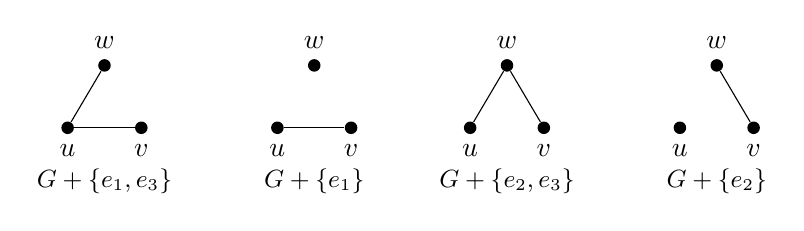
\begin{tikzpicture}[scale=.72,
  vertex/.style={circle,fill=black,inner sep=1.6pt}]

\begin{scope}[xshift=0cm]
 \node[vertex,label=below:$u$] (u) at (0,0) {};
 \node[vertex,label=below:$v$] (v) at (1.3,0) {};
 \node[vertex,label=above:$w$] (w) at (.65,1.1) {};
 \draw (u)--(v);
 \draw (u)--(w);
 \node at (.65,-.95) {\small $G+\{e_1,e_3\}$};
\end{scope}

\begin{scope}[xshift=3.7cm]
 \node[vertex,label=below:$u$] (u) at (0,0) {};
 \node[vertex,label=below:$v$] (v) at (1.3,0) {};
 \node[vertex,label=above:$w$] (w) at (.65,1.1) {};
 \draw (u)--(v);
 \node at (.65,-.95) {\small $G+\{e_1\}$};
\end{scope}

\begin{scope}[xshift=7.1cm]
 \node[vertex,label=below:$u$] (u) at (0,0) {};
 \node[vertex,label=below:$v$] (v) at (1.3,0) {};
 \node[vertex,label=above:$w$] (w) at (.65,1.1) {};
 \draw (v)--(w);
 \draw (u)--(w);
 \node at (.65,-.95) {\small $G+\{e_2,e_3\}$};
\end{scope}

\begin{scope}[xshift=10.8cm]
 \node[vertex,label=below:$u$] (u) at (0,0) {};
 \node[vertex,label=below:$v$] (v) at (1.3,0) {};
 \node[vertex,label=above:$w$] (w) at (.65,1.1) {};
 \draw (v)--(w);
 \node at (.65,-.95) {\small $G+\{e_2\}$};
\end{scope}

\end{tikzpicture}
\caption{The four local edge configurations in
Theorem~\ref{thm:4term}.  The common graph $G$ is suppressed.}
\label{fig:4term}
\end{figure}

\begin{theorem}\label{thm:4term}
For the four graphs shown in Figure~\ref{fig:4term} we have
\begin{equation}\label{eq:4term}
\LL_{G+\{e_1,e_3\}}-t\,\LL_{G+\{e_1\}}
=
\LL_{G+\{e_2,e_3\}}-t\,\LL_{G+\{e_2\}}.
\end{equation}
\end{theorem}

\begin{proof}
Apply loopy deletion-contraction to the newly added copy of $e_3$ in
$G+\{e_1,e_3\}$.  This gives
\[
\LL_{G+\{e_1,e_3\}}-t\,\LL_{G+\{e_1\}}
=
\LL_{(G+\{e_1,e_3\})/e_3}.
\]
Similarly,
\[
\LL_{G+\{e_2,e_3\}}-t\,\LL_{G+\{e_2\}}
=
\LL_{(G+\{e_2,e_3\})/e_3}.
\]
After contracting $e_3=uw$, the vertices $u$ and $w$ are identified.
Thus the new edge $e_1=uv$ in the first graph and the new edge
$e_2=vw$ in the second become corresponding edges between the
merged vertex and $v$, while $e_3$ becomes a loop at the merged vertex.
Edges already in $G$ are transformed identically.  So
\[
   (G+\{e_1,e_3\})/e_3
   \cong
   (G+\{e_2,e_3\})/e_3,
\]
which proves~\eqref{eq:4term}.
\end{proof}

It is useful to record the normalized form of the relation~\eqref{eq:4term}.  Define
\[
   \overline{\LL}_G:=t^{-|E(G)|}\LL_G.
\]
Since the four graphs in~\eqref{eq:4term} differ from $G$ by one or two
new edges, Theorem~\ref{thm:4term} is equivalent to
\begin{equation}\label{eq:normalized-4term}
\overline{\LL}_{G+\{e_1,e_3\}}
-\overline{\LL}_{G+\{e_1\}}
=
\overline{\LL}_{G+\{e_2,e_3\}}
-\overline{\LL}_{G+\{e_2\}}.
\end{equation}
This is the triangular modular relation of Orellana and Scott~\cite{OS},
the relation satisfied also by the chromatic and Tutte symmetric functions.  We return to this comparison in
Section~\ref{sec:tutte-symmetric}.

\begin{remark}\label{rem:vassiliev-4term}
The $4$-term relation of Theorem~\ref{thm:4term} should not be confused with
a different $4$-term relation on graphs arising from the theory of Vassiliev knot invariants, see~\cite{Li,La}.
The latter arises from the $4$-term relation for chord diagrams by passing to their intersection graphs.
In graph-theoretic form it involves two Vassiliev moves on a pair of vertices: toggling their adjacency and, in the second move, swapping the adjacency of
one of them to the other neighbors of the second.
By contrast, Theorem~\ref{thm:4term} compares four graphs obtained by adjoining edges among
three fixed vertices.
It is easy to see that the normalized loopy polynomial fails to satisfy the Vassiliev
relation already for the graphs $P_3$ and $C_3$.

Nevertheless, both relations are local four-term linear identities on graphs,
and their similarity may have a deeper explanation.  In particular, the $U$-polynomial of Noble and Welsh~\cite{NW}, which is closely related to the
loopy polynomial, was introduced in part to incorporate weighted chromatic
invariants arising from the work on Vassiliev
invariants~\cite{CDL}.  It would be interesting to understand whether there is a direct
transformation or a common framework relating the two kinds of $4$-term relations.
\end{remark}


\subsubsection{Reduction to multistars}
\label{subsubsec:multistars}

The $4$-term relation of Theorem~\ref{thm:4term} gives
a useful tool for computing $\LL_G$ recursively, different from the deletion-contraction formula. It allows to reduce the computation to multistars.

\begin{definition}
\label{def:multistar}
A graph $G$ is called a
\emph{multistar centered at $v\in V(G)$} if every non-loop edge is incident to $v$ and
$H$ has at most one multiple edge.
Loops may occur at arbitrary vertices, see Figure~\ref{fig:multistar}.
\end{definition}

\begin{figure}[ht]
\centering
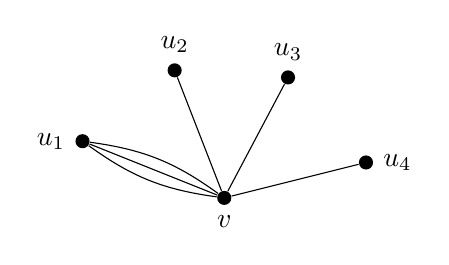
\begin{tikzpicture}[scale=.9,
  vertex/.style={circle,fill=black,inner sep=1.8pt}]
\node[vertex,label=below:$v$] (v) at (0,0) {};
\node[vertex,label=left:$u_1$] (u1) at (-2,0.8) {};
\node[vertex,label=above:$u_2$] (u2) at (-.7,1.8) {};
\node[vertex,label=above:$u_3$] (u3) at (.9,1.7) {};
\node[vertex,label=right:$u_4$] (u4) at (2,0.5) {};

\draw (v) to[bend left=14] (u1);
\draw (v) -- (u1);
\draw (v) to[bend right=14] (u1);
\draw (v) -- (u2);
\draw (v) -- (u3);
\draw (v) -- (u4);
\end{tikzpicture}
\caption{A multistar centered at $v$.  Loops, which may occur at any vertex, are not shown.}
\label{fig:multistar}
\end{figure}


\begin{proposition}[Reduction to multistars]\label{prop:4term-reduction}
  Let $H$ be a connected graph with $m$ non-loop edges.
 Then there exist a multistar $H^\ast$, graphs
$K_1,\ldots,K_N$ with $m-1$ non-loop edges, and signs $\sigma_i\in\{1,-1\}$ such that
\begin{equation}\label{eq:multistar-reduction}
 \LL_H  = \LL_{H^\ast} + t\sum_{i=1}^N\sigma_i\LL_{K_i}.
\end{equation}
Thus, the $4$-term relation, multiplicativity, and the values on multistars determine $\LL_G$ for every graph $G$.
\end{proposition}

\begin{proof}
  The basic move is the following consequence of Theorem~\ref{thm:4term}.
  Suppose in a graph $H$ a vertex $w$ is connected
to two other vertices $v$ and $u$ by edges
$b=wu$ and $c=wv$. Let $a=vu$ be a new edge.
Consider graphs $ H_0=H-\{b,c\}$ and $H'=H_0+\{a,c\}$.
  Applying~\eqref{eq:4term} to the triple $u,v,w$ gives
  \begin{equation}\label{eq:edge-slide}
    \LL_H
    =
    \LL_{H'}
    +
    t\bigl(\LL_{H_0+b}-\LL_{H_0+a}\bigr).
  \end{equation}
  We refer to the passage from $H$ to $H'$ as sliding the edge $b=wu$ across the edge $c=vw$ to the edge $a=vu$.  Notice that $H$ and $H'$ have the
  same number of non-loop edges, whereas graphs $H_0+a$ and $H_0+b$ in~\eqref{eq:edge-slide} have one fewer non-loop edge.
\medskip

Pick a vertex $v\in V(H)$.
We first move all non-loop edges onto $v$.  If some non-loop edge is not
incident to $v$, then, since $H$ is connected, there exists a path $v-w-u$
whose second edge $b=wu$ is not incident to $v$.  Let $c=vw$.  Applying the edge slide~\eqref{eq:edge-slide}
replaces $b=wu$ in $H$ by the new edge $a=vu$
decreasing the number of non-loop edges not incident to $v$ by one and adding two correction terms have $m-1$ non-loop edges.
Repeating this operation gives
\begin{equation}\label{eq:star-reduction}
   \LL_H
   =
   \LL_{H_1}
   +
   t\sum_i\sigma_i\LL_{K_i},
\end{equation}
where every non-loop edge of $H_1$ is incident to $v$ and every $K_i$ has $m-1$ non-loop edges.

It remains to concentrate all excess multiplicity at one neighbor.  Let $u$ be a vertex adjacent to $v$.
Suppose another vertex $u'\ne u$ is connected to $v$ by at least two parallel edges.
We transfer one copy of $vu'$ to $vu$ by two edge slides.

First slide one copy of $vu'$ across $uv$ replacing that copy of $vu'$ a new edge $uu'$.
Since at least one copy of $vu'$ remains, we can now
slide the new edge $uu'$ across a remaining copy of $vu'$ to a new copy of $vu$.
This decreases the multiplicity of the edge $vu'$ by one, while every correction term produced
by either slide has $m-1$ non-loop edges.
%
Repeating this two-slide operation for every $u'\ne u$ with
$\mult(vu')>1$ produces a multistar $H^\ast$ centered at $v$.
Collecting all correction terms gives~\eqref{eq:multistar-reduction}.

For a disconnected graph we apply the argument to its components.
Since every correction graph has fewer non-loop edges, the final assertion follows
by induction on their number using multiplicativity.
\end{proof}

The loopy polynomial of multistars can be evaluated explicitly using the forest expansion.

\begin{proposition}[Loopy polynomial of a multistar]
\label{prop:multistar-formula}
Let $H$ be a multistar centered at $v$
with other vertices $u_1,\ldots,u_d$ such that
$v$ is connected to $u_1$ by $r\ge 1$ edges
and to $u_i$, for $2\leq i\leq d$, by a single edge $vu_i$.
Let $\lambda_0$ be the number of loops at $v$ and $\lambda_i$ the number of loops at $u_i$.  For $S\subseteq I:=\{2,\ldots,d\}$ define
\[
   a(S):=\lambda_0+|S|+\sum_{i\in S}\lambda_i.
\]
Then
\begin{equation}\label{eq:multistar-formula}
\LL_M(t,\bx)=t^{r+d-1}\sum_{S\subseteq I}t^{-|S|}
\prod_{i\in I\setminus S}x_{\lambda_i}
\left(x_{a(S)}x_{\lambda_1}+\sum_{j=1}^r t^{-j}x_{a(S)+\lambda_1+j}\right).
\end{equation}
For a one-vertex multistar with $\lambda_0$ loops this gives $\LL_M=x_{\lambda_0}$, in agreement with~\eqref{eq:init}.
\end{proposition}

\begin{proof}
  Apply Theorem~\ref{thm:forests-sum}.
  Let $b_1<\ldots<b_r$ be the ordering of parallel edges.
  A spanning forest of $H$ contains an arbitrary subset
\[
F_S=\{vu_i : i \in S\}, \qquad   S \subseteq I,
\]
of the simple spokes, and contains either none or exactly one of the parallel edges $b_1,\ldots,b_r$.

If no $b_j$ is chosen, then $u_1$ is a singleton component.
No edge in the parallel collection is externally active, while all loops are externally active.
The resulting term is
\[
 t^{\,r+d-1-|S|}
 x_{a(S)}x_{\lambda_1}
 \prod_{i\in I\setminus S}x_{\lambda_i}.
\]

If $b_j$ is chosen, then precisely
$  b_1,\ldots,b_{j-1}$
of the parallel edges are externally active: each forms a two-edge
cycle with $b_j$ and is the least edge of that cycle.
Thus the central component contributes
  $ x_{a(S)+\lambda_1+j},$
and the power of $t$ is  $r+d-1-|S|-j.$
%
Summing these terms over $S$ and $j$ gives
\eqref{eq:multistar-formula}.
\end{proof}

\section{Examples and explicit formulas}\label{sec:examples}

We collect here the values of $\LL_G$ for a few families for which the forest expansion can
be evaluated in closed form.  We end with the smallest example showing that
$\LL_G$ contains genuinely nonmatroidal information.

\begin{proposition}[Two-vertex graphs]\label{prop:multiedge}
Let $G_m$ have two vertices joined by $m$ multiple edges.  Then
\begin{equation}\label{eq:multiedge}
 \LL_{G_m}=x_m+tx_{m-1}+\cdots+t^{m-1}x_1+t^mx_0^2 .
\end{equation}
In particular $\LL_{P_2}=x_1+tx_0^2$.  Compare with
Proposition~\ref{prop:multistar-formula}, of which this is the case of a single
leaf, and Example~\ref{ex:loop-necessary}, where the two-vertex multigraphs
occur inside a looped path.
\end{proposition}

\begin{proof}
A spanning forest is either empty or a single edge.  For $F=\varnothing$ the
two vertices are separate components, so no edge has both endpoints in one
component and $\eps(F)=0$.  The weight is $t^{m}x_0^2$.  If
$F=\{e_j\}$, where $e_j$ is the $j$-th edge in the chosen order, then for
$e\ne e_j$ the unique cycle of $F\cup\{e\}$ is $\{e_j,e\}$, so $e$ is
externally active exactly when $e<e_j$.  Hence
$\eps_F=j-1$ and the weight is $t^{m-j}x_{j}$.  Summing over
$j=1,\dots,m$ gives~\eqref{eq:multiedge}.
\end{proof}

\begin{proposition}[Paths]\label{prop:path}
For the path graph $P_m$ on $m$ vertices, put
\[
 \Lambda_m=\left\{(a_0,\ldots,a_{m-1})\in\ZZ_{\ge 0}^{m}:
 \sum_{i=0}^{m-1}(i+1)a_i=m\right\},\qquad |\ba|=\sum_i a_i.
\]
Then
\begin{equation}\label{eq:path}
 \LL_{P_m}(t,\bx)=
 \sum_{\ba\in\Lambda_m}
 \binom{|\ba|}{a_0,\ldots,a_{m-1}}
 t^{|\ba|-1}\prod_{i=0}^{m-1}x_i^{a_i}.
\end{equation}
\end{proposition}

\begin{proof}
Every subset of $E(P_m)$ is a spanning forest, and no nonforest edge lies on
a cycle, so $\eps(F)=0$ for all $F$.  Deleting $m-1-|F|$ of the $m-1$
edges leaves $m-|F|$ components whose orders form a composition of $m$ into
$m-|F|$ parts. Writing $a_i$ for the number of components with $i+1$ vertices
gives $|\ba|=m-|F|$ and $\sum_i(i+1)a_i=m$.  The number of compositions with
these part multiplicities is the multinomial coefficient
$\ds \binom{|\ba|}{a_0,\ldots,a_{m-1}}$, and the weight of each such forest is
$t^{(m-1)-|F|}\prod_i x_i^{a_i}=t^{|\ba|-1}\prod_i x_i^{a_i}$.
\end{proof}

For example,
  \begin{equation}
    \label{eq:path4}
 \LL_{P_3}=x_2+2tx_0x_1+t^2x_0^3,
 \qquad
 \LL_{P_4}=x_3+2t x_0x_2+t x_1^2+3t^2x_0^2x_1+t^3x_0^4.
\end{equation}

The next family is the smallest one in which external activity contributes (it is also the case $\eps(F)\le1$ of the unicyclic analysis of
Section~\ref{subsec:unicyclic}).

\begin{proposition}[Cycles]\label{prop:cycle}
For the simple cycle $C_m$, $m\ge 3$, let
\[
 \Lambda'_m = \left\{(a_0,\ldots,a_{m-2})\in\ZZ_{\ge 0}^{m-1}:
 \sum_{i=0}^{m-2}(i+1)a_i=m,\quad |\ba|\ge 2\right\}
\qquad \text{and} \qquad
 \gamma_{\ba}=\frac{m}{|\ba|}
 \binom{|\ba|}{a_0,\ldots,a_{m-2}}.
\]
Then
\begin{equation}\label{eq:circle}
 \LL_{C_m}=x_m+(m-1)tx_{m-1}
 +\sum_{\ba\in\Lambda'_m}\gamma_{\ba}t^{|\ba|}
 \prod_{i=0}^{m-2}x_i^{a_i}.
\end{equation}
\end{proposition}

\begin{proof}
The spanning forests of $C_m$ are the proper subsets of $E(C_m)$.  If
$|F|=m-1$, the single nonforest edge $e$ closes the whole cycle, so it is
externally active precisely when it is the least edge.  This gives $x_m$ for
that one forest and $tx_{m-1}$ for each of the remaining $m-1$.  If
$|F|\le m-2$, then at least two edges are missing, every nonforest edge joins
two distinct components, and $\eps(F)=0$.  The components are the arcs
cut out by the $p:=m-|F|$ missing edges, so their orders form a \emph{cyclic}
composition of $m$ into $p$ parts, of which there are
$\ds \frac mp \binom{p}{a_0,\ldots,a_{m-2}} = \gamma_{\ba}$, each contributes
$t^{m-|F|}\prod_i x_i^{a_i}=t^{|\ba|}\prod_i x_i^{a_i}$.
\end{proof}

In particular,
\[ \LL_{C_3}=x_3+2tx_2+3t^2x_0x_1+t^3x_0^3,
 \qquad
 \LL_{C_4}=x_4+3tx_3+2t^2x_1^2+4t^2x_0x_2
 +4t^3x_0^2x_1+t^4x_0^4.
\]

\begin{proposition}[Stars with loops]\label{prop:star}
Let $S_{m,\ell}$ be a star with $m$ edges and $\ell$ loops at its center.
Then
\begin{equation}\label{eq:star}
\ds \LL_{S_{m,\ell}}=
 \sum_{i=0}^{m}\binom mi(tx_0)^i x_{\ell+m-i},
\end{equation}
and in particular $\ds \LL_{S_m}=\sum_{i=0}^{m}\binom mi(tx_0)^i x_{m-i}$.
The case $\ell=0$, $m=3$ is used in Remark~\ref{rem:nonmatroidal-example}.
\end{proposition}

\begin{proof}
A spanning forest is a subset $F$ of the $m$ star edges.  It has one component
containing the center, with $1+|F|$ vertices, and $m-|F|$ isolated leaves.
Each of the $\ell$ loops is a one-edge cycle and is therefore externally
active and is assigned to the center component. A nonforest star edge joins
two distinct components and is not active.  Hence
$\eps_F(\text{center})=\ell$ and the weight is
$t^{(m+\ell)-|F|-\ell}x_{|F|+\ell}x_0^{m-|F|}$.  Setting $i=m-|F|$ and summing
over the $\binom mi$ choices gives~\eqref{eq:star}.
\end{proof}

Alternatively, \eqref{eq:star} can be obtained as the specialization of the
general multistar formula~\eqref{eq:multistar-formula} with $r=1$, $d=m$,
$\lambda_0=\ell$, and $\lambda_i=0$ for every leaf.

\begin{remark}[A nonmatroidal  comparison]\label{rem:nonmatroidal-example}
The path and star formulas give a simple illustration of the genuinely
nonmatroidal information contained in the loopy polynomial.  The two four-vertex trees,
the path $P_4$ and the star $S_{3,0}=K_{1,3}$ have the same Tutte polynomial,
whereas from~\eqref{eq:path4} and~\eqref{eq:star} we have
\[
  \LL_{P_4}=x_3+2t x_0x_2+t x_1^2+3t^2x_0^2x_1+t^3x_0^4 \quad \text{and} \quad \LL_{K_{1,3}}
 =x_3+3t x_0x_2
  +3t^2x_0^2x_1+t^3x_0^4.
\]
Thus $\LL$ distinguishes these two graphs.  This example also reflects the
degree-sequence result of Theorem~\ref{thm:L-degree-sequence}: the two degree
generating polynomials are
\[
 \sum_{v\in V(P_4)} t^{d(v)}=2t+2t^2,
 \qquad
 \sum_{v\in V(K_{1,3})} t^{d(v)}=3t+t^3.
\]
\end{remark}


\section{Vertex deletion and subgraph profiles}\label{sec:vertex-deletion}

The forest expansion singles out the behavior of one of the variables of $\LL_G$.  For a loopless graph the variable $x_0$ marks isolated vertices, so
differentiating with respect to it amounts to deleting a vertex, and iterating gives access to statistics of induced subgraphs.

\subsection{The vertex-deletion identity}\label{subsec:degree-sequence}

For a loopless graph, the variable $x_0$ has a particularly simple meaning in
the forest expansion: a component contributes $x_0$ if and only if it is an
isolated vertex.  Marking such a component
leads to a \emph{vertex-deletion identity}.

\begin{proposition}[Vertex-deletion identity]\label{prop:vertex-deletion}
Let $G$ be a loopless graph.  Then
\begin{equation}\label{eq:vertex-deletion}
   \frac{\partial}{\partial x_0}\LL_G(t,\bx)
   =
   \sum_{v\in V(G)}
   t^{d(v)}\LL_{G-v}(t,\bx),
\end{equation}
where $d(v)$ counts multiple edges with multiplicity.
\end{proposition}

\begin{proof}
  Differentiate the forest expansion~\eqref{eq:forests}.
Since $G$ is loopless, a component of a spanning forest contributes $x_0$ precisely when
it consists of a single isolated vertex $v$.  After marking this singleton
component and deleting it, what remains is an arbitrary spanning forest $F'$ of $G-v$.

No edge incident with $v$ is externally active with respect to
$\{v\}\sqcup F'$, since its endpoints lie in different components.
The external activity of every remaining edge is exactly its external activity
in $G-v$.  Passing from $G$ to $G-v$ removes precisely $d(v)$ edges, and therefore
\[
   \wt_G(\{v\}\sqcup F')
   =
   x_0\,t^{d(v)}\wt_{G-v}(F').
\]
Summing over $v$ and $F'$ gives~\eqref{eq:vertex-deletion}.
If a forest has several isolated vertices, it occurs once for each choice of the marked
singleton, exactly as required by differentiation.
\end{proof}

The identity becomes especially useful after one simple specialization.

\begin{lemma}\label{lem:constant-specialization}
For every graph $G$ with $n$ vertices,
\begin{equation}\label{eq:constant-specialization}
   \left.
      \LL_G(t,\bx)
   \right|_{x_0=x_1=\cdots=(1-t)^{-1}}
   =(1-t)^{-n}.
\end{equation}
\end{lemma}

\begin{proof}
Work over $\QQ(t)$ and substitute $c=(1-t)^{-1}$.  If $G$ has no non-loop
edges, multiplicativity and the defining initial condition give $c^n$.  If $e$ is a non-loop edge, induction and loopy deletion-contraction give
\[
   c^{n-1}+t c^n
   =c^n\bigl((1-t)+t\bigr)
   =c^n.
\]
\end{proof}
\subsection{The degree sequence}\label{subsec:degree-sequence-thm}


\begin{theorem}\label{thm:L-degree-sequence}
The loopy polynomial determines the degree sequence of every loopless graph.  More precisely, if $G$ has $n$ vertices, then
\begin{equation}\label{eq:degree-generating-function}
   \sum_{v\in V(G)}t^{d(v)}
   =
   (1-t)^{n-1}
   \left.
      \frac{\partial}{\partial x_0}\LL_G(t,\bx)
   \right|_{x_0=x_1=\cdots=(1-t)^{-1}}.
\end{equation}
\end{theorem}

\begin{proof}
Apply Lemma~\ref{lem:constant-specialization} to every term on the right-hand
side of~\eqref{eq:vertex-deletion}.  Since each $G-v$ has $n-1$ vertices,
\[
   \left.
      \frac{\partial}{\partial x_0}\LL_G(t,\bx)
   \right|_{x_i=(1-t)^{-1}}
   =
   (1-t)^{-(n-1)}
   \sum_{v\in V(G)}t^{d(v)},
\]
giving~\eqref{eq:degree-generating-function}.  The coefficient of $t^d$ in this polynomial
is the number of vertices of degree $d$.
\end{proof}


Theorem~\ref{thm:L-degree-sequence} illustrates a useful feature of the loopy polynomial that is already visible in its forest expansion.
For a loopless graph, $x_0$ marks singleton forest components and no other components.
Differentiation with respect to $x_0$ therefore singles out a vertex, while the power of $t$ records the number of edges incident to it.
The degree generating function is obtained by summing over the remaining forest data through the constant specialization of Lemma~\ref{lem:constant-specialization}.

The loopless hypothesis is essential for this argument.
If a vertex carries loops, its singleton forest component contributes a variable $x_r$
with $r>0$, and the same variable can also arise from a nonsingleton component.
Thus no single variable uniformly marks vertices.
Multiple edges, by contrast, cause no difficulty in the argument.
A refined version of the loopy polynomial will later remove this ambiguity,
see Theorem~\ref{thm:degree-sequence-loops}.


Proposition~\ref{prop:vertex-deletion} is the first case of the higher vertex-deletion identity below.
Marking several singleton components at once recovers considerably more than the degree sequence,
including the complete induced edge count profile.

\subsection{Higher vertex deletion}\label{subsec:induced-edge-profile}

The preceding degree-sequence result is the first case of a hierarchy of
vertex-deletion identities.  Higher derivatives with respect to $x_0$ mark
several singleton components simultaneously and recover considerably more
information than the degree sequence.

Recall that for $S\subseteq V(G)$, $\kp_G(S)$ is the number of edges of $G$
having at least one endpoint in $S$, each edge counted once, equivalently
$\kp_G(S)=m(G)-m(G-S)$.

\begin{proposition}[Higher vertex-deletion identity]
\label{prop:higher-vertex-deletion}
Let $G$ be a loopless graph on $n$ vertices.  For $0\le k\le n$,
\begin{equation}\label{eq:higher-vertex-deletion}
   \frac{\partial^k}{\partial x_0^k}\LL_G(t,\bx)
   =
   k!\sum_{\substack{S\subseteq V(G)\\ |S|=k}}
      t^{\kp_G(S)}\LL_{G-S}(t,\bx).
\end{equation}
\end{proposition}

\begin{proof}
Differentiate the forest expansion~\eqref{eq:forests}.  Since $G$ is
loopless, a component of a spanning forest contributes $x_0$ if and only if
it is a singleton vertex.  Thus a term contributing to the $k$th derivative
amounts to a spanning forest together with a choice of $k$ singleton
components.

Fix a set $S\subseteq V(G)$ of $k$ such vertices.  Removing the singleton
components indexed by $S$ gives an arbitrary spanning forest $F'$ of $G-S$.
Conversely, every spanning forest $F'$ of $G-S$ gives the spanning forest $F=F'\sqcup\{\{v\}:v\in S\}$  of $G$.

No edge incident with $S$ is externally active with respect to $F$, since such an edge has its endpoints in distinct components of $F$.
Every edge whose endpoints lie in $V(G)\setminus S$ has exactly the same external activity status
with respect to $F$ as it has with respect to $F'$ in $G-S$. Therefore   $\eps_G(F)=\eps_{G-S}(F'),$
and the componentwise activities of all components inherited from $F'$ are unchanged.  Moreover,
\[
 m(G)-m(G-S)=\kp_G(S)    \quad \text{and} \quad    |F|=|F'|.
\]
The corresponding weights satisfy
\[
   \wt_G(F)
   =
   x_0^k\,t^{\kp_G(S)}\wt_{G-S}(F').
\]
If $F$ has $a$ singleton components, then
\[
   \frac{\partial^k}{\partial x_0^k}x_0^a
   =k!\binom ak x_0^{a-k}.
\]
On the right-hand side of~\eqref{eq:higher-vertex-deletion}, the same forest
is counted once for each of the $\binom ak$ admissible choices of $S$.
This proves the identity.
\end{proof}

\begin{remark}[The bridge to the polyhedral half]\label{rem:kappa-bridge}
The exponent $\kp_G(S)$ in~\eqref{eq:higher-vertex-deletion} is exactly the
submodular rank function whose polymatroid carries the bizonotopal geometry of
Section~\ref{sec:polyhedral}.  The same edge-incidence statistic therefore
appears twice in this paper, and for different reasons: here it is forced on us
by iterated vertex deletion on the loopy side, and in
Section~\ref{sec:polyhedral} it is the rank function
$\ba(S)\le\kp_G(S)$ defining the score polytope $P_G$.  This is the first
point of contact between the combinatorial and the polyhedral halves of the
paper.  The second is Corollary~\ref{cor:polytope-specialization}, where the
component weight $|E(T)|+\eps_F(T)$ of the forest
expansion~\eqref{eq:forests} turns out to be the length of an interval factor
in a polyhedral decomposition of $P_G$.
\end{remark}

Combining Proposition~\ref{prop:higher-vertex-deletion} with the constant
specialization of Lemma~\ref{lem:constant-specialization} gives a generating
function for the values of $\kp_G$ on subsets of fixed cardinality.

\subsection{Induced-edge and \texorpdfstring{$\kp$}{kappa}-profiles}\label{subsec:induced-profiles}

\begin{corollary}\label{cor:kappa-profile}
Let $G$ be a loopless graph on $n$ vertices.  Then, for $0\le k\le n$,
\begin{equation}\label{eq:kappa-profile}
   \sum_{\substack{S\subseteq V(G)\\ |S|=k}}
      t^{\kp_G(S)}
   =
   \frac{(1-t)^{n-k}}{k!}
   \left.
      \frac{\partial^k}{\partial x_0^k}\LL_G(t,\bx)
   \right|_{x_0=x_1=\cdots=(1-t)^{-1}} .
\end{equation}
\end{corollary}

\begin{proof}
  Every graph $G-S$ occurring in~\eqref{eq:higher-vertex-deletion} has $n-k$ vertices,
so Lemma~\ref{lem:constant-specialization} gives
\[
   \left.
      \LL_{G-S}(t,\bx)
   \right|_{x_i=(1-t)^{-1}}
   =(1-t)^{-(n-k)}.
\]
Substitution in~\eqref{eq:higher-vertex-deletion} gives
\eqref{eq:kappa-profile}.
\end{proof}

The crucial point is that the specialization in Lemma~\ref{lem:constant-specialization} is uniform in $S$: every
$\LL_{G-S}$ with $|S|=k$ becomes the same value $(1-t)^{-(n-k)}$.  Thus one never has to disentangle the individual
polynomials $\LL_{G-S}$ occurring in the weighted sum
\eqref{eq:higher-vertex-deletion}. After specialization the sum simply collapses to the left-hand side of~\eqref{eq:kappa-profile}.

Recall that $e_G(S)$ denotes the number of edges of the induced subgraph
$G[S]$, counted with multiplicity.  For $0\le s\le n$ and $j\ge 0$ put
\begin{equation}\label{eq:induced-edge-array}
   N_G(s,j)
   :=
   \#\{S\subseteq V(G): |S|=s,\ e_G(S)=j\}.
\end{equation}
We call the numerical array $\bigl(N_G(s,j)\bigr)_{s,j}$ the
\emph{induced edge count profile} of $G$.  Equivalently, for each $s$ it is
encoded by the polynomial
\begin{equation}\label{eq:induced-edge-polynomial}
   \cE_{G,s}(q)
   :=
   \sum_{\substack{S\subseteq V(G)\\ |S|=s}}q^{e_G(S)}
   =\sum_{j\ge 0}N_G(s,j)q^j.
\end{equation}

\begin{theorem}\label{thm:induced-edge-profile}
The loopy polynomial of a loopless graph determines its
induced edge count profile.  More explicitly, define
\begin{equation}\label{eq:Delta-definition}
   \Delta_{G,k}(t)
   :=
   \frac{(1-t)^{n-k}}{k!}
   \left.
      \frac{\partial^k}{\partial x_0^k}\LL_G(t,\bx)
   \right|_{x_0=x_1=\cdots=(1-t)^{-1}} .
\end{equation}
Then
\begin{equation}\label{eq:induced-edge-from-L}
   \cE_{G,s}(q)
   =
   q^{m(G)}\Delta_{G,n-s}(q^{-1}),
   \qquad 0\le s\le n.
\end{equation}
\end{theorem}

\begin{proof}
By Corollary~\ref{cor:kappa-profile},
\[
   \Delta_{G,n-s}(t)
   =
   \sum_{\substack{R\subseteq V(G)\\ |R|=n-s}}
      t^{\kp_G(R)}.
\]
Put $S=V(G)\setminus R$.  Then $|S|=s$, and an edge is not incident with
$R$ precisely when both of its endpoints lie in $S$.  Hence
\[
   \kp_G(R)=m(G)-e_G(S).
\]
Therefore
\[
   \Delta_{G,n-s}(t)
   =
   \sum_{|S|=s}t^{m(G)-e_G(S)}.
\]
Replacing $t$ by $q^{-1}$ and multiplying by $q^{m(G)}$ gives
\eqref{eq:induced-edge-from-L}.
\end{proof}

Several familiar graph invariants are immediate consequences.

\begin{corollary}\label{cor:independence-clique}
Let $G$ be a loopless graph.
\begin{enumerate}[(1)]
\item The loopy polynomial determines the independence polynomial
  \begin{equation}
    \label{eq:independence}
   I_G(z)=\sum_{s=0}^{n} i_s(G)z^s,
 \end{equation}
where $i_s(G)$ is the number of independent sets of cardinality $s$.  Indeed,
\begin{equation}\label{eq:independence-from-edge-profile}
   i_s(G)=[q^0]\cE_{G,s}(q).
\end{equation}

\item If $G$ is simple, then $\LL_G$ determines the clique polynomial.  The
number $c_s(G)$ of $s$-vertex cliques is
\begin{equation}\label{eq:cliques-from-edge-profile}
   c_s(G)
   =[q^{\binom{s}{2}}]\cE_{G,s}(q).
\end{equation}

\item If $G$ is simple, then $\LL_G$ determines the induced edge count
profile of the complement.  More precisely,
\begin{equation}\label{eq:complement-edge-profile}
   \cE_{\overline G,s}(q)
   =
   q^{\binom{s}{2}}\cE_{G,s}(q^{-1}).
\end{equation}
\end{enumerate}
\end{corollary}

\begin{proof}
A set $S$ is independent precisely when $e_G(S)=0$, which proves~(1).
For a simple graph, an $s$-vertex set induces $\binom{s}{2}$ edges precisely
when it is a clique, proving~(2).  Finally, (3) follows, since
$   e_{\overline G}(S)=\binom{s}{2}-e_G(S) $
for every $s$-vertex set $S$.
\end{proof}

Part~(3) gives a partial answer to Problem~\ref{prob:complement}: the loopy polynomial
determines the complete induced edge count profile of the
complement, even though it is not known whether it determines $\LL_{\overline G}$ itself.

It is useful to compare these conclusions with the corresponding information
in the $U$-polynomial, the polychromate, and the Tutte symmetric
function.  The independence polynomial $I_G$~\eqref{eq:independence} is already known to be determined by
$U_G$.  Noble and Welsh~\cite[Theorem~5.2]{NW} (see also~\cite[Theorem~26.37]{Nob}) proved that the stability polynomial
\[
  A_G(p)  =
  \sum_{\substack{S\subseteq V(G)\\S\text{ independent}}}
  p^{|S|}(1-p)^{n-|S|} =(1-p)^n I_G\!\left(\frac{p}{1-p}\right),
\]
the probabilistic normalization of $I_G$, is the specialization
\[
  A_G(p)  =
  \left.
    U_G(\bz,y)\right|_{y=0,\ z_1=1,\ z_j=-(-p)^j\ (j\ge 2)}.
  \]

Combining this with the fact that every monomial of
$U_G$ has weighted $z$-degree $n$, we obtain the direct specialization
\begin{equation}\label{eq:independence-from-U}
 I_G(z) = \left.   U_G(\bz,y) \right|_{y=0,\ z_1=1+z,\ z_j=(-1)^{j+1}z^j\ (j\ge 2)}.
\end{equation}
For simple graphs the clique numbers are likewise directly visible in
$U_G$, see~\cite[Proposition~26.38]{Nob}.

The comparison with the polychromate is sharper.  For $2\le s\le n$,
\begin{equation}\label{eq:edge-profile-from-polychromate}
   [q_s q_1^{\,n-s}]\,\eta_G(\bq,y)
   =
   \cE_{G,s}(y).
\end{equation}
Indeed, a partition of type $(s,1^{n-s})$ with $s\ge 2$ is uniquely determined
by its $s$-element block, and, because $G$ is loopless, its internal edges are
exactly the edges induced by that block.  Thus Theorem~\ref{thm:induced-edge-profile}
shows that $\LL_G$ directly recovers the entire family of polychromate
coefficients of partition type $(s,1^{n-s})$, not merely the coefficient of
type $(n-1,1)$ used above to recover the degree sequence.  By the equivalence
$\eta_G\longleftrightarrow U_G$ of Sarmiento~\cite{Sar} (and its extension in
Merino--Noble~\cite{MN}), this also gives another route from $U_G$ to the
full induced edge count profile.

The range in~\eqref{eq:edge-profile-from-polychromate} is genuinely
$2\le s\le n$.  At $s=1$ the indicated monomial becomes $q_1^n$, whose
coefficient in $\eta_G$ is $1$, rather than $\cE_{G,1}(y)=n$.
The entry $s=0$ is also not represented by such a partition monomial.
Of course these two profile entries are already fixed by
$n$, namely $\cE_{G,0}(y)=1$ and $\cE_{G,1}(y)=n$.

By contrast, the analogous formula for Stanley's Tutte symmetric function
does hold already at $s=1$.  In the normalization of
\eqref{eq:XB-coloring},
\begin{equation}\label{eq:edge-profile-from-XB}
   \cE_{G,s}(y)
   =
   \frac{1}{(n-s)!}
   [m_{(s,1^{n-s})}]\,\XB_G(y-1;\bw),
   \qquad 1\le s\le n.
\end{equation}
For $s\ge 2$, the repeated color singles out the $s$-vertex color class, the remaining colors may be assigned in $(n-s)!$ ways,
and the monochromatic edges are precisely the edges induced by that class.
At $s=1$ one checks the formula separately:
\[
   [m_{(1^n)}]\XB_G=n!,
   \qquad
   \frac{n!}{(n-1)!}=n=\cE_{G,1}(y).
\]
At $y=0$, formula~\eqref{eq:edge-profile-from-XB} reduces to the familiar
recovery of independent sets from $X_G=\XB_G(-1;\bw)$.

Thus the full part of partition type $(s,1^{n-s})$ that is transparent for
$\eta_G$ and $\XB_G$ is recovered from $\LL_G$ by higher vertex deletion.



\section{Relations with other graph polynomials}\label{sec:relations}

The spanning-forest expansion of  Theorem~\ref{thm:forests-sum} places the
loopy polynomial in a classical circle of ideas going back to Tutte's 1947 paper~\cite{Tu1}.
In this section we make the connection precise, comparing $\LL_G$ in turn with Tutte's universal $V$-function, the $U$-polynomial
of Noble and Welsh, and Brylawski's polychromate.  What the comparisons have in common is that each of these invariants is a different compression of
the same componentwise statistic $\bigl(|V(T)|,\eps_F(T)\bigr)$.  The object
that keeps both coordinates is the refined loopy polynomial of Section~\ref{sec:refined}.

\subsection{Tutte's universal \texorpdfstring{$V$}{V}-function}\label{subsec:universal-V}

We first recall the form of Tutte's universal $V$-function that is most
convenient for comparison with the loopy polynomial.
Let $L_r$ denote, as before, the graph consisting of one vertex
with $r$ loops.  A $V$-function with values in a commutative ring $R$ is a multiplicative graph invariant
$V$ satisfying
\begin{equation}\label{eq:V-deletion-contraction}
   V_G=V_{G-e}+V_{G_e}
\end{equation}
for every non-loop edge $e$, where $G_e$ denotes ordinary contraction.
Tutte proved that the values of such a function on the graphs $L_r$ may be
prescribed arbitrarily and determine the function uniquely~\cite{Tu1}.
Equivalently, there is a universal polynomial
  $ \cV_G(\bv)=\cV_G(v_0,v_1,\ldots)$
characterized by~\eqref{eq:V-deletion-contraction}, multiplicativity, and the initial conditions
  $\cV_{L_r}(\bv)=v_r.$

Bollob\'as, Pebody and Riordan~\cite{BPR} later strengthened this universality
statement: for connected graphs it is enough to impose
deletion-contraction only on edges that are neither bridges nor loops.  The
resulting invariant still factors through Tutte's universal $V$-function.

Tutte expressed the universal $V$-function as a sum over spanning
subgraphs.  It will be useful to distinguish this set of coordinates from the
terminal-value coordinates $v_r$.  Put
\begin{equation}\label{eq:Tutte-Z}
   Z_G(\bz)
   :=
   \sum_{A\subseteq E(G)}
   \prod_{D\in c(A)} z_{\nu(D)},
   \qquad
   \nu(D):=|E(D)|-|V(D)|+1.
\end{equation}
Thus each component of a spanning subgraph contributes a variable indexed by
its cyclomatic number.

The relation between the two coordinate systems is a binomial transform.
Indeed,
\begin{equation}\label{eq:V-Z-binomial}
   Z_G(\bz)
   =
   \left.
      \cV_G(\bv)
   \right|_{
      v_r=\sum_{j=0}^r\binom{r}{j}z_j
   },
\end{equation}
and hence, by binomial inversion,
\begin{equation}\label{eq:Z-V-binomial}
   \cV_G(\bv)
   =
   \left.
      Z_G(\bz)
   \right|_{
      z_r=\sum_{j=0}^r(-1)^{r-j}\binom{r}{j}v_j
   }.
\end{equation}
This change of coordinates already appears in Tutte's construction of the universal graph ring in~\cite{Tu1}.

The activity form of the universal $V$-function was made explicit by Wang
and Sachs~\cite{WS}.  An equivalent expansion was later obtained by
Bollob\'as, Pebody and Riordan~\cite{BPR}.

\begin{theorem}[Wang--Sachs~\cite{WS}, Bollob\'as--Pebody--Riordan~\cite{BPR}]
\label{thm:V-forest}
For every ordering of $E(G)$,
\begin{equation}\label{eq:V-forest}
   \cV_G(\bv)
   =
   \sum_{F\in\cF(G)}
   \prod_{T\in c(F)}v_{\eps_F(T)}.
\end{equation}
In particular, the right-hand side is independent of the edge order.
\end{theorem}

Theorem~\ref{thm:V-forest} is the classical precursor of
Theorem~\ref{thm:forests-sum}.  It already distributes external
activity among the individual components of an arbitrary spanning forest,
rather than recording only the total activity of a maximal spanning forest.
The loopy polynomial arises from the same expansion after a simple graph
operation that inserts the missing component-size information.

\subsection{The loopy polynomial as a shifted \texorpdfstring{$V$}{V}-function}\label{subsec:loopy-V}

For a graph $G$, let $G^\circ$ be obtained by adding a new loop at every
vertex of $G$.  We call these the \emph{baseline loops}.  The following
identity gives a direct relation between the loopy polynomial and Tutte's
universal $V$-function.

\begin{proposition}\label{prop:loopy-V}
Let $m=|E(G)|$.  Then
\begin{equation}\label{eq:loopy-V-t1}
   \LL_G(1,\bx)
   =
   \left.
      \cV_{G^\circ}(\bv)
   \right|_{v_r=x_{r-1}\ (r\ge 1)}.
\end{equation}
More generally,
\begin{equation}\label{eq:loopy-V}
   \LL_G(t,\bx)
   =
   t^m
   \left.
      \cV_{G^\circ}(\bv)
   \right|_{v_r=t^{1-r}x_{r-1}\ (r\ge 1)}.
\end{equation}
\end{proposition}

\begin{proof}
The spanning forests of $G^\circ$ are exactly the spanning forests of $G$.
Every loop is externally active, and the baseline loop at a vertex of
a component $T$ is assigned to $T$.  Hence the number of externally active
edges assigned to $T$, when the forest is regarded as a forest of $G^\circ$, is
\[
   |V(T)|+\eps_F(T).
\]
Applying Theorem~\ref{thm:V-forest} therefore gives
\[
   \cV_{G^\circ}(\bv)
   =
   \sum_{F\in\cF(G)}
   \prod_{T\in c(F)}
   v_{|V(T)|+\eps_F(T)}.
\]
The substitution $v_r=x_{r-1}$ gives~\eqref{eq:loopy-V-t1}.
For the second identity, substitute instead
$v_r=t^{1-r}x_{r-1}$.  The resulting power of
$t$, before multiplication by $t^m$, is
\[
   \sum_{T\in c(F)}
      \bigl(1-|V(T)|-\eps_F(T)\bigr)
   =|c(F)|-|V(G)|-\eps(F)
   =-|F|-\eps(F).
\]
Thus~\eqref{eq:loopy-V} is exactly the forest expansion
\eqref{eq:forests}.
\end{proof}

There is also a recursive way to see~\eqref{eq:loopy-V-t1}.  If $e=uv$ is
a non-loop edge of $G$, ordinary contraction of $e$ in $G^\circ$ leaves the
two baseline loops at $u$ and $v$ as two loops at the contracted vertex.  On
the other hand, loopy contraction of $e$ in $G$ leaves $e$ itself as a loop,
and passing to $(G/e)^\circ$ adds one baseline loop at the new vertex.  Thus
\[
   G^\circ_e\cong (G/e)^\circ.
\]
In this sense the baseline loops convert ordinary contraction into loopy contraction.

Proposition~\ref{prop:loopy-V} identifies the ungraded loopy polynomial with a classical invariant evaluated on a simple modification of the graph.

What is special about the loopy polynomial is therefore not the existence
of a deletion-contraction invariant, but the particular way in which component size and activity are combined.
In Section~\ref{sec:refined} we return to this point and introduce a refinement that keeps these two
quantities separate.

\subsection{The  \texorpdfstring{$U$}{U}-polynomial}
\label{subsec:ordinary-U-polychromate}

The ordinary $U$-polynomial of Noble and Welsh~\cite{NW,Nob} is
\begin{equation}\label{eq:ordinary-U}
   U_G(\bz,y)
   =
   \sum_{A\subseteq E(G)}
   \left(\prod_{D\in c(A)}z_{|V(D)|}\right)
   (y-1)^{\sum_{D\in c(A)}\nu(D)}.
\end{equation}
The activity intervals of Lemma~\ref{lem:activity-intervals} put it into
spanning-forest form.

\begin{proposition}\label{prop:U-forest}
For every graph $G$,
\begin{equation}\label{eq:U-forest}
   U_G(\bz,y)
   =
   \sum_{F\in\cF(G)}
   y^{\eps(F)}
   \prod_{T\in c(F)}z_{|V(T)|}.
\end{equation}
\end{proposition}

\begin{proof}
Fix an edge order and apply Lemma~\ref{lem:activity-intervals}, which writes
$2^{E(G)}$ as the disjoint union of the intervals
$[F,F\cup\EA(F)]$ over spanning forests $F$.  Let
$A=F\cup J$ with $J\subseteq\EA(F)$.  Every edge of $J$ has both
endpoints in a single component of $F$, so $(V(G),A)$ and $F$ have the same
components. In particular
\[
  \prod_{D\in c(A)}z_{|V(D)|}=\prod_{T\in c(F)}z_{|V(T)|} \qquad \text{and} \qquad  \sum_{D\in c(A)}\nu(D)=|A|-|F|=|J| .
\]
Summing~\eqref{eq:ordinary-U} over the interval therefore gives
\[
   \Bigl(\prod_{T\in c(F)}z_{|V(T)|}\Bigr)
   \sum_{J\subseteq\EA(F)}(y-1)^{|J|}
   =
   y^{\eps(F)}\prod_{T\in c(F)}z_{|V(T)|},
\]
since $\eps(F)=|\EA(F)|$.  Summing over $F$
gives~\eqref{eq:U-forest}.
\end{proof}

Formula~\eqref{eq:U-forest} is the spanning-forest activity expansion of Noble and Welsh~\cite{NW},
written with our activity convention, see also~\cite{Nob}.
Compared with the forest expansion~\eqref{eq:forests} of $\LL_G$, it shows how differently the two invariants record activity.
We return to this in Section~\ref{subsec:refined-extended}, where both appear as specializations of a single object.


\subsection{The polychromate}\label{subsec:polychromate}

There is another classical incarnation of the $U$-polynomial that is important for this comparison.
Brylawski introduced the \emph{polychromate} in his intersection theory for graphs~\cite{Bry}.  We write it as
\begin{equation}\label{eq:polychromate}
   \eta_G(\bq,y)
   :=
   \sum_{\pi\vdash V(G)}
   y^{e_G(\pi)}
   \prod_{B\in\pi}q_{|B|},
\end{equation}
where the sum is over all set partitions of $V(G)$ and $e_G(\pi)$ is the
number of edges of $G$ whose two endpoints lie in the same block of $\pi$.
Edges are counted with multiplicity, and a loop is internal to every block
containing its vertex.  Thus, unlike~\eqref{eq:ordinary-U}, which is organized
by spanning subgraphs and their connected components, the polychromate is
organized by partitions of the vertex set and records the sizes of their
blocks together with the number of edges internal to the blocks.

Sarmiento~\cite{Sar} proved that the polychromate and the $U$-polynomial determine one another.
Her paper is stated for simple graphs.  Merino and Noble~\cite{MN}
subsequently recovered the equivalence in a framework that
allows loops and multiple edges, see also~\cite{Nob}.  The equivalence is quite nontrivial: the
change of coordinates is triangular with respect to refinement of set
partitions, and the coefficients count coarsenings of a fixed partition type.
In the Merino--Noble formulation it may also be understood as a change
between two natural bases of the corresponding Tutte symmetric function.

Both sides of this equivalence admit natural refinements in which the
component or block data are retained separately.  These refinements will
be discussed in Section~\ref{sec:refined}.  In particular, the extended
polychromate of Bollob\'as and Riordan~\cite{BR}, called the strong
polychromate in their terminology, will provide the partition-side
description of the refined loopy polynomial, see
Section~\ref{subsec:block-statistics}.

The two ordinary descriptions are complementary: the $U$-side is adapted
to spanning subgraphs, whereas the polychromate is adapted to vertex
partitions.  Some graph-theoretic information that is not at all
transparent in the spanning-subgraph expression for $U$ becomes immediate
on the polychromate side.


A basic example is the degree sequence.  If $G$ is loopless and $n\ge 3$,
the partitions $\{\{v\},V(G)\setminus\{v\}\}$ contribute
$y^{m-d(v)}q_1q_{n-1}$, so the corresponding polychromate coefficient
recovers the degree multiplicities.  The cases $n\le2$ are immediate.
Hence $\eta_G$, and therefore $U_G$, determines the degree sequence, see
also~\cite[Proposition~26.56]{Nob}.  On the loopy side the same information came out of the vertex-deletion
identity of Section~\ref{sec:vertex-deletion}, by an entirely different
route.  The agreement of two such different mechanisms is one reason for
expecting the two invariants to be closely related.

\subsection{Chromatic symmetric functions, forests, and matchings}\label{subsec:X-and-matchings}

We finish with several useful consequences of the forest expansion that are
most naturally stated directly in terms of the loopy polynomial.

Let $X_G$ denote Stanley's chromatic symmetric function~\cite{Sta}, with the convention that $X_G=0$ when $G$ has a loop.
Its power-sum expansion is
\begin{equation}\label{eq:X-powersum}
   X_G
   =
   \sum_{A\subseteq E(G)}
   (-1)^{|A|}
   \prod_{D\in c(A)}p_{|V(D)|}.
\end{equation}
The activity intervals of Lemma~\ref{lem:activity-intervals} immediately give
an external activity version of this formula:
\begin{equation}\label{eq:X-zero-activity}
   X_G
   =
   \sum_{\substack{F\in\cF(G)\\ \eps(F)=0}}
   (-1)^{|F|}
   \prod_{T\in c(F)}p_{|V(T)|}.
\end{equation}
Indeed, the contributions from the interval of $F$ are multiplied by
$\ds \sum_{J\subseteq\EA(F)}(-1)^{|J|}$,
which vanishes unless $\EA(F)=\varnothing$.

The zero-activity part can be recognized inside the ordinary loopy polynomial.
A forest $F$ contributing a monomial
$\ds M=\prod_{i\ge 0}x_i^{a_i}$ to~\eqref{eq:forests} satisfies
\begin{equation}\label{eq:activity-from-monomial}
   \eps(F)=w(M)+\ell(M)-|V(G)|, \qquad \text{where} \quad
   \ell(M)=\sum_i a_i,
   \quad  \text{and} \quad
   w(M)=\sum_i i a_i.
\end{equation}
Thus total external activity of $F$ is determined by the monomial itself.

\begin{theorem}\label{thm:L-determines-X}
The loopy polynomial determines the chromatic symmetric function. Specifically,
\begin{equation}\label{eq:X-from-L}
   X_G    = (-1)^m
   \sum_{\substack{\ba:\\
      \sum_{i\ge 0}(i+1)a_i=n}}
   c_{\ba} \prod_{i\ge 0}p_{i+1}^{a_i},
\end{equation}
where $n=|V(G)|$, $m=|E(G)|$ and the coefficients $c_\ba$ are given by
\[
  \LL_G(-1,\bx)=\sum_{\ba}c_{\ba}
  \prod_{i\ge 0}x_i^{a_i}.
\]
\end{theorem}

\begin{proof}
  For a monomial $\ds \prod_{i\ge 0}x_i^{a_i}$
arising from a spanning forest $F$, the condition
  $\ds  \sum_i(i+1)a_i=n$
is equivalent by~\eqref{eq:activity-from-monomial} to
$\eps(F)=0$.  For such a forest, variable $x_i$ comes from a component with $i+1$ vertices.
Its contribution to $\LL_G(-1,\bx)$ has the sign  $(-1)^{m-|F|}.$
Multiplying by $(-1)^m$ changes this to $(-1)^{|F|}$, and replacing
$x_i$ by $p_{i+1}$ gives exactly~\eqref{eq:X-zero-activity}.
\end{proof}

\begin{remark}\label{rem:X-zero-activity-part}
In terms of the refined loopy polynomial the zero-activity mechanism is visible in one line:
\[
   X_G=
   \left.\widehat{\LL}_G\right|_{\,u_{s,0}=(-1)^{s-1}p_s,\ \ u_{s,r}=0\ (r>0)} .
\]
The specialization kills every forest with positive external activity, while
for a zero-activity forest $F$ the product of the signs $(-1)^{|V(T)|-1}$ over
its components gives $(-1)^{|F|}$.  Thus $X_G$ sees only the zero-activity part of the componentwise data, whereas $\LL_G$ retains all of it.  The passage through $\LL_G(-1,\bx)$ in the theorem is the way to isolate that part after
the two indices have been replaced by $s-1+r$.
\end{remark}

The matching polynomial gives another direct example.  Write
\[
   M_G(q)=\sum_{k\ge 0}m_k(G)q^k,
\]
where $m_k(G)$ is the number of matchings of size $k$.

\begin{corollary}\label{cor:matching}
If $G$ is a simple graph with $n$ vertices and $m$ edges, then
\begin{equation}\label{eq:matching-from-L}
   [x_1^k x_0^{n-2k}]\,\LL_G(t,\bx)
   =m_k(G)t^{m-k}.
\end{equation}
In particular, $\LL_G$ determines the matching polynomial.
\end{corollary}

\begin{proof}
A spanning forest contributes the monomial $x_1^k x_0^{n-2k}$ only if its
nontrivial components are $k$ disjoint edges.  Since $G$ is simple, such a
forest has no externally active edges: there is no loop and no second edge
inside any two-vertex component.  Thus these forests are precisely the
$k$-edge matchings, and each contributes $t^{m-k}$.
\end{proof}

We have thus encountered two rather different invariants built from the
same kinds of forest data: the $U$-polynomial records component
size and total activity, while the loopy polynomial combines component
size and componentwise activity into a single index.  In the next section
we introduce a common refinement that retains both pieces of component
data separately.  The question of how much information is lost in the two
specializations will be taken up in Section~\ref{sec:tutte-symmetric}.

\section{The refined loopy polynomial}\label{sec:refined}

Keeping the two coordinates $\bigl(|V(T)|,\eps_F(T)\bigr)$ apart,
instead of combining them into the single index
$|E(T)|+\eps_F(T)$, refines the loopy polynomial.
We show in this section that the refinement is equivalent to the extended $U$-polynomial~\cite{MN}.
This places $\LL_G$ and $U_G$ as two
specializations of one object, and the results collected here are those
that need the refinement rather than the loopy polynomial itself.

\subsection{Definition and order-independence}\label{subsec:refined-loopy}

Here we introduce a refinement of the loopy polynomial to a doubly infinite set of variables that accounts separately for component sizes and activities.

\begin{definition}\label{def:refined-loopy}
Fix an ordering of $E(G)$ and introduce commuting variables
\[
   u_{s,r},\qquad s\ge 1,\quad r\ge 0.
\]
The \emph{refined loopy polynomial} of $G$ is, a priori with respect to the
chosen order,
\begin{equation}\label{eq:refined-loopy}
   \widehat{\LL}_G(\bu)
   :=
   \sum_{F\in\cF(G)}
   \prod_{T\in c(F)}
   u_{|V(T)|,\eps_F(T)}.
\end{equation}
\end{definition}

\begin{remark}[A clash of notation]\label{rem:V-EMM}
  Tutte's universal $V$-function should not be confused with the later $V$-polynomial of Ellis--Monaghan and Moffatt (which we will denote $V^{\mathrm{EMM}}$), used in the study of the Potts model in an external field, see, for example, McDonald and Moffatt~\cite{MM}. The latter is a different, vertex- and edge-weighted invariant with a different contraction rule.  It nevertheless belongs to the same family as the Noble--Welsh $U$- and $W$-polynomials~\cite{NW,Nob}: when
all vertex weights are $1$ and all edge weights are specialized to a common value $y-1$, one has
\[
 V_G^{\mathrm{EMM}}(\bOne;\bx,\gamma_e=y-1)
 :=(y-1)^{|V(G)|}
 U_G\bigl(\{x_i/(y-1)\}_{i\ge 1},y\bigr),
\]
so on ordinary unweighted graphs this specialization carries exactly the same information as $U_G$ (compare~\cite{Nob,MM}).
\end{remark}

The two indices retain separately the two pieces of information that are combined in~\eqref{eq:forests}.  For later use, note already that
\begin{equation}\label{eq:refined-to-V}
   \cV_G(\bv)
   =
   \left.
      \widehat{\LL}_G(\bu)
   \right|_{u_{s,r}=v_r},
\end{equation}
by Theorem~\ref{thm:V-forest}, while
\begin{equation}\label{eq:refined-to-loopy}
   \LL_G(t,\bx)
   =
   t^{|E(G)|}
   \left.
      \widehat{\LL}_G(\bu)
   \right|_{
      u_{s,r}=t^{-(s-1+r)}x_{s-1+r}
   }.
\end{equation}
At this point the right-hand side of~\eqref{eq:refined-loopy} could still appear to depend on the chosen order.  The next theorem shows that it does not, and identifies it with a previously studied invariant.

For a spanning subgraph $(V(G),A)$ and a component $D\in c(A)$, let
\[
   \nu(D)=|E(D)|-|V(D)|+1
\]
be its cyclomatic number.  Following Merino and Noble~\cite{MN}, we use the term \emph{extended $U$-polynomial} for
\begin{equation}\label{eq:extended-U}
   U_G^{\ext}(\bz)
   :=
   \sum_{A\subseteq E(G)}
   \prod_{D\in c(A)}
   z_{|V(D)|,\nu(D)}.
\end{equation}
Thus the extended $U$-polynomial records both the size and the cyclomatic
number of every component of every spanning subgraph.  It was introduced by
Welsh in a 2005 lecture, together with the question of whether the
equivalence between the $U$-polynomial and the polychromate carries over to
the extended versions.  Merino and Noble~\cite{MN} answered this affirmatively.
The same invariant is called the \emph{strong} $U$-polynomial, and denoted $\cU$,
by Markstr\"om~\cite{Mar} and in Noble's  survey~\cite[Definition~26.13]{Nob}.
Bollob\'as and Riordan likewise call their refinement of the polychromate the
\emph{strong} polychromate~\cite[\S3]{BR}.  We keep \emph{extended} throughout, following~\cite{MN}.

\subsection{Equivalence with the extended \texorpdfstring{$U$}{U}-polynomial}\label{subsec:refined-extended}

We can now compare the refined loopy and extended $U$-polynomials.

\begin{theorem}\label{thm:refined-extended-U}
For every graph $G$,
\begin{equation}\label{eq:refined-to-extended-U}
   U_G^{\ext}(\bz)
   =
   \left.
      \widehat{\LL}_G(\bu)
   \right|_{
      u_{s,r}=\sum_{j=0}^r\binom{r}{j}z_{s,j}
   }.
\end{equation}
Conversely,
\begin{equation}\label{eq:extended-U-to-refined}
   \widehat{\LL}_G(\bu)
   =
   \left.
      U_G^{\ext}(\bz)
   \right|_{
      z_{s,r}=\sum_{j=0}^r(-1)^{r-j}\binom{r}{j}u_{s,j}
   }.
\end{equation}
In particular, $\widehat{\LL}_G$ is independent of the edge ordering, and
$\widehat{\LL}$ and the extended $U$-polynomial contain exactly the same information.
\end{theorem}

\begin{proof}
Fix an edge order and apply Lemma~\ref{lem:activity-intervals}.  Let $F$ be a
spanning forest and let $T$ be one of its components.  Put
\[
   s=|V(T)|,
   \qquad
   r=\eps_F(T).
\]
Every edge in $\EA(F)$ assigned to $T$ has both endpoints in $T$.
If $j$ of these $r$ active edges are added to $F$, then the corresponding component of the resulting spanning subgraph
still has $s$ vertices and has cyclomatic number $j$: the tree $T$ contributes $s-1$ edges and the
additional active edges contribute $j$ independent excess edges.
Note that adding externally active edges never merges components, since both
endpoints of such an edge already lie in the same component of $F$.  This is
what makes the component sizes constant along the interval.
Therefore the total contribution of the interval
$[F,F\cup\EA(F)]$ to~\eqref{eq:extended-U} is
\[
   \prod_{T\in c(F)}
   \left(
      \sum_{j=0}^{\eps_F(T)}
      \binom{\eps_F(T)}{j}
      z_{|V(T)|,j}
   \right).
\]
Summing over $F$ gives~\eqref{eq:refined-to-extended-U}.

For each fixed first index $s$, the substitution in
\eqref{eq:refined-to-extended-U} is the ordinary binomial transform in the
second index.  Binomial inversion therefore gives
\eqref{eq:extended-U-to-refined}.  Since the extended $U$-polynomial is
independent of the edge order, the same is true of $\widehat{\LL}_G$.
\end{proof}

Theorem~\ref{thm:refined-extended-U} is the component-size refinement of the
classical transform~\eqref{eq:V-Z-binomial}.  Indeed, forgetting the first
index in~\eqref{eq:extended-U} gives Tutte's spanning-subgraph sum $Z_G$~\eqref{eq:Tutte-Z}, while forgetting the first index in~\eqref{eq:refined-loopy} gives the
Wang--Sachs forest expansion~\eqref{eq:V-forest}.  Thus the same binomial
transform occurs before and after component sizes are retained.
This gives a conceptual explanation for the transform in Theorem~\ref{thm:refined-extended-U}.

Combining~\eqref{eq:refined-to-loopy} with
\eqref{eq:extended-U-to-refined} gives a direct specialization that will occasionally be useful.

\begin{corollary}\label{cor:extended-U-to-L}
Let $m=|E(G)|$.  Then
\begin{equation}\label{eq:extended-U-to-L}
   t^{-m}\LL_G(t,\bx)
   =
   \left.
      U_G^{\ext}(\bz)
   \right|_{
      z_{s,r}=
      \sum_{j=0}^r
      (-1)^{r-j}\binom{r}{j}
      t^{-(s-1+j)}x_{s-1+j}
   }.
\end{equation}
In particular, at $t=1$,
\begin{equation}\label{eq:extended-U-to-L-t1}
   \LL_G(1,\bx)
   =
   \left.
      U_G^{\ext}(\bz)
   \right|_{
      z_{s,r}=
      \sum_{j=0}^r
      (-1)^{r-j}\binom{r}{j}
      x_{s-1+j}
   }.
\end{equation}
\end{corollary}

\begin{corollary}\label{cor:ordinary-U-refined}
For every graph $G$,
\begin{equation}\label{eq:ordinary-U-refined}
   U_G(\bz,y)
   =
   \left.
      \widehat{\LL}_G(\bu)
   \right|_{u_{s,r}=z_s y^r}.
\end{equation}
\end{corollary}

\begin{proof}
Under $z_{s,j}\mapsto z_s(y-1)^j$, the binomial transform
in~\eqref{eq:refined-to-extended-U} becomes
$\ds \sum_{j=0}^r\binom{r}{j}z_s(y-1)^j=z_sy^r$.
\end{proof}

Comparing~\eqref{eq:ordinary-U-refined} with~\eqref{eq:refined-to-loopy} shows
that $U_G$ and $\LL_G$ are two specializations of $\widehat{\LL}_G$, sending a component with data $(s,r)$ to $z_sy^{r}$ and to $x_{s-1+r}$ respectively.
The first keeps the component size $s$ and remembers only the \emph{total} activity, through the product of the powers $y^{r}$. The second forgets $s$
and $r$ separately and keeps only their diagonal combination $s-1+r$.
Proposition~\ref{prop:U-forest} is the case of the first that can be seen without the refinement.


\subsection{The extended polychromate and block statistics}\label{subsec:block-statistics}

For a graph $G$ and $S\subseteq V(G)$ the two statistics of the preceding
results can be combined into
\begin{equation}\label{eq:gdp}
   \GD_G(q,r,t)
   \;=\;
   \sum_{S\subseteq V(G)}
      q^{|S|}\,r^{\,e_G(S)}\,t^{\,\kp_G(S)-e_G(S)},
\end{equation}
the exponent of $t$ counting the edges with exactly one endpoint in $S$.  This
is the \emph{generalized degree polynomial} of Crew~\cite{Crew}.  Setting $t=1$
returns the induced edge count profile of
Theorem~\ref{thm:induced-edge-profile} and setting $r=t$ returns the generating
function of Corollary~\ref{cor:kappa-profile}. Thus~\eqref{eq:gdp} is the joint
statistic combining the above two cases.
Corollary~\ref{cor:gdp} shows that it is determined by $\widehat{\LL}_G$.

\begin{proposition}[Block statistics]\label{prop:block-statistics}
Let $G$ be a graph, possibly with loops and multiple edges, and let $b\ge 1$.
Then $\widehat{\LL}_G$ determines the number of partitions of $V(G)$ into $b$
blocks realizing any prescribed multiset
\[
   \bigl\{(|B|,\,e_G(B))\bigr\}_{B\in\pi}
\]
of block orders and induced edge counts.
\end{proposition}

\begin{proof}
By Theorem~\ref{thm:refined-extended-U} and the equivalence of the extended
$U$-polynomial with the extended polychromate~\cite[Corollary~4.13]{MN}, the
polynomial $\widehat{\LL}_G$ determines
\[
   \eta^{\ext}_G(\bq)
   =\sum_{\pi\vdash V(G)}\ \prod_{B\in\pi}q_{|B|,\,e_G(B)} .
\]
A partition into $b$ blocks contributes a monomial of $q$-degree $b$, so the
terms of $q$-degree $b$ are exactly those coming from $b$-block partitions, and
the monomial contributed by $\pi$ records precisely the multiset in the
statement.  Reading off the coefficient of that monomial in the degree-$b$ part
gives the assertion.
\end{proof}

The content of Proposition~\ref{prop:block-statistics} lies in the
identification $\widehat{\LL}\leftrightarrow\eta^{\ext}$.  Once this
identification is known, the $b$-block statistics are simply the
degree-$b$ part of the extended polychromate.  We record the result because
these block statistics include several graph invariants that have been
studied independently.


\begin{corollary}\label{cor:gdp}
For every graph $G$, the refined loopy polynomial $\widehat{\LL}_G$
determines the generalized degree polynomial $\GD_G$.  More generally, it
determines the higher-order generalized degree polynomials of~\cite{LT}.
\end{corollary}

\begin{proof}
Take $b=2$ in Proposition~\ref{prop:block-statistics}.  A two-block
partition is $\{S,\overline S\}$, and its statistics are
\[
   \bigl(|S|,e_G(S)\bigr), \qquad  \bigl(|\overline S|,e_G(\overline S)\bigr).
\]
Since
\[
   \kp_G(S)-e_G(S)  =  m-e_G(S)-e_G(\overline S)
\]
and $m$ is determined by Corollary~\ref{th:cor}(4), these data determine
the contribution of both $S$ and $\overline S$ to~\eqref{eq:gdp}.
The subsets $\varnothing$ and $V(G)$ contribute the remaining terms
$1$ and $q^nr^m$.  Thus $\widehat{\LL}_G$ determines $\GD_G$.

More generally, the order-$k$ invariant of~\cite{LT} records $k$ ordered
pairwise disjoint vertex subsets, together with the complementary remainder.
These give a partition of $V(G)$ into $k+1$ blocks.
Proposition~\ref{prop:block-statistics} determines the corresponding unordered block data.
%
If $B_0$ denotes the complementary remainder and
$B_1,\ldots,B_k$ the chosen subsets, then their total boundary statistic is
\[
  m-\sum_{i=0}^k e_G(B_i).
\]
Thus it too is determined by the block data of
Proposition~\ref{prop:block-statistics}.  Choosing one block as the
complementary remainder and ordering the other $k$ blocks, with the
appropriate multiplicities when block statistics coincide, recovers the
order-$k$ invariant.
\end{proof}

\begin{remark}[Crew's conjecture]\label{rem:gdp-ordinary}
 The ordinary invariants do not suffice. The pairs of
Example~\ref{ex:loop-necessary} and Theorem~\ref{thm:MN-solved} have equal
$U$-polynomials, and hence equal Tutte symmetric functions, but distinct $\GD$.
Thus $\GD_G$ is not determined by $U_G$ on graphs with loops, nor on loopless multigraphs.

The question for simple graphs appears to have been formulated by
Crew~\cite{Crew}.  In a footnote to the conjecture about trees that closes
his paper, she asks whether $\XB_G$ determines $\GD_G$ for ``all'' graphs,
which we interpret as referring to simple graphs.

The two pairs above show that the simplicity assumption cannot be relaxed.
Call a pair of graphs with equal $U$-polynomials but distinct extended
$U$-polynomials a \emph{Merino--Noble pair}; see~\eqref{eq:MN-open-problem}.
If no Merino--Noble pair exists among simple graphs, then $U_G$ determines
$U^{\ext}_G$ and hence $\widehat{\LL}_G$, so
Corollary~\ref{cor:gdp} gives Crew's conjecture.

In particular, Proposition~\ref{prop:computational-evidence} settles it
affirmatively for all simple graphs on at most eleven vertices.
\end{remark}

\subsection{The Ising and homomorphism polynomials}
\label{subsec:ising}

The two-block statistics of Proposition~\ref{prop:block-statistics} have
been studied from a quite different direction, and identifying them with what is done there
connects the loopy polynomial to a question of Markstr\"om.
%
For $q\ge 2$ let
\begin{equation}\label{eq:hom-poly}
 P_q(G)  = \sum_{\varphi:V(G)\to[q]} \ \prod_{v\in V(G)}x_{\varphi(v)} \ \prod_{uv\in E(G)}y_{\varphi(u)\varphi(v)}
\end{equation}
denote the \emph{homomorphism polynomial of order $q$}~\cite{Mar}: the
generating function for homomorphisms of $G$ into the complete graph on $q$
vertices with a loop at every vertex, all vertices and edges carrying formal weights.
For $q=2$ it also determines the \emph{bivariate Ising polynomial} of Andr\'en and Markstr\"om~\cite{AM},
\begin{equation}
  \label{eq:ising}
  Z(G,x,y) = \sum_{\sigma:V(G)\to\{\pm1\}}x^{E(\sigma)}y^{M(\sigma)},
   \qquad
   E(\sigma)=\sum_{uv\in E(G)}\sigma(u)\sigma(v),
   \qquad
   M(\sigma)=\sum_{v\in V(G)}\sigma(v),
 \end{equation}
the partition function of the Ising model in an external field.
Neither of these is a specialization of the Tutte polynomial,
nor conversely: $Z$ determines the degree sequence, which $T_G$ does not,
while $T_G$ determines the chromatic polynomial, which $P_2$ does not~\cite{AM,Mar}.

\begin{proposition}\label{prop:ising}
 For every graph $G$, the homomorphism polynomial $P_2(G)$ and the generalized degree polynomial $\GD_G$
 determine one another. Consequently the refined loopy polynomial   $\widehat{\LL}_G$
 determines $P_2(G)$ and $Z(G,x,y)$.
\end{proposition}

\begin{proof}
A map $\varphi:V(G)\to\{1,2\}$ is the same as a subset
$S=\varphi^{-1}(1)$, and its contribution to~\eqref{eq:hom-poly} is
\[
   x_1^{|S|}\,x_2^{\,n-|S|}\,
   y_{11}^{\,e_G(S)}\,y_{22}^{\,e_G(\overline S)}\,
   y_{12}^{\,\kp_G(S)-e_G(S)} .
\]
Hence $P_2(G)$ records the joint distribution of
$\bigl(|S|,e_G(S),e_G(\overline S)\bigr)$ over vertex subsets $S\subseteq V(G)$.
Since
\[
  \kp_G(S)-e_G(S)=m-e_G(S)-e_G(\overline S),
\]
we only need to show that $m$ is determined by $P_2$ and $\GD$.
This is immediate: the set $S=V(G)$  contributes $q^n r^m$  to $\GD$ and $x_1^n y_{11}^m$ to $P_2$.
Thus  $P_2(G)$ and $\GD_G$ determine one another.

To connect them with $Z$, for $\sigma:V(G)\to\{\pm 1\}$ in~\eqref{eq:ising} put  $S=\sigma^{-1}(+1)$.
Then $M(\sigma)=2|S|-n$ and $E(\sigma)=m-2\bigl(\kp_G(S)-e_G(S)\bigr),$
since an edge contributes $+1$ to $E(\sigma)$ when its endpoints lie on
the same side of the partition and $-1$ otherwise. Therefore
\begin{equation}\label{eq:ising-from-gdp}
    Z(G,x,y)=x^{m}y^{-n}\,\GD_G\bigl(y^{2},\,1,\,x^{-2}\bigr),
\end{equation}
so the bivariate Ising polynomial is the specialization $r=1$ of~\eqref{eq:gdp}, up to a monomial factor.


Corollary~\ref{cor:gdp} now gives the last assertion.
\end{proof}

\begin{remark}[Both steps lose information]\label{rem:ising-strict}
Proposition~\ref{prop:ising} exhibits the chain
\[
 \widehat{\LL}_G \ \Longrightarrow \
 P_2(G)\equiv\GD_G  \ \Longrightarrow \    Z(G,x,y),
\]
and both implications are strict. For the first, the graphs \verb+G?qbrg+ and \verb+G?ovdW+,
non-isomorphic on eight vertices with twelve edges and degree
sequence $(2,2,3,3,3,3,4,4)$, have the same $P_2$ but different loopy polynomials.
For the second, \verb+F?rDo+ and \verb+F?qaw+, non-isomorphic on seven vertices with eight edges
and degree sequence $(1,1,2,2,3,3,4)$, have
the same bivariate Ising polynomial but different generalized degree polynomials:
the subsets $S$ with $|S|=3$, $e_G(S)=0$ and $\kp_G(S)-e_G(S)=5$ number $2$ and $3$ respectively.
What $Z$ discards is exactly $e_G(S)$; complementarity forces $e_G(S)+e_G(\overline S)=m-\bigl(\kp_G(S)-e_G(S)\bigr)$, but not $e_G(S)$
itself.
On seven vertices there are $853$ connected simple graphs, $853$ distinct generalized
degree polynomials, and only $811$ distinct bivariate Ising polynomials.
\end{remark}


Andr\'en and Markstr\"om~\cite[Theorem~4.3]{AM} list graph properties determined by $Z$. By Proposition~\ref{prop:ising} each of them is also
determined by $\widehat{\LL}_G$.  Most are consequences of the Tutte specialization
of Corollary~\ref{cor:tutte-specialization}, but the size of a maximum edge cut is not, and it is
visible in $\GD_G$ as the largest exponent of $t$.

\begin{corollary}\label{cor:crew-markstrom}
On any class of graphs, $U_G$ determines $\GD_G$ if and only if $U_G$ determines $P_2(G)$.
In particular, on simple graphs the conjecture of Crew in Remark~\ref{rem:gdp-ordinary}
and Problem~7.6.4 of Markstr\"om~\cite{Mar} are the same question.
\end{corollary}

\begin{proof}
Immediate from Proposition~\ref{prop:ising} and the equivalence of $U_G$ and $\XB_G$~\cite{NW,Sar,MN,Nob}.
\end{proof}

\begin{remark}
  \label{rem:markstrom-problem}
By the above corollary, the solution of Markstr\"om's Problem~\cite[7.6.4]{Mar}
for simple graphs would follow if no Merino--Noble pair exists among them.
In particular, Proposition~\ref{prop:computational-evidence} settles Markstr\"om's problem affirmatively
for all simple graphs on at most eleven vertices.

The implication is strict in the other direction: $P_2$ is genuinely weaker than $\LL$.
  The eight-vertex graphs \verb+G?qbrg+ and \verb+G?ovdW+ (in graph6 notation) have the same degree sequence $(2,2,3,3,3,3,4,4)$ and the same homomorphism polynomial $P_2$ but different loopy polynomials.
  On eight vertices there are $29$ classes of non-isomorphic graphs with equal $P_2$,
  and only $8$ with equal $\LL$.
\end{remark}

\begin{remark}[$P_2$ is the boundary]\label{rem:P3-boundary}
The relation $\widehat{\LL}_G\to P_2$ of Proposition~\ref{prop:ising} does not extend to $P_q$ with $q\ge 3$.  A map $\varphi:V(G)\to[q]$ is
  an ordered partition $V_1,\dots,V_q$ of $V(G)$ into possibly empty blocks, and $P_q(G)$ records
the block sizes $|V_i|$, the internal edge counts $e_G(V_i)$, \emph{and} the
individual cross counts $\bigl|[V_i,V_j]\bigr|$ for every pair $i<j$.  When
$q=2$ there is a single cross count and it is forced, being
$m-e_G(V_1)-e_G(V_2)$.  When $q\ge 3$ only the total
$\sum_{i<j}\bigl|[V_i,V_j]\bigr|=m-\sum_i e_G(V_i)$ is forced, and the individual counts are new data. The extended polychromate, which retains
only the pairs $\bigl(|B|,e_G(B)\bigr)$ blockwise, cannot supply them.

This is not merely a gap in the argument.  Each of the eight collision
classes of $\widehat{\LL}$ on eight vertices is separated by $P_3$, so
$\widehat{\LL}_G$ does not determine $P_3(G)$ (
compare~\cite[Observation~7.6.3]{Mar}).  Thus $q=2$ is exactly the order at
which the homomorphism polynomials cease to be loopy invariants.
\end{remark}


\subsection{Degree sequences of graphs with loops}\label{subsec:degree-loops}


Throughout this discussion $\ell_G(v)$ denotes, as in
Proposition~\ref{prop:extremal-terms}, the number of loops at $v$, and
\[
   \delta_G(v):=d_{G}(v)-2\ell_G(v)
\]
denotes the number of non-loop edges at $v$, counted with multiplicity, so
that $d_G(v)=\delta_G(v)+2\ell_G(v)$.

It is convenient to restore to $\widehat{\LL}_G$ the grading that
$\LL_G$ carries.  Put
\begin{equation}\label{eq:graded-refined}
   \widetilde{\LL}_G(t,\bu)
   :=
   \sum_{F\in\cF(G)}
      t^{\,m(G)-|F|-\eps(F)}
      \prod_{T\in c(F)}u_{|V(T)|,\,\eps_F(T)} ,
\end{equation}
so that $\LL_G(t,\bx)=\widetilde{\LL}_G(t,\bu)\big|_{u_{s,r}=x_{s-1+r}}$
and, by~\eqref{eq:refined-to-loopy},
$\widetilde{\LL}_G(t,\bu)=t^{m(G)}\widehat{\LL}_G(\bu)
 \big|_{u_{s,r}\mapsto t^{-(s-1+r)}u_{s,r}}$.
This is not a new invariant.  Since $|F|=n(G)-|c(F)|$ and
$\eps(F)=\sum_{T}\eps_F(T)$, the exponent of $t$ attached to a
monomial $\prod_{T}u_{s_T,r_T}$ equals
$m(G)-n(G)+\sum_{T}(1-r_T)$ and is therefore determined by the monomial
together with $n(G)$ and $m(G)$. Both of them$n(G)$ and $m(G)$ are determined by
$\widehat{\LL}_G$, so $\widetilde{\LL}_G$ and $\widehat{\LL}_G$ determine one
another.  The point of~\eqref{eq:graded-refined} is only that it displays the
two markers at once.

\begin{proposition}[Refined vertex-deletion identity]
\label{prop:refined-vertex-deletion}
Let $G$ be a graph, possibly with loops and multiple edges, and let $j\ge 0$.
Then
\begin{equation}\label{eq:refined-vertex-deletion}
   \frac{\partial}{\partial u_{1,j}}\widetilde{\LL}_G(t,\bu)
   =
   \sum_{\substack{v\in V(G)\\ \ell_G(v)=j}}
      t^{\,\delta_G(v)}\,\widetilde{\LL}_{G-v}(t,\bu).
\end{equation}
\end{proposition}

\begin{proof}
Differentiate~\eqref{eq:graded-refined}.  A component $T$ of a spanning
forest $F$ contributes the variable $u_{1,j}$ precisely when $T=\{v\}$ is a
singleton with $\eps_F(\{v\})=j$.  Now if $v$ is isolated in $F$, the
edges assigned to $\{v\}$ that are externally active are exactly the loops at
$v$: a loop is always active and is assigned to the component of its vertex,
whereas a non-loop edge at $v$ has its endpoints in distinct components of
$F$ and so is neither active nor assigned to $\{v\}$.  Hence
$\eps_F(\{v\})=\ell_G(v)$ for every such $F$, and the singleton
components contributing $u_{1,j}$ are exactly the vertices with
$\ell_G(v)=j$.  This is the step that fails for $x_0$ in $\LL_G$: the first
index of $u_{1,j}$ identifies the component as a singleton, and the second is
then free to record the loops.

Fix a vertex $v$ with $\ell_G(v)=j$.  Marking the component $\{v\}$ and
deleting it leaves an arbitrary spanning forest $F'$ of $G-v$, and this
correspondence is a bijection.  Every edge with both endpoints in
$V(G)\setminus\{v\}$ has the same external activity status with respect to
$F$ in $G$ as with respect to $F'$ in $G-v$, since its fundamental cycle
avoids $v$. The componentwise activities of the components inherited from
$F'$ are unchanged.  Therefore
\[
   \eps(F)=\ell_G(v)+\eps(F'),
   \qquad
   |F|=|F'| .
\]
Deleting $v$ removes the $\ell_G(v)$ loops at $v$ together with the
$\delta_G(v)$ non-loop edges at $v$, so
$m(G)=m(G-v)+\delta_G(v)+\ell_G(v)$, and the two occurrences of $\ell_G(v)$
cancel:
\[
   m(G)-|F|-\eps(F)
   =
   \delta_G(v)+\bigl(m(G-v)-|F'|-\eps(F')\bigr).
\]
The term of $F$ in $\widetilde{\LL}_G$ is thus
$u_{1,\ell_G(v)}\,t^{\delta_G(v)}$ times the term of $F'$ in
$\widetilde{\LL}_{G-v}$.  Summing over $v$ with $\ell_G(v)=j$ and over $F'$
gives~\eqref{eq:refined-vertex-deletion}.  A forest with several such
singleton components occurs once for each choice of the marked one, exactly
as differentiation requires.
\end{proof}

For loopless $G$ only $j=0$ occurs, $u_{1,0}$ specializes to $x_0$ and
$\delta_G(v)=d_G(v)$, so~\eqref{eq:refined-vertex-deletion} reduces
to~\eqref{eq:vertex-deletion}.


\begin{theorem}\label{thm:degree-sequence-loops}
Let $G$ be a graph on $n$ vertices, possibly with loops and multiple edges.
For every $j\ge 0$,
\begin{equation}\label{eq:loop-degree-generating-function}
   \sum_{\substack{v\in V(G)\\ \ell_G(v)=j}} t^{\,\delta_G(v)}
   =
   (1-t)^{\,n-1}
   \left.
      \frac{\partial}{\partial u_{1,j}}\widetilde{\LL}_G(t,\bu)
   \right|_{u_{s,r}=(1-t)^{-1}} .
\end{equation}
Therefore the refined loopy polynomial $\widehat{\LL}_G$ determines the
joint distribution of the pair $\bigl(\ell_G(v),\delta_G(v)\bigr)$ over
$v\in V(G)$, and in particular the degree sequence of $G$.
\end{theorem}

\begin{proof}
Under $u_{s,r}=x_{s-1+r}$ the polynomial $\widetilde{\LL}_H$ becomes $\LL_H$,
so setting every $u_{s,r}$ equal to $(1-t)^{-1}$ is the specialization of
Lemma~\ref{lem:constant-specialization}, and
\[
   \widetilde{\LL}_H(t,\bu)\big|_{u_{s,r}=(1-t)^{-1}}=(1-t)^{-N}
\]
for every graph $H$ on $N$ vertices.  Loops are permitted here: the proof of
Lemma~\ref{lem:constant-specialization} uses only loopy deletion-contraction
along non-loop edges together with the initial condition
$\LL_{L_m}=x_m$, and a graph with no non-loop edges contributes
$\prod_{v}x_{\ell(v)}=c^{N}$.

Apply this to each summand on the right-hand side
of~\eqref{eq:refined-vertex-deletion}.  Each $G-v$ has $n-1$ vertices, so
\[
   \left.
      \frac{\partial}{\partial u_{1,j}}\widetilde{\LL}_G(t,\bu)
   \right|_{u_{s,r}=(1-t)^{-1}}
   =
   (1-t)^{-(n-1)}
   \sum_{\substack{v\in V(G)\\ \ell_G(v)=j}} t^{\,\delta_G(v)} ,
\]
which is~\eqref{eq:loop-degree-generating-function}.  The coefficient of
$t^{\delta}$ on the left is the number of vertices $v$ with $\ell_G(v)=j$ and
$\delta_G(v)=\delta$. Letting $j$ vary gives the joint distribution, and
$d_G(v)=\delta_G(v)+2\ell_G(v)$ gives the degree sequence.  Finally
$\widehat{\LL}_G$ determines $\widetilde{\LL}_G$, as observed
after~\eqref{eq:graded-refined}.
\end{proof}


\begin{remark}[Loops as vertex weights]\label{rem:loops-as-weights}
The mechanism behind Proposition~\ref{prop:refined-vertex-deletion} can be
stated once and for all.  Let $G^{-}$ be $G$ with all loops deleted.  No loop
lies in a spanning forest, every loop is externally active, and every loop is
assigned to the component of its vertex. Since also
$m(G)=m(G^{-})+\ell(G)$, the two occurrences of $\ell(G)$ cancel in the
exponent of $t$ and we obtain
\begin{equation}\label{eq:loops-as-weights}
   \LL_G(t,\bx)
   =
   \sum_{F\in\cF(G^{-})}
      t^{\,m(G^{-})-|F|-\eps(F)}
      \prod_{T\in c(F)}x_{|E(T)|+\eps_F(T)+\ell_G(T)},
   \quad \text{where} \quad
   \ell_G(T):=\sum_{v\in V(T)}\ell_G(v).
\end{equation}
Thus the loopy polynomial of a graph with loops is the loopy polynomial
of its underlying loopless graph with each vertex weighted by its loop
multiplicity, the index of each component being shifted by the total weight
of that component.  Theorem~\ref{thm:degree-sequence-loops} is in this
reading a statement about vertex-weighted graphs: it recovers the joint
distribution of weight and degree.
\end{remark}


Two comparisons are worth making.  Taking $j=0$ for a loopless graph
recovers Theorem~\ref{thm:L-degree-sequence}, so
Theorem~\ref{thm:degree-sequence-loops} is a strict extension of it.  And it
is a strict refinement of the second assertion of
Proposition~\ref{prop:extremal-terms}: the top of the forest expansion
gives the multiset $\{\ell_G(v)\}$ of loop multiplicities, while the
present argument gives that multiset together with the non-loop degree attached to each of its elements.

\begin{remark}[The degree sequences for $\LL$ and  $\widehat{\LL}$]
\label{rem:degree-L-vs-Lhat}
Theorem~\ref{thm:degree-sequence-loops} is a statement about
$\widehat{\LL}_G$, and it has to be: the marker $u_{1,j}$ is not available
in $\LL_G$, where a singleton component with $j$ loops contributes $x_j$
which, for $j\ge 1$, is also produced by nonsingleton components.
Whether $\LL_G$ alone determines the degree sequence of an arbitrary graph is another special case of Problem~\ref{prob:extended}. We record it as
Problem~\ref{prob:loop-degree}.
\end{remark}

A partial result is available.
Proposition~\ref{prop:extremal-terms} already extracts
from $\LL_G$ the multiset $\{\ell_G(v)\}$ of loop multiplicities, and the
next layer of the forest expansion goes one step further.  Write
$\mu_G(u,v)$ for the number of edges joining distinct vertices $u$ and $v$.

\begin{lemma}\label{lem:second-layer}
Let $G$ be a graph on $n$ vertices with $m$ edges.  The part of $\LL_G$ of
ordinary $\bx$-degree $n-1$ is
\begin{equation}\label{eq:second-layer}
   \sum_{\{u,v\}}\ \sum_{i=1}^{\mu_G(u,v)}
      t^{\,m-\ell(G)-i}\;
      x_{\,\ell_G(u)+\ell_G(v)+i}
      \prod_{w\ne u,v}x_{\ell_G(w)},
\end{equation}
the outer sum being over unordered pairs of distinct adjacent vertices.
So $\LL_G$ determines the multiset of triples
$\bigl(\{\ell_G(u),\ell_G(v)\},\,\mu_G(u,v)\bigr)$ over such pairs, and in particular the sums
$\ds \sum_{\substack{v\in V(G)\\ \ell_G(v)=j}}
\delta_G(v)$ for all $j\ge 0$.
\end{lemma}

\begin{proof}
  A forest term has ordinary $\bx$-degree equal to
  $n-|F|$,
  its number of components, so degree $n-1$ forces $F=\{e\}$ for a single non-loop edge
$e=uv$.  The components of $F$ are $T_e=\{u,v\}$, with
$|E(T_e)|=1$, and the singletons $\{w\}$ for $w\ne u,v$.  Relative to $F$
every loop is externally active and is assigned to the component of its
vertex. A non-loop edge other than $e$ is externally active only if its two
endpoints lie in one component of $F$, that is, only if it joins $u$ to $v$,
and then it is active precisely when it precedes $e$ in the chosen order.
If $e$ is the $i$-th smallest of the $\mu_G(u,v)$ edges joining $u$ to $v$,
there are $i-1$ such, so
\[
   \eps_F(T_e)=\ell_G(u)+\ell_G(v)+i-1,
   \qquad
   \eps_F(\{w\})=\ell_G(w),
   \qquad
   \eps(F)=\ell(G)+i-1 .
\]
Substituting into~\eqref{eq:forests} gives~\eqref{eq:second-layer}.

For the second assertion, note that $\ell(G)$ and the multiset
$\Lambda=\{\ell_G(v)\}$ are known by Proposition~\ref{prop:extremal-terms},
so the exponent of $t$ in a monomial of~\eqref{eq:second-layer} determines
$i$.  Suppose two pairs of loop numbers $\{a,b\}$ and $\{c,d\}$ drawn from
$\Lambda$ yield the same monomial, that is
$(\Lambda\setminus\{a,b\})\cup\{a+b+i\}
 =(\Lambda\setminus\{c,d\})\cup\{c+d+i\}$
as multisets.  Adjoining $\{a,b\}\cup\{c,d\}$ to both sides and cancelling
$\Lambda$ leaves
$\{c,d\}\cup\{a+b+i\}=\{a,b\}\cup\{c+d+i\}$.
Since $i\ge 1$ we have $a+b+i>a$ and $a+b+i>b$, so the element $a+b+i$ of the
left-hand side can only be matched by $c+d+i$. Thus, $a+b=c+d$ and, after
cancelling, $\{a,b\}=\{c,d\}$.  The pair $\{\ell_G(u),\ell_G(v)\}$ is
therefore determined by the monomial, and the coefficients
of~\eqref{eq:second-layer} then give, for each such pair and each $i$, the
number of adjacent pairs of that type with $\mu_G(u,v)\ge i$, hence the
multiset of triples.  Finally each triple
$\bigl(\{a,b\},\mu\bigr)$ contributes $\mu$ to $\delta_G(v)$ for each of its
endpoints, so the stated sums follow.
\end{proof}

What is missing in Problem~\ref{prob:loop-degree} is thus only the pairing:
$\LL_G$ supplies the loop multiplicities, and the total non-loop degree of the vertices carrying any given number of loops, but not which non-loop
degree goes with which loop multiplicity.  The two layers above do not settle it.
Among connected graphs on four vertices with edge multiplicities at most two and at most one loop per vertex, the data of
Proposition~\ref{prop:extremal-terms} and Lemma~\ref{lem:second-layer}
together fail to determine the joint distribution of
$\bigl(\ell_G(v),\delta_G(v)\bigr)$ in $165$ of $319$ cases. A positive answer would have to use the deeper layers of the forest expansion.

\subsection{All the invariants agree on forests}\label{subsec:forests}

\begin{proposition}[All the invariants agree on forests]\label{cor:forest-L-X}
Let $G$ be a forest.  Then
\[
   \LL_G,\qquad \widehat{\LL}_G,\qquad U_G,\qquad U^{\ext}_G,
   \qquad \eta^{\ext}_G,\qquad X_G
\]
determine one another.
\end{proposition}

\begin{proof}
Every spanning subgraph of $G$ is a forest and has cyclomatic number zero.
Therefore $U_G$ is independent of $y$, and
\[
   \LL_G(1,\bx)
   =
   \left.
      U_G(\bz,y)
   \right|_{z_s=x_{s-1}}.
\]
The substitution $z_s\mapsto x_{s-1}$ is a bijection between the variable sets $\{z_s:s\ge 1\}$
and $\{x_i:i\ge 0\}$ actually occurring, so it can be inverted and the implication runs in both directions.
Since $\LL_G(t,\bx)$ is determined by $\LL_G(1,\bx)$ by Corollary~\ref{th:cor}(4), the loopy and $U$-polynomials determine one another.
For forests the standard specialization
\[
   X_G=(-1)^{|V(G)|}
   \left.U_G(\bz,y)\right|_{z_s=-p_s}
\]
is invertible at the level of coefficients in the power-sum basis, which brings in $X_G$.

The two extended invariants collapse for the same reason.
Since every component $D$ of every spanning subgraph has $\nu(D)=0$, the second index of $U^{\ext}_G$ is always $0$ and $U^{\ext}_G$ is the relabelling $z_{s,0}\mapsto z_s$ of $U_G$.
Dually, no edge outside a spanning forest $F$ of $G$ can close a cycle, so $\eps(F)=0$ for every $F$, and $\widehat{\LL}_G$ is the relabelling $u_{s,0}\mapsto x_{s-1}$ of $\LL_G(1,\bx)$.
Finally $\eta^{\ext}_G$ and $U^{\ext}_G$ determine one another for every  graph~\cite[Corollary~4.13]{MN}.
\end{proof}

For forests the two rows of the diagram~\eqref{eq:common-diagram-intro}
therefore collapse into one.
There is no activity or cyclomatic information to discard,
so the ordinary and refined invariants determine one another.
In particular, the equivalence conjectured in
Section~\ref{sec:tutte-symmetric} holds on forests.  The conjecture becomes nontrivial
only in the presence of cycles, when the $U$-polynomial and the
loopy polynomial retain different compressions of the additional activity data.

For the same reason Problem~\ref{prob:extended} is vacuous on forests.
Its first nontrivial case is the connected unicyclic one.  There every spanning
forest has activity at most one, and by
Lemma~\ref{lem:unicyclic-activity} the active forests are precisely those containing
all cycle edges except the least one.  This case is studied in
Section~\ref{subsec:unicyclic}.

\begin{remark}[The tree case of Crew's conjecture]\label{rem:crew-trees}
Proposition~\ref{cor:forest-L-X} bears on the conjecture discussed in
Remark~\ref{rem:gdp-ordinary}.  For a forest $G$ the chromatic symmetric
function determines $\eta^{\mathrm{ext}}_G$, and by
Corollary~\ref{cor:gdp} the extended polychromate determines
$\mathcal{GD}_G$.  Hence $X_G$ determines the generalized degree polynomial
of a forest, which for trees is one of the results proved by Aliste-Prieto,
Martin, Wagner and Zamora~\cite{AMWZ}.  The same chain gives the refinement
to $b$-tuples of vertex sets studied in~\cite{LT}.

Two qualifications belong with this.  First, this route is not effective.
The equivalence $U^{\mathrm{ext}}\leftrightarrow\eta^{\mathrm{ext}}$
of~\cite[Corollary~4.13]{MN} is obtained by transitivity, and Merino and
Noble observe that writing the substitution down explicitly ``would be very
complicated.''  What~\cite{AMWZ} supplies is an explicit \emph{linear}
recovery of the generalized degree sequence from $X_T$; that is what makes
the result usable, as the applications in~\cite{LT} show, and the argument
above does not provide it.  Second, the route is confined to forests.  By
Proposition~\ref{cor:forest-L-X} it is available exactly where the ordinary
and extended levels coincide, so it says nothing about graphs with cycles,
for which the corresponding statement rests on the open problem of
Remark~\ref{rem:gdp-ordinary}.  We have not found this route in the literature.
The extended invariants do not appear in~\cite{AMWZ}, whose methods are quite different,
and the equivalences the route uses, though classical, are not widely invoked.
The two circles of ideas seem simply not to have met.
\end{remark}

\section{Adding loops and weights}\label{sec:loops-weights}

Loops are built into the loopy polynomial from the outset, and this
section asks what they buy.  Adjoining loops to a graph is the same thing
as giving its vertices nonnegative integer weights, and the two extreme
cases behave very differently: adding enough loops uniformly at every vertex
recovers $\widehat{\LL}_G$ exactly, whereas adding a single loop at a
single vertex produces data that $\widehat{\LL}_G$ does not determine.
We begin with the observation that makes both statements available.

\subsection{Adding loops uniformly}\label{subsec:uniform-loops}

Problem~\ref{prob:extended} can be restated without reference to
$\widehat{\LL}$ at all.  The device is to add loops uniformly.

For a graph $G$ and an integer $j\ge 0$, let $G^{+j}$ denote the graph
obtained from $G$ by adjoining $j$ loops at every vertex, so that
$G^{+0}=G$.

\begin{proposition}[Uniform loop addition]\label{prop:uniform-loops}
Let $G$ be a graph on $n$ vertices with $m$ edges, possibly with loops and
multiple edges.  For every $j\ge 0$,
\begin{equation}\label{eq:uniform-loops}
   \LL_{G^{+j}}(t,\bx)
   =
   \sum_{F\in\cF(G)}
      t^{\,m-|F|-\eps(F)}
      \prod_{T\in c(F)}
         x_{(1+j)|V(T)|-1+\eps_F(T)} ;
\end{equation}
in particular $\LL_{G^{+j}}$ is a specialization of $\widehat{\LL}_G$.  If
moreover $j\ge m$, this specialization is invertible: $\LL_{G^{+j}}$
determines $\widehat{\LL}_G$.
\end{proposition}

\begin{proof}
No loop lies in a spanning forest, so $\cF(G^{+j})=\cF(G)$.  Every loop is
externally active and is assigned to the component containing its vertex,
whence
\[
   \eps^{G^{+j}}_F(T)=\eps_F(T)+j\,|V(T)|,
   \qquad
   \eps^{G^{+j}}(F)=\eps(F)+jn .
\]
Since also $m(G^{+j})=m+jn$, the two occurrences of $jn$ cancel in the
exponent of $t$, while
$|E(T)|+\eps^{G^{+j}}_F(T)=(|V(T)|-1)+\eps_F(T)+j|V(T)|$.
Substituting into the forest expansion~\eqref{eq:forests} for $G^{+j}$
gives~\eqref{eq:uniform-loops}.  The right-hand side depends on $F$ only
through the numbers $|V(T)|$ and $\eps_F(T)$, so it is the
specialization $u_{s,r}\mapsto t^{-(s-1+r)}x_{(1+j)s-1+r}$ of
$\widehat{\LL}_G$, up to the factor $t^{m}$, exactly as
in~\eqref{eq:refined-to-loopy}.

Suppose now that $j\ge m$, and write $s=|V(T)|$ and $r=\eps_F(T)$, so
that the index appearing in~\eqref{eq:uniform-loops} is $(1+j)s-1+r$.  Then
$0\le r\le\eps(F)\le m<1+j$, so $s$ and $r$ are respectively the
quotient and the remainder of $(1+j)s+r$ upon division by $1+j$.  Each
monomial of $\LL_{G^{+j}}$ therefore determines the multiset
$\bigl\{(|V(T)|,\eps_F(T))\bigr\}_{T\in c(F)}$, that is, the
corresponding monomial of $\widehat{\LL}_G$.  Finally the integers $n$, $m$
and $j$ are themselves read off from $\LL_{G^{+j}}$ by
Proposition~\ref{prop:extremal-terms}, which gives the order of $G^{+j}$,
its size $m+jn$, and its multiset of loop multiplicities, here constant
equal to $j$.
\end{proof}

\begin{corollary}\label{cor:extended-reformulated}
Problem~\ref{prob:extended} has an affirmative answer if and only if
\[
   \LL_{G}=\LL_{H}
   \quad\Longrightarrow\quad
   \LL_{G^{+j}}=\LL_{H^{+j}}
\]
for all loopless graphs $G,H$ and all $j\ge 0$; equivalently, for $j=m(G)$.
\end{corollary}

\begin{proof}
  If $\LL_G=\LL_H$ then $G$ and $H$ have the same order $n$ and the same size $m$, by Proposition~\ref{prop:extremal-terms}.
Should Problem~\ref{prob:extended} have an affirmative answer, then
$\widehat{\LL}_G=\widehat{\LL}_H$, and $\LL_{G^{+j}}$ and $\LL_{H^{+j}}$ are
the same specialization of these by
Proposition~\ref{prop:uniform-loops}, hence equal.  Conversely, if
$\LL_{G^{+m}}=\LL_{H^{+m}}$, the second assertion of
Proposition~\ref{prop:uniform-loops} gives
$\widehat{\LL}_G=\widehat{\LL}_H$.
\end{proof}

Thus the passage from $\LL$ to $\widehat{\LL}$ is not a passage to a different kind of object:
it is the passage from $G$ to $G^{+j}$ for $j$ large.
Problem~\ref{prob:extended} asks whether the loopy polynomial is stable under adding loops uniformly,
and a single value of $j$ suffices to decide it.
This also shows that the loopless and looped halves of that problem are not independent:
the loopless case is already a statement about graphs carrying loops.

\subsection{Adding a loop at one vertex}\label{subsec:single-loop}

Uniform loop addition is one extreme.  The other is to add loops at a single vertex, and it is
instructive that the two behave quite differently.

For $v\in V(G)$ and $j\ge 0$ let $G+j\lambda_v$ denote the graph obtained from $G$
by adjoining $j$ loops at $v$ and nothing elsewhere.
Taking the weight function $j\bOne_v$ in~\eqref{eq:loops-as-weights} gives
\begin{equation}\label{eq:single-loop}
 \LL_{G+j\lambda_v}(t,\bx)  =  \sum_{F\in\cF(G)}  t^{\,m-|F|-\eps(F)}
      \prod_{T\in c(F)} x_{|E(T)|+\eps_F(T)+j\,[v\in T]} ,
\end{equation}
where $[v\in T]$ is $1$ if $T$ contains $v$ and $0$ otherwise.  The
operation is therefore as local as it could be: in each forest term exactly
one component has its index raised, namely the component containing $v$,
and the exponent of $t$ is untouched.

This suggests recording the marked component separately.  Marking a vertex is
standard practice for invariants of this family: the rooted $U$-polynomial of
Aliste-Prieto, de Mier and Zamora~\cite{ADZ} is the corresponding
construction on the $U$-side.  The following is its loopy counterpart.

\begin{definition}\label{def:pointed-loopy}
Let $G$ be a graph and $v\in V(G)$, and let $\by=(y_i)_{i\ge 0}$ be a
second family of variables.  Writing $T_v$ for the component of $F$
containing $v$, the \emph{pointed loopy polynomial} of $(G,v)$ is
\begin{equation}\label{eq:pointed-loopy}
   \LL_{G,v}(t,\bx,\by)
   :=
   \sum_{F\in\cF(G)}
      t^{\,m-|F|-\eps(F)}\,
      y_{|E(T_v)|+\eps_F(T_v)}
      \prod_{T\ne T_v}x_{|E(T)|+\eps_F(T)} .
\end{equation}
\end{definition}

Then $\LL_{G,v}\big|_{y_i=x_i}=\LL_G$, while
$\LL_{G,v}\big|_{y_i=x_{i+j}}=\LL_{G+j\lambda_v}$ for every $j\ge 0$
by~\eqref{eq:single-loop}.  Thus the whole family of loop additions at $v$
is packaged in a single invariant of the pointed graph $(G,v)$, and the
multiset
\[
   \bigl\{\LL_{G,v}\ :\ v\in V(G)\bigr\}
\]
is an isomorphism invariant of $G$.

Individually the polynomials $\LL_{G+\lambda_v}$ depend on the vertex
chosen.  Their sum does not: it is obtained from $\widehat{\LL}_G$ by a
differential operator.

\begin{proposition}\label{prop:loop-derivation}
Let
\[
   \cD
   :=
   \sum_{s\ge 1}\ \sum_{r\ge 0}
      s\,u_{s,r+1}\,\frac{\partial}{\partial u_{s,r}} .
\]
Then for every graph $G$, possibly with loops and multiple edges,
\begin{equation}\label{eq:loop-derivation}
   \sum_{v\in V(G)}\widehat{\LL}_{G+\lambda_v}(\bu)
   =
   \cD\,\widehat{\LL}_G(\bu).
\end{equation}
\end{proposition}

\begin{proof}
A loop lies in no spanning forest, so $\cF(G+\lambda_v)=\cF(G)$, and the
added loop is externally active and assigned to the component containing
$v$, so $\eps^{G+\lambda_v}_F(T)=\eps_F(T)+[v\in T]$.  Hence
the monomial that $F$ contributes to $\widehat{\LL}_{G+\lambda_v}$ is the
monomial it contributes to $\widehat{\LL}_G$ with the single factor indexed
by $T_v$ replaced by $u_{|V(T_v)|,\,\eps_F(T_v)+1}$.

Summing over $v$, each forest $F$ contributes, for every component
$T_0\in c(F)$, the monomial of $F$ with the factor of $T_0$ so replaced,
once for each of the $|V(T_0)|$ vertices lying in $T_0$.  On the other side,
$\partial/\partial u_{s,r}$ applied to the monomial of $F$ counts its
factors equal to $u_{s,r}$ and removes one of them, and multiplication by
$s\,u_{s,r+1}$ restores such a factor with its second index raised by one
and weights the result by $s$.  Summing over $s$ and $r$ therefore produces,
for each component $T_0$ of $F$, the same monomial with multiplicity
$|V(T_0)|$.  The two sides agree term by term.
\end{proof}

Since $\cD$ does not depend on the graph and
$V(G+\lambda_v)=V(G)$, the proposition iterates:
\begin{equation}\label{eq:loop-derivation-iterated}
   \cD^{\,k}\,\widehat{\LL}_G
   =
   \sum_{(v_1,\dots,v_k)\in V(G)^k}
      \widehat{\LL}_{G+\lambda_{v_1}+\cdots+\lambda_{v_k}} ,
\end{equation}
the sum being over ordered $k$-tuples, repetitions allowed.

It is worth contrasting the two loop operations.  Adding a loop at every
vertex is the substitution $u_{s,r}\mapsto u_{s,r+s}$, and by
Proposition~\ref{prop:uniform-loops} it is invertible once enough loops have
been added.  Adding a loop at one vertex, summed over the vertex, is the
derivation $\cD$.  A substitution and a derivation are different
kinds of operation, and only the first has a chance of being undone.

Proposition~\ref{prop:loop-derivation} accounts for the sum.  It does not
account for the individual terms, and it cannot: the multiset
$\{\LL_{G+\lambda_v}\}_{v\in V(G)}$ records which vertices lie in which
component of which forest, and $\widehat{\LL}_G$ does not.  The gap is
already visible on the smallest collisions of
Section~\ref{sec:extended-U}.

\begin{proposition}\label{prop:single-loop-exceeds}
There are non-isomorphic loopless graphs $G_1,G_2$ with
$\widehat{\LL}_{G_1}=\widehat{\LL}_{G_2}$ for which the multisets
\[
   \bigl\{\LL_{G_i+\lambda_v}\ :\ v\in V(G_i)\bigr\},
   \qquad i=1,2,
\]
differ.  Hence this multiset is not determined by $\widehat{\LL}_G$,
although by Proposition~\ref{prop:loop-derivation} its sum is.
\end{proposition}

\begin{proof}
Take the graphs on ten vertices and fourteen edges with \texttt{graph6}
codes \verb+I?bB@_wYO+ and \verb+I?bB@_wk_+.  They form one of the five
smallest collision classes of Section~\ref{sec:extended-U}, so
$\LL_{G_1}=\LL_{G_2}$ and $\widehat{\LL}_{G_1}=\widehat{\LL}_{G_2}$.  Direct
computation from~\eqref{eq:single-loop} gives ten distinct polynomials
$\LL_{G_i+\lambda_v}$ for each $i$, and the two multisets of ten are not
equal.  Their sums do agree, as they must.
\end{proof}

Each of the five collision classes on ten vertices with fourteen edges
behaves in this way.  A single loop at a single vertex therefore separates
graphs that $\LL$, $\widehat{\LL}$ and $\XB$ do not, which is a sharper form
of the observation that the loop variable is not a formal convenience:
part of the collision phenomenon of Section~\ref{sec:tutte-symmetric} is an
artefact of restricting attention to loopless graphs.

\subsection{Weights are loops}\label{subsec:weights}

\begin{remark}[Weights are loops]\label{rem:no-weighted-loopy}
Invariants of this family are usually extended to vertex-weighted graphs by
hand.  Noble and Welsh introduced the $W$-polynomial for that
purpose~\cite{NW,Nob}, and Crew and Spirkl did the same for the chromatic
symmetric function~\cite{CS2}, in both cases obtaining a
deletion-contraction relation in which contraction adds the weights of the
two merged vertices, see also~\cite{ACSZ}.  One might expect the loopy
polynomial to need the same treatment.  It does not, and the reason is
worth recording.

Give $G$ a weight function $w:V(G)\to\ZZ_{\ge 0}$ and shift the index of
each component of each spanning forest by the total weight of its vertices.
By~\eqref{eq:loops-as-weights} the result is
\[
   \LL_{G,w}=\LL_{G+w},
\]
where $G+w$ is $G$ with $w(v)$ loops adjoined at each vertex $v$.  A
weighted loopy polynomial is thus the ordinary loopy polynomial of a looped
graph, and there is no new invariant to define.

For the $U$-polynomial the corresponding statement fails, which is why the
$W$-polynomial was needed there.  A loop raises by one the cyclomatic number
of the component containing it and changes nothing else, so summing
over the presence and absence of a single adjoined loop multiplies
by $1+(y-1)$:
\[
   U_{G+\lambda_v}=y\,U_G
   \qquad\text{for every }v\in V(G).
\]
On the $U$-side a loop is worth a scalar factor and records nothing about
where it sits, so vertex weights cannot be encoded as loops.  Loopy
contraction, which retains the contracted edge as a loop, is exactly what
makes the difference, and the two propositions above measure what is thereby
retained: constant weights reproduce $\widehat{\LL}_G$ exactly and nothing
beyond it, by Proposition~\ref{prop:uniform-loops}, whereas a single unit
weight $w=\bOne_v$ already yields data that $\widehat{\LL}_G$ does not
determine, by Proposition~\ref{prop:single-loop-exceeds}.  A weighted loopy theory would therefore
be neither a generalization of the present one nor a special case of it,
but a redescription. It is the decision to admit
loops from the outset, rather than to attach weights to a loopless graph,
that makes the redescription unnecessary.
\end{remark}


\section{The equivalence conjecture}\label{sec:tutte-symmetric}

By Theorem~\ref{thm:refined-extended-U}
$\widehat{\LL}_G$ is equivalent to the extended
$U$-polynomial, while $U_G$, Brylawski's polychromate, and Stanley's Tutte
symmetric function are equivalent~\cite{NW,Sar,MN,Nob}.  Thus the comparison
with $\LL_G$ is a comparison between two different specializations of one common refinement.

More precisely, at $t=1$ the two relevant specializations of $\widehat{\LL}_G$ are
\begin{equation}\label{eq:two-specializations}
   u_{s,r}\longmapsto z_s y^r
   \qquad\text{and}\qquad
   u_{s,r}\longmapsto x_{s-1+r}.
\end{equation}
These give $U_G$ and $\LL_G(1,\bx)$ respectively, as recorded after
Corollary~\ref{cor:ordinary-U-refined}, and the grading
in~\eqref{eq:refined-to-loopy} recovers $\LL_G(t,\bx)$.  The main conjecture
of this section asserts that, on simple graphs, these two very different
losses of information distinguish exactly the same graphs.

\subsection{The Tutte symmetric function and the main conjecture}
\label{subsec:main-conjecture}

We use Stanley's normalization of the Tutte symmetric function~\cite{Sta2}:
\begin{equation}\label{eq:XB-coloring}
   \XB_G(q;\bw)
   =
   \sum_{\kp:V(G)\to\ZZ_{>0}}
   (1+q)^{b_G(\kp)}
   \prod_{v\in V(G)}w_{\kp(v)},
\end{equation}
where $b_G(\kp)$ is the number of monochromatic edges.  Expanding the
factor $(1+q)^{b_G(\kp)}$ over subsets of monochromatic edges gives
\begin{equation}\label{eq:XB-subgraph}
   \XB_G(q;\bw)
   =
   \sum_{A\subseteq E(G)}q^{|A|}
   \prod_{D\in c(A)}p_{|V(D)|}.
\end{equation}
In particular, $\XB_G(-1;\bw)=X_G$.

The relation with the $U$-polynomial is explicit.  If
$n=|V(G)|$, then
\begin{equation}\label{eq:XB-from-U}
   \XB_G(q;\bw)
   =
   \left.
      U_G(\bz,1+q)
   \right|_{z_s=q^{s-1}p_s}.
\end{equation}
Conversely, the coefficient of each monomial $z_\lambda$ in $U_G$ is
recovered from the coefficient of $p_\lambda$ in $\XB_G$.  Hence the two
invariants are equivalent~\cite{NW,MN,Nob}.  Together with Sarmiento's theorem
and its Merino--Noble formulation, recalled in
Section~\ref{subsec:ordinary-U-polychromate}, this gives
\[
   U_G\ \longleftrightarrow\ \eta_G\ \longleftrightarrow\ \XB_G.
\]

Combining~\eqref{eq:XB-from-U} with
Corollary~\ref{cor:ordinary-U-refined} gives $\XB_G$ as a specialization
of the refined loopy polynomial.

\begin{corollary}\label{cor:refined-L-determines-XB}
For every graph $G$,
\begin{equation}\label{eq:XB-from-refined-L}
   \XB_G(q;\bw)
   =
   \left.
      \widehat{\LL}_G(\bu)
   \right|_{u_{s,r}=q^{s-1}(1+q)^r p_s}.
\end{equation}
Equivalently,
\begin{equation}\label{eq:XB-activity-expansion}
   \XB_G(q;\bw)
   =
   \sum_{F\in\cF(G)}
   q^{|F|}(1+q)^{\eps(F)}
   \prod_{T\in c(F)}p_{|V(T)|}.
\end{equation}
\end{corollary}

\begin{proof}
Substitute $z_s=q^{s-1}p_s$ and $y=1+q$ in
\eqref{eq:ordinary-U-refined}.  Since
\[
   \sum_{T\in c(F)}(|V(T)|-1)=|F|,
\]
the contribution of $F$ becomes exactly the summand in
\eqref{eq:XB-activity-expansion}.
\end{proof}

Spanning-tree and spanning-forest expansions of the Tutte symmetric function
in a more general vertex-weighted setting have appeared previously, see, for
example,~\cite{ACSZ}.  Formula~\eqref{eq:XB-activity-expansion} is the form
adapted to the componentwise activity conventions used here.

We can now state the main conjecture in a form that includes all three incarnations of the $U$-polynomial.

\begin{conjecture}
\label{conj:L-XB-equivalence}
For simple graphs $G$ and $H$,
\begin{equation}\label{eq:L-XB-conjecture}
   \LL_G=\LL_H
   \quad\Longleftrightarrow\quad
   U_G=U_H
   \quad\Longleftrightarrow\quad
   \eta_G=\eta_H
   \quad\Longleftrightarrow\quad
   \XB_G=\XB_H.
\end{equation}
The hypothesis that $G$ and $H$ be simple cannot be dropped: loops already
give a counterexample in Example~\ref{ex:loop-necessary}, while multiple
edges give one in Theorem~\ref{thm:MN-solved}.
\end{conjecture}

We refer to Conjecture~\ref{conj:L-XB-equivalence} as the \emph{equivalence conjecture}.
The last three conditions are classically equivalent~\cite{NW,Sar,MN,Nob}.
The conjectural content is the comparison with $\LL_G$.
In view of~\eqref{eq:two-specializations}, the conjecture can be phrased without
mentioning any particular presentation of the ordinary invariant: on the
locus of refined polynomials arising from simple graphs, the two specializations
\[
   u_{s,r}\mapsto z_s y^r,  \qquad  u_{s,r}\mapsto x_{s-1+r}
\]
should distinguish the same graphs.

For the computational and structural comparison it is useful that the same
connected-factor phenomenon proved for $\LL$ also holds for the classical
ordinary invariants.

\begin{proposition}[Connectedness and irreducibility]
\label{prop:U-XB-irreducible}
Let $G$ be a loopless graph.  Then $U_G(\bz,y)$ is irreducible in
$\QQ[y,z_1,z_2,\ldots]$ if and only if $G$ is connected.  Likewise,
when the Tutte symmetric function is written in power-sum coordinates,
$\XB_G(q;\bw)$ is irreducible in
$\QQ[q,p_1,p_2,\ldots]$ if and only if $G$ is connected.
\end{proposition}

\begin{proof}
If $G$ is disconnected, both polynomials factor nontrivially over the
connected components by their spanning-subgraph formulas.  Suppose now that
$G$ is connected and has $n$ vertices.  In the state-sum
\eqref{eq:ordinary-U}, the variable $z_n$ occurs only when the spanning
subgraph is connected, so
\[
   U_G(\bz,y)
   =C_G(y)z_n+Q(y,z_1,\ldots,z_{n-1}),
\]
where
\[
   C_G(y)=
   \sum_{\substack{A\subseteq E(G)\\(V(G),A)\text{ connected}}}
   (y-1)^{|A|-n+1}
\]
is nonzero.  Moreover, because $G$ is loopless, the coefficient of $z_1^n$
in $U_G$ is $1$, coming only from the empty spanning subgraph.

Suppose $U_G=AB$.  Since its degree in $z_n$ is one, one factor, say $A$,
is independent of $z_n$.  Comparing the coefficient of $z_n$ shows that
$A$ divides the polynomial $C_G(y)$.  Hence, up to a nonzero rational
constant, $A$ lies in $\QQ[y]$.  But then $A$ divides every coefficient
of $U_G$ as a polynomial in the $z_i$, in particular the coefficient $1$ of
$z_1^n$.  Thus $A$ is a unit.

The proof for $\XB_G$ is identical using~\eqref{eq:XB-subgraph}.  The
coefficient of $p_n$ is the nonzero polynomial
\[
   \sum_{\substack{A\subseteq E(G)\\(V(G),A)\text{ connected}}}q^{|A|},
\]
whereas the coefficient of $p_1^n$ is $1$.  Hence a factor independent of
$p_n$ must first depend only on $q$ and then must be a unit.
\end{proof}

\begin{remark}\label{rem:tutte-irreducibility}
This result parallels (but does not follow from) the classical irreducibility theorem for the
Tutte polynomial of a connected matroid, see~\cite{MMN}.
\end{remark}

\begin{corollary}[Reduction to connected graphs]
\label{cor:connected-reduction}
Conjecture~\ref{conj:L-XB-equivalence} for simple graphs is equivalent to its
restriction to connected simple graphs.
\end{corollary}

\begin{proof}
Only the extension from connected to arbitrary simple graphs requires proof.
Suppose first that $\LL_G=\LL_H$.  By
Corollary~\ref{cor:L-component-factorization}, unique factorization pairs the
connected components of $G$ and $H$ so that the paired components have equal
loopy polynomials.  The conjecture for connected graphs then gives equal
$U$-polynomials for each pair, and multiplicativity gives $U_G=U_H$.

Conversely, if $U_G=U_H$, Proposition~\ref{prop:U-XB-irreducible} and unique
factorization pair the connected components so that their $U$-polynomials
are equal.  The normalization is fixed by the coefficient $1$ of $z_1^n$, so
associated irreducible factors are in fact equal.  Applying the connected
case and multiplying gives $\LL_G=\LL_H$.  The equivalence with $\eta$ and
$\XB$ is classical~\cite{NW,Sar,MN,Nob}.
\end{proof}

The results of Section~\ref{sec:relations} provide several independent checks
on this comparison: on forests the invariants are already equivalent, and in
general they recover many of the same classical specializations and induced
statistics.  These coincidences do not imply
Conjecture~\ref{conj:L-XB-equivalence}, but they make the comparison natural.

\subsection{Computational evidence and the Merino--Noble problem}\label{sec:extended-U}

The diagram~\eqref{eq:common-diagram-intro} puts Conjecture~\ref{conj:L-XB-equivalence}
next to an older open problem of Merino and Noble~\cite{MN}.
They asked for a pair of loopless graphs $G,H$ such that
\begin{equation}\label{eq:MN-open-problem}
   U_G=U_H
   \qquad\text{but}\qquad
   U_G^{\ext}\ne U_H^{\ext}.
\end{equation}
No such pair was known, and the problem is restated as open in Noble's
survey~\cite[\S26.7]{Nob}.  Theorem~\ref{thm:MN-solved} below gives a solution on five vertices.
Since the pair has multiple edges, the corresponding existence problem for \emph{simple} graphs remains open.
This is relevant to Conjecture~\ref{conj:L-XB-equivalence} and to the computation of Section~\ref{sec:the-computation}.

Because of the equivalence
  $ U_G^{\ext} \ \longleftrightarrow\ \widehat{\LL}_G $
of Theorem~\ref{thm:refined-extended-U}, the two questions may be displayed as
\[
\begin{tikzcd}[column sep=3em, row sep=2.6em]
  & U_G^{\ext}\ \longleftrightarrow\ \widehat{\LL}_G
      \arrow[dl] \arrow[dr] & \\
  U_G \arrow[rr, dashed, leftrightarrow] & & \LL_G(1,\bx),
\end{tikzcd}
\]
the dashed arrow being the conjectural equivalence.
The left-hand branch is exactly the Merino--Noble existence problem.
Theorem~\ref{thm:MN-solved} solves it for loopless multigraphs, yet no
solution is known for simple graphs.  Our conjecture thus asks whether the left-
and right-hand specializations distinguish the same simple graphs.
%
This makes the logical relation between the two problems clear.
If the specialization from the extended to the ordinary $U$-polynomial lost
no distinguishing power on simple graphs, that is, if
\[
   U_G=U_H\quad\Longrightarrow\quad
   U_G^{\ext}=U_H^{\ext},
\]
then one direction of our conjecture would follow immediately, namely
\[
   U_G=U_H\quad\Longrightarrow\quad \LL_G=\LL_H.
\]
Conversely, any simple pair with $U_G=U_H$ but $\LL_G\ne\LL_H$ would necessarily satisfy
$U_G^{\ext}\ne U_H^{\ext}$ and would therefore also solve the
Merino-Noble problem.  The reverse implication $\LL_G=\LL_H\Rightarrow U_G=U_H$
is independent of this issue and is, from this point of view,
the more specifically loopy part of the conjecture.

There is substantial computational evidence for both phenomena.
In his exhaustive computation for simple graphs on at most ten vertices,
Markstr\"om~\cite{Mar} found that every collision for the ordinary
$U$-polynomial is also a collision for the extended $U$-polynomial.

For connected simple graphs with at most seven vertices there are no
collisions for any of the three invariants.  Beyond that, write a
\emph{collision class} for a maximal set of pairwise non-isomorphic connected
simple graphs sharing the same value of the invariant.
The classes found are as follows.

\begin{center}
\begin{tabular}{rrrlrc}
\toprule
$n$ & connected simple graphs & classes & sizes & graphs & edge range \\
\midrule
$7$    & $853$              & $0$      & ---                                   & $0$      & ---        \\
$8$    & $11\,117$          & $8$      & $8\times2$                            & $16$     & $13$--$15$ \\
$9$    & $261\,080$         & $65$     & $65\times2$                           & $130$    & $13$--$23$ \\
$10$   & $11\,716\,571$     & $1\,285$ & $1\,281\times2,\ 4\times4$              & $2\,578$ & $14$--$32$ \\
$11$   & $1\,006\,700\,565$ & $22\,499$& $22\,491\times2,\ 4\times3,\ 4\times4$  & $45\,010$& $13$--$42$ \\
\bottomrule
\end{tabular}
\end{center}

Here ``sizes'' records how many classes have each cardinality and ``graphs''
the total number of graphs lying in a nonsingleton class.  In every case the
partitions induced by $\LL_G$, by $\widehat{\LL}_G$ and by $\XB_G$ coincide
exactly---not merely the number of classes, but the classes themselves.  This
gives the following statement, which supersedes the corresponding range in
Markstr\"om's computation.

\begin{proposition}[Computer-assisted verification]
\label{prop:computational-evidence}
For simple graphs $G,H$ with at most eleven vertices, the following
conditions are equivalent:
\begin{align*}
   \LL_G&=\LL_H, & U_G&=U_H, & \eta_G&=\eta_H, & \XB_G&=\XB_H,\\
   U_G^{\ext}&=U_H^{\ext}, & \eta_G^{\ext}&=\eta_H^{\ext},
   & \widehat{\LL}_G&=\widehat{\LL}_H. &&
\end{align*}
\end{proposition}

The search was validated in four independent ways, described in
Appendix~\ref{sec:the-computation}.

\begin{proof}
The computation is carried out on connected simple graphs.  By
Corollary~\ref{cor:connected-reduction} and the multiplicativity of all seven
invariants, together with the fact that the irreducible factorizations of
$\LL$, of $U$ and of $\XB$ recover the connected components
(Corollary~\ref{cor:L-component-factorization} and
Proposition~\ref{prop:U-XB-irreducible}), this suffices for arbitrary simple
graphs on at most eleven vertices.  It establishes directly that $\LL$,
$\widehat{\LL}$ and $\XB$ induce the same partition in that range.  The
classical equivalences $U\leftrightarrow\eta\leftrightarrow \XB$ are due to
Noble--Welsh, Sarmiento and Merino--Noble~\cite{NW,Sar,MN,Nob}.
Merino--Noble~\cite{MN} identify $U^{\ext}$ with
$\eta^{\ext}$, and Theorem~\ref{thm:refined-extended-U} identifies it
with $\widehat{\LL}$.
\end{proof}

\begin{remark}\label{rem:markstrom-extended}
Two features of this statement deserve comment.  First, it is self-contained:
because the same run computes $\widehat{\LL}_G$ alongside $\LL_G$ and $\XB_G$,
the equivalence of the ordinary and extended invariants is verified directly,
rather than imported from~\cite{Mar}.  Second, since Markstr\"om's
Observation~7.6.6 covers simple graphs with at most ten vertices, the case
$n=11$ is new for the simple-graph version of the Merino--Noble problem as well:
through eleven vertices there is no pair of simple graphs with
equal ordinary $U$-polynomials but distinct extended ones.  Noble's 2022 survey
records the problem as open and remarks that examples are
nevertheless expected to exist~\cite[\S26.7]{Nob}.  Thus, for simple graphs
with up to eleven vertices, specializations $U^{\ext}\to U$ and
$\widehat{\LL}\to\LL$ do not lose distinguishing power.  This is stronger than
the numerical verification of Conjecture~\ref{conj:L-XB-equivalence} alone.
\end{remark}

\begin{remark}\label{rem:table-structure}
There are two notable features of the table. First, collision classes of size larger than two occur,
the smallest examples having ten vertices.  Through nine vertices every class is a pair,
so the phenomenon is invisible in the range examined previously.

Second, although the number of collisions grows quickly in absolute terms,
the proportion of connected simple graphs involved in one falls steadily:
one graph in approximately $695$ at $n=8$, then one in $2\,008$, one in $4\,545$,
and one in $22\,366$ at $n=11$.
Thus in the computed range, the invariants are becoming relatively stronger as $n$ grows.
\end{remark}

The remaining regularities in the table---that the classes are closed under complementation,
that they reappear at higher edge counts, and that the edge ranges are shaped
the way they are---all descend from a single elementary property of $\XB$.
It is the $\XB$ transcription of Brylawski's complementation formula~\cite[Proposition~4.3]{Bry},
and it bears directly on Problem~\ref{prob:complement}.

\subsection{Scope: loops and multiple edges}
\label{sec:why-loops}

Conjecture~\ref{conj:L-XB-equivalence} is stated for simple graphs.  We show here  that neither
part of the simplicity hypothesis can be dropped.
Loops break the equivalence on three vertices, and multiple edges break it on five.

\subsubsection{Loops}
\label{subsec:loops-obstruction}

The restriction in Conjecture~\ref{conj:L-XB-equivalence} is essential at least as far as loops are concerned.
In fact the standard example used by Merino and Noble to show that the extended $U$-polynomial can be stronger
than the ordinary one in the presence of loops also separates the loopy polynomial from the $U$-polynomial.

Let $P_3$ have vertices $1,2,3$ and edges $12,23$.  Let $G_1$ be obtained by
adding a loop at the leaf $1$, and let $G_2$ be obtained by adding a loop at
the middle vertex $2$, see Figure~\ref{fig:looped-P3}.

\begin{figure}[ht]
\centering
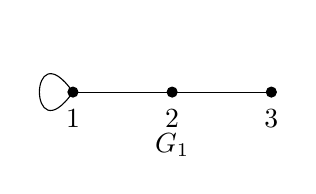
\begin{tikzpicture}[scale=.9]
  \coordinate (A) at (0,0);
  \coordinate (B) at (1.4,0);
  \coordinate (C) at (2.8,0);
  \draw (A)--(B)--(C);
  \draw (A) to[out=125,in=235,distance=1.1cm] (A);
  \filldraw (A) circle (2pt) node[below=3pt] {$1$};
  \filldraw (B) circle (2pt) node[below=3pt] {$2$};
  \filldraw (C) circle (2pt) node[below=3pt] {$3$};
  \node at (1.4,-.75) {$G_1$};
\end{tikzpicture}
\hspace{1.2cm}
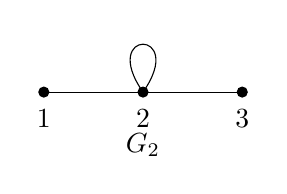
\begin{tikzpicture}[scale=.9]
  \coordinate (A) at (0,0);
  \coordinate (B) at (1.4,0);
  \coordinate (C) at (2.8,0);
  \draw (A)--(B)--(C);
  \draw (B) to[out=55,in=125,distance=1.1cm] (B);
  \filldraw (A) circle (2pt) node[below=3pt] {$1$};
  \filldraw (B) circle (2pt) node[below=3pt] {$2$};
  \filldraw (C) circle (2pt) node[below=3pt] {$3$};
  \node at (1.4,-.75) {$G_2$};
\end{tikzpicture}
\caption{Looped graphs with equal $U$-polynomials and distinct loopy
polynomials.}
\label{fig:looped-P3}
\end{figure}

Since a loop contributes a factor $y$ to the $U$-polynomial, we have
\begin{equation}\label{eq:looped-P3-U}
   U_{G_1}(\bz,y)
   =U_{G_2}(\bz,y)
   =y\bigl(z_3+2z_2z_1+z_1^3\bigr).
\end{equation}
Equivalently, $\eta_{G_1}=\eta_{G_2}$ and $\XB_{G_1}=\XB_{G_2}$.  On the
Tutte-symmetric side this is also immediate from
\begin{equation}\label{eq:XB-loop-rule}
   \XB_{G+\ell_v}(q;\bw)
   =(1+q)\XB_G(q;\bw),
\end{equation}
which is independent of the vertex carrying the loop.

Merino and Noble observed that
$U_{G_1}^{\ext}\ne U_{G_2}^{\ext}$~\cite{MN}: the extended
invariant remembers to which component the loop belongs in each spanning
subgraph.  The ordinary loopy polynomial also retains enough of this
information.  Indeed, Theorem~\ref{thm:forests-sum} gives
\begin{equation}\label{eq:looped-P3-L}
   \LL_{G_1}
   =x_3+t x_0x_2+t x_1^2+t^2x_0^2x_1,
   \qquad
   \LL_{G_2}
   =x_3+2t x_0x_2+t^2x_0^2x_1.
\end{equation}
Hence
\[
   U_{G_1}=U_{G_2}
   \qquad\text{but}\qquad
   \LL_{G_1}\ne\LL_{G_2}.
\]

\begin{example}[Loops destroy the equivalence]
\label{ex:loop-necessary}
The pair $G_1,G_2$ above has the same $U$-polynomial,
polychromate, and Tutte symmetric function, but different extended
$U$-polynomials, refined loopy polynomials, and ordinary loopy polynomials.
Thus the specialization $U^{\ext}\to U$ is already non-injective if loops are allowed, and Conjecture~\ref{conj:L-XB-equivalence} fails there as well.
\end{example}

The example also clarifies the nature of the two specializations of the common refinement.
The $U$-polynomial remembers only the \emph{total} cyclomatic number through the
global power of $y-1$, so moving a loop from one vertex to another is invisible.
The loopy specialization keeps the quantities $s-1+r$ separately for each forest component,
and can therefore remember the location of a loop indirectly, through the component that contains it.

\subsubsection{Multiple edges and the Merino--Noble problem}
\label{subsubsec:multiple-edges}

The same mechanism shows that the simplicity hypothesis in
Conjecture~\ref{conj:L-XB-equivalence} cannot be weakened to looplessness either:
multiple edges alone already destroy the equivalence.

\begin{figure}[ht]
\centering
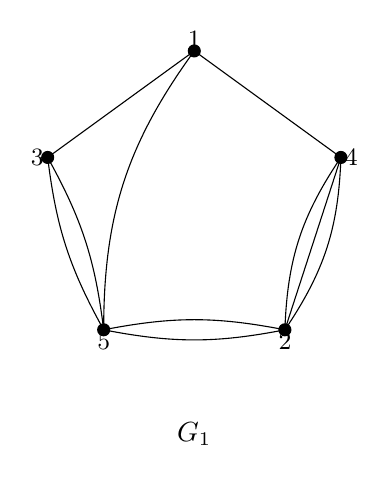
\begin{tikzpicture}[scale=1.35, every node/.style={inner sep=1.2pt}]
 \def\R{1.45}
 \foreach \nm/\ang in {a/90, b/162, c/234, d/306, e/18}
   \coordinate (\nm) at (\ang:\R);
 \draw (a) to[bend left=0] (b);
 \draw (b) to[bend left=11] (c);  \draw (b) to[bend right=11] (c);
 \draw (c) to[bend left=11] (d);  \draw (c) to[bend right=11] (d);
 \draw (d) to[bend left=16] (e);  \draw (d) -- (e); \draw (d) to[bend right=16] (e);
 \draw (e) to[bend left=0] (a);
 \draw (a) to[bend right=18] (c);
 \foreach \nm/\lab/\pos in {a/1/above, b/3/left, c/5/below, d/2/below, e/4/right}
   \filldraw[black] (\nm) circle (1.6pt) node[\pos] {\small $\lab$};
 \node at (0,-2.15) {$G_1$};
\end{tikzpicture}
\hspace{2.2cm}
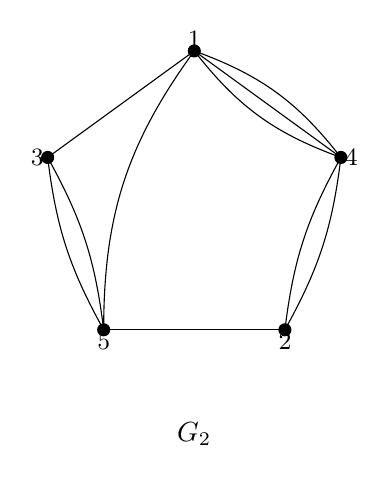
\begin{tikzpicture}[scale=1.35, every node/.style={inner sep=1.2pt}]
 \def\R{1.45}
 \foreach \nm/\ang in {a/90, b/162, c/234, d/306, e/18}
   \coordinate (\nm) at (\ang:\R);
 \draw (a) to[bend left=0] (b);
 \draw (b) to[bend left=11] (c);  \draw (b) to[bend right=11] (c);
 \draw (c) to[bend left=0] (d);
 \draw (d) to[bend left=11] (e);  \draw (d) to[bend right=11] (e);
 \draw (e) to[bend left=16] (a);  \draw (e) -- (a); \draw (e) to[bend right=16] (a);
 \draw (a) to[bend right=18] (c);
 \foreach \nm/\lab/\pos in {a/1/above, b/3/left, c/5/below, d/2/below, e/4/right}
   \filldraw[black] (\nm) circle (1.6pt) node[\pos] {\small $\lab$};
 \node at (0,-2.15) {$G_2$};
\end{tikzpicture}
\caption{Two non-isomorphic loopless graphs on five vertices and ten
edges with $\XB_{G_1}=\XB_{G_2}$ and $U_{G_1}=U_{G_2}$, but
$\LL_{G_1}\ne\LL_{G_2}$.  They share the underlying simple graph, a $5$-cycle
with one chord, and differ only in the multiplicities along the path
$5,2,4,1$.}
\label{fig:parallel-counterexample}
\end{figure}

\begin{theorem}[Solution of the Merino--Noble problem]
\label{thm:MN-solved}
There exist non-isomorphic loopless multigraphs $G_1,G_2$ with
\[
   U_{G_1}=U_{G_2}
   \qquad\text{but}\qquad
   U^{\ext}_{G_1}\ne U^{\ext}_{G_2},
\]
answering the question~\eqref{eq:MN-open-problem} of Merino and Noble.  For
the same pair
$\LL_{G_1}\ne\LL_{G_2}$ while $\XB_{G_1}=\XB_{G_2}$, so the conclusion of
Conjecture~\ref{conj:L-XB-equivalence} also fails on loopless graphs.
\end{theorem}

\begin{proof}
  Take $G_1$ and $G_2$ to be the two graphs of Figure~\ref{fig:parallel-counterexample}.
  The assertions are verified in Example~\ref{ex:parallel-necessary}.
\end{proof}

\begin{example}[An explicit pair]
\label{ex:parallel-necessary}
Let $G_1$ and $G_2$ be the two graphs of Figure~\ref{fig:parallel-counterexample}.
Both have the $5$-cycle $1,3,5,2,4$ with the chord $\{1,5\}$ as underlying simple graph, all six
underlying edges being present, and the multiplicities
\[
\begin{array}{lcccccc}
     & \{1,3\} & \{3,5\} & \{5,2\} & \{2,4\} & \{4,1\} & \{1,5\}\\[1mm]
 G_1 &   1     &    2    &    2    &    3    &    1    &    1   \\
 G_2 &   1     &    2    &    1    &    2    &    3    &    1
\end{array}
\]
Then $G_1\not\cong G_2$, and
\[
   \XB_{G_1}=\XB_{G_2},
   \qquad
   U_{G_1}=U_{G_2},
   \qquad\text{but}\qquad
   \LL_{G_1}\ne\LL_{G_2}.
\]
Indeed
\[
   \LL_{G_1}-\LL_{G_2}
   =t^3\bigl(x_3x_4-x_2x_5\bigr)
    +t^4\bigl(x_3^2-x_2x_4\bigr)
    +t^5\bigl(x_1x_4-x_2x_3\bigr)
    +t^6\bigl(x_0x_1x_3-x_0x_2^2\bigr),
\]
so these graphs are separated already by the distribution of the statistic
$|E(T)|+\eps_F(T)$ between the components of a
two-component spanning forest.  They also have the same Tutte polynomial and
the same degree sequence $(3,3,4,5,5)$.

Since $\widehat{\LL}\leftrightarrow U^{\ext}$ by
Theorem~\ref{thm:refined-extended-U}, the pair simultaneously solves the
Merino--Noble problem~\eqref{eq:MN-open-problem}:
$U_{G_1}=U_{G_2}$ while
$U^{\ext}_{G_1}\ne U^{\ext}_{G_2}$.  A single coefficient
already witnesses the latter:
\[
   [z_{2,1}z_{3,0}]\,U^{\ext}_{G_1}=19
   \ne
   17=[z_{2,1}z_{3,0}]\,U^{\ext}_{G_2},
\]
that is, $G_1$ and $G_2$ have different numbers of spanning subgraphs with two
components, one of order $2$ and cyclomatic number $1$, the other of order
$3$ and cyclomatic number $0$.  All the assertions above
were checked exactly over $\ZZ$, by two independent implementations, and $G_1\not\cong G_2$
was verified over all $120$ relabelings.
\end{example}

We found this pair by an exhaustive search over loopless multigraphs with small
vertex count and bounded edge multiplicity, using the same fingerprints as in Section~\ref{sec:the-computation}.
Here $e_G(S)$ simply counts edges with multiplicity, and nothing else in the algorithm changes.
Writing $\mu$ for the maximum multiplicity allowed, the counts of connected loopless
multigraphs and of their nontrivial collision classes are as follows.

\begin{center}
\begin{tabular}{ccrrr}
\toprule
$n$ & $\mu$ & multigraphs & $\LL$-classes & $\XB$-classes\\
\midrule
$4$    & $9$    & $45\,210$    & $0$   & $0$\\
$5$    & $2$    & $712$        & $0$   & $0$\\
$5$    & $3$    & $10\,364$    & $0$   & $12$\\
$5$    & $4$    & $88\,985$    & $0$   & $58$\\
$5$    & $5$    & $530\,657$   & $0$   & $166$\\
$5$    & $6$    & $2\,431\,555$& $0$   & $360$\\
$6$    & $2$    & $24\,576$    & $15$  & $30$\\
$6$    & $3$    & $1\,590\,368$& $500$ & $1\,130$\\
$6$    & $4$    & $43\,477\,490$& $4\,848$ & $10\,164$\\
$7$    & $2$    & $2\,275\,616$& $1\,213$ & $1\,469$\\
\bottomrule
\end{tabular}
\end{center}

The ranges are nested --- the rows with the same $n$ and smaller $\mu$ are
contained in the largest one for that $n$, so the row totals must not be
added --- and the graphs covered are those of the four maximal rows $(4,9)$, $(5,6)$, $(6,4)$ and $(7,2)$.
These rows contain $48\,229\,871$ connected loopless multigraphs in all.
Every $\LL$-class found is a pair.  Two of the
$\XB$-classes at $(6,4)$ have three members and all others are pairs.

Only one part of this table carries genuinely new distinguishing-power information.
It is worth separating what is observed from what is forced.  The equivalences
$U\leftrightarrow\eta\leftrightarrow \XB$ hold for all graphs, loops and
multiple edges included~\cite{NW,Sar,MN,Nob}, so the agreement of the $U$- and
$\XB$-columns is a check on the implementation rather than a new result.  What
is observed is that throughout the tested range
\[
   \LL_G=\LL_H
   \quad\Longrightarrow\quad
   \widehat{\LL}_G=\widehat{\LL}_H .
\]
Since $\widehat{\LL}_G$ determines $\XB_G$ by
Corollary~\ref{cor:refined-L-determines-XB}, this forces
$\LL_G=\LL_H\Rightarrow \XB_G=\XB_H$ throughout the same range.  The
refinement is strict because Theorem~\ref{thm:MN-solved} gives pairs with
equal $\XB$ but distinct $\LL$.  Thus the implication
$U_G=U_H\Rightarrow\LL_G=\LL_H$ fails globally on loopless graphs,
whereas the reverse implication holds for every multigraph in the search and
remains open in general, see Problem~\ref{prob:extended}.  In other words,
passing from $\widehat{\LL}$ to $\LL$ lost no distinguishing
power on any of the $48\,229\,871$ connected loopless multigraphs tested, even
though the specialization $U^{\ext}\to U$ demonstrably does.

The surviving loopy specialization retains one number per forest component.
That number is not an arbitrary way to compress the pair
$\bigl(|V(T)|,\eps_F(T)\bigr)$ into a single index.
By Theorem~\ref{thm:polyhedral-parking-cells} it is the length of an interval
factor in the box~\eqref{eq:terminal-box}.  Thus the specialization for which
we observed no loss of distinguishing power on loopless multigraphs is also
the one with a direct polyhedral meaning.  The polyhedral interpretation is
independent of the computation above and
provides further evidence that the loopy specialization is the natural one.


The pair of Theorem~\ref{thm:MN-solved} has five vertices and ten edges.
It has the smallest vertex count found in our
bounded-multiplicity search.
There is no counterexample on four vertices with all multiplicities at most
nine, and none on five vertices with all multiplicities at most two, while
examples appear as soon as $\mu=3$ is allowed.  In the number of edges it is
not smallest.  A connected loopless multigraph with at most eight edges has at
most nine vertices, so that range is finite.  An exhaustive check over all
connected loopless multigraphs with at most nine edges---bounding the number of
edges rather than the multiplicity, and again exact over $\ZZ$---shows
that none with at most eight edges is a counterexample, whereas nine-edge
counterexamples do exist, on six, seven, eight and nine vertices.  The one
remaining case, a tree on ten vertices, is simple and hence separated by
Proposition~\ref{cor:forest-L-X}.  This check is the script \texttt{min\_edges.py}
of~\cite{code}.  The nine-edge examples have maximum
multiplicity two, so one of them already occurs in the $(6,2)$ row of the table
above.  We state Theorem~\ref{thm:MN-solved} with the five-vertex pair because
the number of vertices is the parameter that governs the search.

There is a structural reason to expect this asymmetry.  The two specializations of
the common refinement discard different things.
Passing from $U^{\ext}$ to $U$ replaces the multiset of pairs $\bigl(|V(D)|,\nu(D)\bigr)$
by the multiset of orders together with the \emph{total} cyclomatic number $\sum_D\nu(D)$,
so all record of how the cyclomatic number is distributed among the components is lost.
Passing from $\widehat{\LL}$ to $\LL$ instead retains one number per component,
the sum $|E(T)|+\eps_F(T)$.
A per-component statistic is a good deal more informative than a global total,
and the counterexample above is exactly of this shape: the terms $x_2x_5$ and $x_3x_4$ of
Example~\ref{ex:parallel-necessary} have the same total but different distributions.

Thus loops and multiple edges are obstructions of the same kind, and simplicity is a necessary hypothesis in
Conjecture~\ref{conj:L-XB-equivalence} rather than a convenience.
We emphasize that neither obstruction bears on the simple-graph case: both the equivalence conjecture
and the simple-graph version of the Merino--Noble problem remain open there, and
Proposition~\ref{prop:computational-evidence} verifies both through eleven vertices.

\section{Structural evidence}
\label{sec:structural-evidence}
Beyond the exhaustive verification of Section~\ref{sec:extended-U},
several structural results bear on the conjecture.
The first is about the collision classes themselves: they are closed under complementation and
under joins, which accounts for much of the shape of the census in Section~\ref{sec:extended-U}.
The second recasts the implication from $U$ to $L$
as a compatibility problem for block transforms, potentially weaker than recovering $U^\ext$ from $U$.
The third reduces the conjecture for connected unicyclic simple graphs to an injectivity
question for a rooted tree invariant, and settles it unconditionally when the cycle is long relative
to the graph.
The fourth shows that the loopy polynomial and the Tutte symmetric function satisfy
a common modular four-term relation.

\subsection{Complementation and joins}
\label{subsec:complementation}
It is convenient to shift the edge variable.
Write
\begin{equation}\label{eq:XB-tilde}
  \widetilde{\XB}_G(t;\bw):=\XB_G(t-1;\bw) = \sum_{\kp}t^{\,b_G(\kp)}\bw^{\kp},
\end{equation}
where $\kp$ runs over the colorings of $V(G)$ and $b_G(\kp)$ is the number of monochromatic edges of $\kp$.

\begin{proposition}[Complementation]\label{prop:XB-complement}
$\XB_G$ determines $\XB_{\overline G}$, and the passage from one to the other is
invertible.  Explicitly, for every monomial $\bw^{\alpha}$,
\[
   [\bw^{\alpha}]\,\widetilde{\XB}_{\overline G}(t)
   \;=\;
   t^{\,c(\alpha)}\;[\bw^{\alpha}]\,\widetilde{\XB}_{G}(t^{-1}),
   \qquad
   c(\alpha)=\sum_i\binom{\alpha_i}{2}.
\]
\end{proposition}

\begin{proof}
For a fixed coloring $\kp$ the color classes partition $V$, and every
pair inside a class is an edge of exactly one of $G$, $\overline G$.  Hence
$b_{\overline G}(\kp)=c(\alpha)-b_G(\kp)$, where $\alpha$ is the
multiset of color-class sizes.  Summing over the colorings contributing to
$\bw^{\alpha}$ gives the displayed identity.  The transformation is its
own inverse up to the substitution $t\mapsto t^{-1}$, so it is invertible.
\end{proof}

Joining a fixed graph to both members of a collision therefore preserves it,
and nothing is lost in the other direction either.

\begin{corollary}[Joins]\label{cor:join-equivalence}
Let $J$ be any graph, and write $G\vee J$ for the graph join.  Then for all
$G_1,G_2$,
\begin{equation}\label{eq:join-equivalence}
   \XB_{G_1\vee J}=\XB_{G_2\vee J}
   \quad\Longleftrightarrow\quad
   \XB_{G_1}=\XB_{G_2}.
\end{equation}
Thus joining $J$ maps the collision classes of $\XB$ bijectively to collision
classes of $\XB$.
\end{corollary}

\begin{proof}
The complement of a join is the disjoint union of the complements,
\[
  \overline{G\vee J}=\overline G\sqcup\overline J,
\]
so multiplicativity gives
\[
   \XB_{\overline{G_i\vee J}}
   =\XB_{\overline{G_i}}\cdot \XB_{\overline J},
   \qquad i=1,2.
\]
By Proposition~\ref{prop:XB-complement} the left-hand sides are equal if and
only if $\XB_{G_1\vee J}=\XB_{G_2\vee J}$, and $\XB_{\overline{G_1}}=
\XB_{\overline{G_2}}$ if and only if $\XB_{G_1}=\XB_{G_2}$.  Since all
coefficients of $\XB_{\overline J}$ are nonnegative and its constant term is
$1$, it is a nonzero element of the integral domain
$\QQ[q,p_1,p_2,\ldots]$ and may be canceled.
\end{proof}

\begin{remark}
 \label{rem:complementation}
Proposition~\ref{prop:XB-complement} and Corollary~\ref{cor:join-equivalence}
account for three further features of the computation.

\emph{(a) Closure.}  The transformation of the proposition is invertible, so
$\XB_G=\XB_H$ implies $\XB_{\overline G}=\XB_{\overline H}$: the collision classes
of $\XB$ are closed under complementation.  Since the computation shows that
the $\LL$- and $\XB$-classes coincide for $n\le11$, the same closure holds for
the loopy polynomial in that range, and we have verified it directly on all
$73$ classes with $n\le9$.  More generally
Conjecture~\ref{conj:L-XB-equivalence} implies the class-level form of
Problem~\ref{prob:complement}, so a counterexample to the latter would refute
the former as well.

\emph{(b) Joins.}
By Corollary~\ref{cor:join-equivalence}, joining a fixed graph carries
collision classes to collision classes bijectively.  In particular, if $G_1$
and $G_2$ with $n$ vertices and $m$ edges collide, then so do their cones
$K_1\vee G_1$ and $K_1\vee G_2$, with $n+1$ vertices and $m+n$ edges.  More
generally, a collision class is obtained from a nontrivial join exactly when
its members have disconnected complement.  This
gives a check on the search that does not pass through the fingerprints: all
eight classes at $n=8$ reappear in the $n=9$ list at $21\le m\le23$, and all
$1\,285$ connected classes at $n=10$ reappear in the $n=11$ list at $m+10$.

At $n=11$, joins account for $1\,447$ of the $22\,499$ connected collision
classes.  Of these, $1\,366$ are cones, i.e.\ have a $K_1$ join factor.  They
are obtained by coning the $1\,366$ nontrivial collision classes on arbitrary
ten-vertex simple graphs: the $1\,285$ connected classes and $81$ disconnected
classes.  By unique factorization, the latter decompose as
$81=65+8+8$: they are $G_0\sqcup K_1$ with $G_0$ one of the $65$ classes at
$n=9$, or $G_0\sqcup2K_1$ or $G_0\sqcup K_2$ with $G_0$ one of the $8$
classes at $n=8$.  The other $81=65+8+8$ join-generated classes at $n=11$
have no $K_1$ factor: $65$ are $G_0\vee\overline{K_2}$ with $G_0$ a class at
$n=9$, and $8$ each are $G_0\vee\overline{K_3}$ and
$G_0\vee\overline{P_3}$ with $G_0$ a class at $n=8$.
Thus $1\,447=1\,366+81$.  The remaining $21\,052=22\,499-1\,447$ classes have
connected complement and are not produced by a nontrivial join.


\emph{(c) Edge ranges.}  Complementation sends a class at $m$ to a class at
$\binom n2-m$, so the observed ranges would be symmetric were it not that the
search sees connected simple graphs only.
For $n=8,9,11$ they are symmetric: $13$--$15$, $13$--$23$, $13$--$42$.
The exception at $n=10$ is instructive. There the range is $14$--$32$ and
no connected simple graph with $13$ edges lies in a collision class, so complementing
the classes with $m=32$ must produce
collisions at $m=45-32=13$ between \emph{disconnected} simple graphs, invisible to the search.
That is precisely what happens, and the count is fully accounted for:
there are three classes with $(n,m)=(10,32)$, and their complements are
\[
   F\sqcup 2K_1 \ \ \text{for each of the two classes $F$ at }(8,13),
   \quad
   F\sqcup K_1 \ \ \text{for the single class $F$ at }(9,13).
\]
By multiplicativity and unique factorization
(Corollary~\ref{cor:L-component-factorization}), a disconnected simple graph
on ten vertices with thirteen edges lies in a collision class if and only if
its nontrivial components do.  There is no other way to assemble one: there
are no collisions at $(8,12)$ or at $(7,13)$, and none at all below eight
vertices.  Hence $3=2+1$, with nothing unexplained.  The asymmetry is thus a
real feature of the connected-graph data rather than a gap in it, and it
illustrates Corollary~\ref{cor:connected-reduction}: restricting to connected
graphs loses no information, but it does relocate some of it.
\end{remark}

\subsection{A blockwise reformulation}
\label{subsec:block-transform}
We next isolate one direction of Conjecture~\ref{conj:L-XB-equivalence} in a
form that does not attempt to reconstruct the full extended $U$-polynomial.
The point is that $\XB_G$ records, for each block-size profile, a symmetrized
sum of products of connected-block polynomials, whereas $\LL_G$ requires
applying a size-dependent linear transform to each block polynomial before
taking the corresponding symmetrized sum.  Thus the implication
\[
   U_G=U_H\quad\Longrightarrow\quad \LL_G=\LL_H
\]
becomes a concrete compatibility problem for these block transforms, and is potentially weaker
than recovering $U_G^{\ext}$ from $U_G$.  We now make this formulation precise.

Let $\Pi(V)$ denote the set of set partitions of a finite set $V$,
and let $\lambda(\pi)$ be the integer partition formed by the block sizes of $\pi$.
For a graph $H$, write $\ST(H)$ for its set of spanning trees, and write $\eps_H(\tau)$
for the external activity of a spanning tree $\tau$, computed in $H$ with the inherited edge order.

For a nonempty vertex set $B\subseteq V(G)$ define
\begin{equation}\label{eq:connected-block-polynomial}
 \cC_G(B;q) := \sum_{\substack{A\subseteq E(G[B])\\(B,A)\text{ connected}}} q^{|A|}.
\end{equation}
For a singleton we put $\cC_G(B;q)=1$.  Grouping the spanning-subgraph
expansion~\eqref{eq:XB-subgraph} according to its connected-component partition gives
\begin{equation}\label{eq:XB-connected-block-expansion}
   \XB_G(q;\bw)
   =
   \sum_{\pi\in\Pi(V(G))}
   \left(\prod_{B\in\pi}\cC_G(B;q)\right)
   \prod_{B\in\pi}p_{|B|}.
\end{equation}
For an integer partition $\lambda\vdash n$, set
\begin{equation}\label{eq:S-lambda-definition}
   S^G_\lambda(q):=[p_\lambda]\XB_G(q;\bw).
\end{equation}
Then
\begin{equation}\label{eq:S-lambda-blocks}
   S^G_\lambda(q)
   =
   \sum_{\substack{\pi\in\Pi(V(G))\\\lambda(\pi)=\lambda}}
   \prod_{B\in\pi}\cC_G(B;q).
\end{equation}
Thus $\XB_G$, or equivalently $U_G$ and $\eta_G$, remembers for every block
profile $\lambda$ a symmetrized sum of products of the connected-block
polynomials.

When $G[B]$ is connected and $|B|=s$, the polynomial $\cC_G(B;q)$ is divisible by $q^{s-1}$,
so it belongs to $q^{s-1}\QQ[1+q]$.  For $s\ge 1$, define a linear map
\begin{equation}\label{eq:block-transform}
   \fT_s:q^{s-1}\QQ[1+q]
   \longrightarrow
   \QQ[x_0,x_1,\ldots]
\end{equation}
by
\begin{equation}\label{eq:block-transform-on-basis}
   \fT_s\bigl(q^{s-1}(1+q)^r\bigr)
   =x_{s-1+r},
   \qquad r\ge 0.
\end{equation}
For $s=1$ this includes $\fT_1(1)=x_0$.

\begin{proposition}\label{prop:block-transform-L}
For every simple graph $G$,
\begin{equation}\label{eq:L-block-transform}
   \LL_G(1,\bx)
   =
   \sum_{\pi\in\Pi(V(G))}
   \prod_{B\in\pi}
   \fT_{|B|}\bigl(\cC_G(B;q)\bigr).
\end{equation}
\end{proposition}

\begin{proof}
Fix an edge order.  If $|B|=s$, the activity-interval decomposition
\eqref{eq:activity-intervals}, applied to connected spanning subgraphs of $G[B]$, gives
\begin{equation}\label{eq:block-C-activity}
   \cC_G(B;q)
   =
   \sum_{\tau\in\ST(G[B])}
   q^{s-1}(1+q)^{\eps_{G[B]}(\tau)},
\end{equation}
where the sum is empty when $G[B]$ is disconnected.  Hence
  \begin{equation}\label{eq:tau-sum}   \fT_s\bigl(\cC_G(B;q)\bigr)
   =
   \sum_{\tau\in\ST(G[B])}
   x_{s-1+\eps_{G[B]}(\tau)}.
 \end{equation}
A spanning forest of $G$ is the same as a set partition $\pi$ of $V(G)$
 with a spanning tree of $G[B]$ for every block $B\in\pi$.  External
activity is computed independently inside these components.  Multiplying~\eqref{eq:tau-sum}
 over the blocks and summing over $\pi$ therefore gives exactly the forest expansion of $\LL_G(1,\bx)$.
\end{proof}

Thus the ordinary invariant and the loopy invariant are obtained from the
same family of connected-block polynomials by two different operations:
$\XB_G$ first forms symmetrized products and records them through the
power-sum basis, while $\LL_G$ first applies a size-dependent linear transform
to each block polynomial and then forms the same symmetrized products.  This
leads to a concrete form of one half of the main conjecture.

\begin{problem}[Block-transform problem]
\label{prob:block-transform}
Show that for simple graphs $G$ and $H$ on the same number of vertices,
\[
   S^G_\lambda(q)=S^H_\lambda(q) \qquad\text{for every integer partition }\lambda
\]
implies
\begin{equation}\label{eq:block-transform-problem}
  \sum_{\pi\in\Pi(V(G))} \prod_{B\in\pi}\fT_{|B|}
  \bigl(\cC_G(B;q)\bigr) = \sum_{\pi\in\Pi(V(H))}
   \prod_{B\in\pi}\fT_{|B|} \bigl(\cC_H(B;q)\bigr).
\end{equation}
By~\eqref{eq:XB-connected-block-expansion} and
Proposition~\ref{prop:block-transform-L}, this is precisely the implication
$\XB_G=\XB_H\Rightarrow\LL_G=\LL_H$ in Conjecture~\ref{conj:L-XB-equivalence}.
\end{problem}

The first partition types in this problem are automatic.  For example, if
$\lambda=(s,1^{n-s})$, then
\begin{equation}\label{eq:one-block-component}
   S^G_{(s,1^{n-s})}(q)
   =
   \sum_{\substack{B\subseteq V(G)\\|B|=s}}
   \cC_G(B;q),
\end{equation}
and linearity of $\fT_s$ determines the corresponding part of $\LL_G(1,\bx)$.
Thus the first possible obstruction occurs only when the component partition has at least two nonsingleton blocks.
In that case $\XB_G$ knows a sum of products of block polynomials, whereas $\LL_G$
requires the sum of the products after different size-dependent linear maps have been applied.
For arbitrary polynomial-valued set functions this information is not sufficient, as the following example shows.
Thus any proof must use the special graphical origin of the block polynomials.

\begin{example}[Symmetrized sums do not control transformed sums]
\label{ex:block-transform-insufficient}
Let $V=\{1,2,3,4\}$ and let $f,g$ be $\ZZ[q]$-valued functions on the nonempty subsets
of $V$ with $f(B)=g(B)$ for all $|B|\ne 2$, with $f(\{v\})=g(\{v\})=1$, \ $f(B)= 0$ for $|B|=2$, and with
\[
  g(12)=g(34)=q, \ \  g(13)=1,\ \ g(24)=-q^{2}, \ \ g(14)=0,\ \ g(23)=q^{2}-2q-1 .
\]
Then $f$ and $g$ have the same symmetrized sums for every partition type:
the only types involving two-element blocks are $(2,1^2)$ and $(2,2)$, and
\[
   \sum_{|B|=2}g(B)=0,
   \qquad
   g(12)g(34)+g(13)g(24)+g(14)g(23)=q^{2}-q^{2}+0=0 .
\]
Now let $\fT_2=[q]$ extract the coefficient of $q$, and let $\fT_s$ be the identity for $s\ne2$.
These are linear, but not ring maps, and
\[
   \sum_{\pi\text{ of type }(2,2)}\prod_{B\in\pi}\fT_2\bigl(g(B)\bigr)
   =1\cdot1+0\cdot0+0\cdot(-2)=1,
\]
whereas the same sum for $f$ is $0$, so the two transformed sums differ.
(The type $(2,1^2)$ case still agrees, since
$\sum_{|B|=2}\fT_2(g(B))=0$.)  Thus the failure is exactly at the first type with two nonsingleton blocks,
and nothing about the symmetrized data alone can rule it out.
\end{example}

This formulation is complementary to the simple-graph recovery question left open after
Theorem~\ref{thm:MN-solved}.  Recovering $U_G^{\ext}$ from $U_G$ on simple graphs would prove
the implication in the block problem, but the block problem asks for less:
it seeks only the particular diagonal specialization needed to recover $\LL_G$.


\subsection{Unicyclic graphs: a pointed-forest reduction}
\label{subsec:unicyclic}

The equivalence conjecture is automatic for forests by
Proposition~\ref{cor:forest-L-X}.  The next natural case is that of connected
unicyclic graphs.  The activity expansion reduces this case to a single
concrete question about rooted trees, which we verify computationally in a
wide range and which we are able to prove outright for a substantial
subclass.

Throughout this subsection $G$ is a connected simple unicyclic graph with $n(G)=n$ and
the unique cycle $C\subseteq G$ of length
$   g:=|V(C)|\ \ge\ 3.$
Since $G$ is connected and unicyclic,
$m(G)=n$.  Fix an ordering of $E(G)$ and let $e_0$ be the least edge of $C$.
The order of the remaining edges will not matter.

\begin{lemma}\label{lem:unicyclic-activity}
For every spanning forest $F$ of $G$ one has $\eps(F)\in\{0,1\}$, and
\begin{equation}\label{eq:unicyclic-active}
   \eps(F)=1
   \quad\Longleftrightarrow\quad
   F\cap E(C)=E(C)\setminus\{e_0\}.
\end{equation}
In that case all vertices of $C$ lie in a single component $T_*(F)$ of $F$, and
\[
   \eps_F(T_*(F))=1,
   \qquad
   \eps_F(T)=0
   \quad\text{for }T\ne T_*(F).
\]
\end{lemma}

\begin{proof}
Every edge outside $C$ is a bridge of $G$.  If such an edge is omitted from a
spanning forest, its endpoints lie in different components, so it is not externally active.

Now let $e\in E(C)\setminus F$.  The endpoints of $e$ are connected in $F$ if
and only if all the other edges of $C$ belong to $F$.  Thus an omitted cycle
edge can be externally active only when it is the unique omitted edge of $C$,
and then the unique cycle of $F\cup\{e\}$ is $C$ itself, so $e$ is externally
active precisely when $e=e_0$.  This proves~\eqref{eq:unicyclic-active}.
When it holds, $C-e_0\subseteq F$ is a spanning path on the vertices of
$C$, so all cycle vertices lie in one component of $F$, and the unique active
edge $e_0$ is assigned to that component.
\end{proof}

By~\eqref{eq:activity-from-monomial} the total activity of a forest is already visible in its $\bx$-monomial.
Thus the active and inactive parts of $\LL_G$  can be separated without using the $t$-grading,
and so we will with $\LL_(1,\bx)$ from now on.

Introduce the \emph{inactive polynomial}
\begin{equation}\label{eq:unicyclic-inactive}
   F_G(\bz) := \sum_{\substack{F\in\cF(G)\\ \eps(F)=0}} \prod_{T\in c(F)} z_{|V(T)|},
\end{equation}
and, for the active forests, a second family of variables
$\bz^\bullet=(z_1^\bullet,z_2^\bullet,\ldots)$ recording the component
that carries the cycle:
\begin{equation}\label{eq:unicyclic-pointed}
   B_G^\bullet(\bz;\bz^\bullet) := \sum_{\substack{F\in\cF(G)\\ \eps(F)=1}}
   z^\bullet_{|V(T_*(F))|} \prod_{\substack{T\in c(F)\\T\ne T_*(F)}} z_{|V(T)|},
 \qquad  B_G(\bz):=B_G^\bullet(\bz;\bz).
\end{equation}
Although the definition refers to $e_0$, the polynomial $B_G^\bullet$ does not
depend on that choice.  Indeed, by Lemma~\ref{lem:unicyclic-activity} an
active forest is $C-e_0$ together with an arbitrary subset of the bridges of
$G$, and $C-e$ is a spanning path on $V(C)$ for \emph{every} $e\in E(C)$.
Hence the vertex sets of the resulting components are the same whichever cycle
edge is removed.

\begin{proposition}\label{prop:unicyclic-two-specializations}
For a connected unicyclic simple graph $G$, we have
\begin{equation}\label{eq:unicyclic-U-decomposition}
   U_G(\bz,y)
   =
   F_G(\bz)+y\,B_G(\bz),
\end{equation}
\begin{equation}\label{eq:unicyclic-L-decomposition}
   \LL_G(1,\bx)
   =
   \left.F_G(\bz)\right|_{z_s=x_{s-1}}
   +
   \left.B_G^\bullet(\bz;\bz^\bullet)\right|_{z_s=x_{s-1},\ z_s^\bullet=x_s}.
\end{equation}
Moreover $U_G$ and $\LL_G$ each determine $n$, $g$ and $F_G$.
\end{proposition}

\begin{proof}
Formula~\eqref{eq:unicyclic-U-decomposition} followsfrom~\eqref{eq:U-forest} and
Lemma~\ref{lem:unicyclic-activity}: an inactive forest contributes $\ds \prod_T z_{|V(T)|}$
and an active one contributes $\ds y\prod_T z_{|V(T)|}$ obtained from~\eqref{eq:unicyclic-pointed}
by forgetting the distinguished component.

For $\LL_G(1,\bx)$ an inactive component $T$ contributes $x_{|V(T)|-1}$.
In an active forest the distinguished component has activity one and contributes $x_{|V(T_*)|}$,
while every other component contributes $x_{|V(T)|-1}$.  This gives~\eqref{eq:unicyclic-L-decomposition}.

Both invariants determine the ordinary Tutte polynomial,
and for a connected unicyclic graph
\begin{equation}\label{eq:unicyclic-Tutte}
   T_G(X,Y)=X^{n-g}\bigl(X^{g-1}+X^{g-2}+\cdots+X+Y\bigr),
\end{equation}
since the $n-g$ edges outside $C$ are bridges.  Hence each determines $n$ and
$g$.  Finally $F_G=\left.U_G\right|_{y=0}$, while on the loopy side the
inactive monomials are recognized by~\eqref{eq:activity-from-monomial} and the
relabeling $x_{s-1}\mapsto z_s$ returns the same polynomial.
\end{proof}

The content of the unicyclic case is therefore exactly the following.

\begin{corollary}\label{cor:unicyclic-reduction}
Let $G$ and $G'$ be connected unicyclic simple graphs.  Then
\begin{align}
   U_G=U_{G'}
   &\iff
   n=n',\ g=g',\ F_G=F_{G'}\ \text{ and }\ B_G=B_{G'},
   \label{eq:unicyclic-U-iff}\\
   \LL_G=\LL_{G'}
   &\iff
   n=n',\ g=g',\ F_G=F_{G'}\ \text{ and }\
   \left.B_G^\bullet\right|_{z_s^\bullet=z_{s+1}}
   =\left.B_{G'}^\bullet\right|_{z_s^\bullet=z_{s+1}} .
   \label{eq:unicyclic-L-iff}
\end{align}
The two invariants therefore differ only in the way the distinguished
component of an active forest is forgotten: $U_G$ substitutes
$z^\bullet_s\mapsto z_s$, whereas $\LL_G$ substitutes
$z^\bullet_s\mapsto z_{s+1}$.
\end{corollary}

\begin{proof}
Immediate from Proposition~\ref{prop:unicyclic-two-specializations}, after
relabeling $x_i\mapsto z_{i+1}$ in~\eqref{eq:unicyclic-L-decomposition}.
\end{proof}

There is some redundancy in the inactive part.  For every fixed subset of the
bridges of $G$ there are exactly $g$ forests containing $g-1$ edges of $C$,
one for each choice of the omitted cycle edge, and they all have the same
component vertex sets.  Exactly one of them, the one omitting $e_0$, is
active.  Hence
\begin{equation}\label{eq:unicyclic-inactive-splitting}
   F_G(\bz)=(g-1)\,B_G(\bz)+F^{\ge 2}_G(\bz),
\end{equation}
where $F^{\ge 2}_G$ collects the forests omitting at least two cycle edges.
Thus the unpointed active contribution already sits, with multiplicity $g-1$,
inside the inactive part.  The unresolved issue is not the unpointed component
partition, but the identification of the component containing the cycle.

\subsubsection*{A rooted-tree reformulation}

Collapse the cycle $C$ to a single vertex $\rho$ and discard the cycle edges.
The result is a rooted tree $(H,\rho)$ with $n_H:=|V(H)|=n-g+1 $ vertices.
By Lemma~\ref{lem:unicyclic-activity}, the active forests of $G$ are exactly the sets
\[
F_J:=(C-e_0)\cup J \quad \text{with} \quad J\subseteq E(H).
\]
If $R_J$ is the
component of $(V(H),J)$ containing the root $\rho$, the distinguished component $T_*$ of $F_J$
satisfies $|V(T_*)|=g-1+|V(R_J)|$, while every other component has the same
size in $G$ as in $H$.  Accordingly, put
\begin{equation}\label{eq:root-shift-polynomial}
   \Psi_{H,g}(\bz)
   :=
   \sum_{J\subseteq E(H)}
      z_{\,g-1+|V(R_J)|}
      \prod_{\substack{D\in c(J)\\D\ne R_J}} z_{|V(D)|}.
\end{equation}
Then
\begin{equation}\label{eq:unicyclic-active-rooted}
   B_G=\Psi_{H,g},
   \qquad
   \left.B_G^\bullet\right|_{z^\bullet_s=z_{s+1}}=\Psi_{H,g+1},
\end{equation}
so Corollary~\ref{cor:unicyclic-reduction} says that, given the common data
$(n,g,F_G)$, the comparison of $U_G$ with $\LL_G$ is precisely the comparison
of $\Psi_{H,g}$ with $\Psi_{H,g+1}$.

Both are specializations of the \emph{rooted $U$-polynomial} of the rooted tree $(H,\rho)$,
\begin{equation}\label{eq:rooted-U}
 \Omega_H(w;\bz)    :=
 \sum_{J\subseteq E(H)} w^{\,|V(R_J)|}
     \prod_{\substack{D\in c(J)\\D\ne R_J}} z_{|V(D)|}
\end{equation}
introduced by Aliste-Prieto, de Mier and Zamora~\cite{ADZ},
which records the size of the root
component separately from the sizes of the remaining components and which
determines the rooted tree up to isomorphism~\cite[Theorem~9]{ADZ}.
The corresponding statement for the rooted
polychromate is due to Bollob\'as and Riordan~\cite{BR}, who introduced that
invariant for this purpose.  By construction
\begin{equation}\label{eq:Psi-from-Omega}
   \Psi_{H,g}
   =
   \left.\Omega_H(w;\bz)\right|_{w^a\mapsto z_{g-1+a}},
\end{equation}
so $\Psi_{H,g}$ is a specialization of $\Omega_H$, a priori a strictly weaker
invariant.  The difficulty in the unicyclic case is therefore not
reconstruction from the fully pointed rooted polynomial.  It is whether the two
unpointings $w^a\mapsto z_{g-1+a}$ and $w^a\mapsto z_{g+a}$ lose the same information.
%
We conjecture that in fact neither loses any.

\begin{conjecture}[Root injectivity]\label{conj:root-injectivity}
For every $g\ge 3$, the map $H\mapsto \Psi_{H,g}$ is injective on rooted trees
with a fixed number of vertices.
\end{conjecture}

\begin{proposition}\label{prop:root-injectivity-implies}
Conjecture~\ref{conj:root-injectivity} implies the equivalence conjecture for
connected unicyclic simple graphs.
\end{proposition}

\begin{proof}
Let $G,G'$ be connected unicyclic simple graphs and suppose $U_G=U_{G'}$.  By
Corollary~\ref{cor:unicyclic-reduction} we have $n=n'$, $g=g'$,
$F_G=F_{G'}$ and $\Psi_{H,g}=\Psi_{H',g}$, where $H,H'$ are the associated rooted
trees, both on $n_H=n-g+1$ vertices.  By
Conjecture~\ref{conj:root-injectivity}, $H\cong H'$ as rooted trees, whence
$\Psi_{H,g+1}=\Psi_{H',g+1}$, and \eqref{eq:unicyclic-L-iff} gives
$\LL_G=\LL_{G'}$.  The converse is identical with the roles of $g$ and $g+1$
interchanged.
\end{proof}

The rooted tree $H$ does not by itself determine $G$: collapsing the cycle forgets
how the attached branches are distributed among the cycle vertices and their cyclic arrangement.
This causes no problem in the preceding argument, because the inactive polynomial $F_G$
is retained separately as common data.
The proof does not require that this attachment information be reconstructed from $H$ alone.

\begin{remark}[Computational evidence, and sharpness at $g=2$]
\label{rem:g-two-fails}
Only a finite range of $g$ has to be tested.
For a rooted tree $H$ on $N$ vertices the case $g\ge N$ is automatic:
in every monomial of $\Psi_{H,g}$ the root-component factor has index at least $g$,
whereas every other factor has index at most $N-1$, so the root factor
is uniquely identifiable and $\Psi_{H,g}$ recovers $\Omega_H$.
It therefore suffices to test $3\le g\le N-1$.

We have verified Conjecture~\ref{conj:root-injectivity} exhaustively for all
rooted trees with at most $13$ vertices: for every such tree and every $g$ in that range,
no two rooted trees of the same order have equal $\Psi_{H,g}$.
The counts of rooted trees involved are
$1,2,4,9,20,48,115,286,719,1842,4766,12486$ for $2\le n_H\le13$.  In particular,
by Proposition~\ref{prop:root-injectivity-implies}, the above
computation implies that the equivalence conjecture holds for every connected
unicyclic simple graph with $ n-g+1\le13,$
and hence for every connected unicyclic simple graph on at most $15$ vertices.

The hypothesis $g\ge 3$ cannot be dropped.  For $g=2$ the map $H\mapsto \Psi_{H,2}$
is not injective: there is one colliding pair of rooted trees on $8$ vertices
and four on $11$ vertices.  Since a cycle in a simple graph has length at
least three, the case in which the statement fails is exactly the one that cannot arise here.
\end{remark}

\subsubsection*{Toward a proof}

The obstruction to recovering the pointing from $\Psi_{H,g}$ is entirely local: a
monomial of $\Psi_{H,g}$ is ambiguous only if two of its factors could play the
role of the distinguished one, that is, only if it has two factors of index at
least $g$.  This cannot happen when the monomial has many factors.

\begin{proposition}[High-factor terms]\label{prop:unambiguous-terms}
  Let $M$ be a monomial of degree $p$ occurring in $\Psi_{H,g}$.
  If
\[
   p\ \ge\ n_H-g+2,
\]
then $M$ has exactly one factor of index at least $g$, namely the one contributed by the root component.
\end{proposition}

\begin{proof}
Every monomial of $\Psi_{H,g}$ has index sum
$(g-1+|V(R_J)|)+\bigl(n_H-|V(R_J)|\bigr)=n_H+g-1$.  The root factor has index
$g-1+|V(R_J)|\ge g$.  If some other factor also had index at least $g$, then,
bounding the remaining $p-2$ factors below by $1$, we would get
$n_H+g-1\ge 2g+(p-2)$, that is $p\le n_H-g+1$.
\end{proof}

The two largest factor counts are completely explicit, and show how the reconstruction begins.
Taking $J=\varnothing$ gives the unique monomial   $ z_g\,z_1^{\,n_H-1}$  with $p=n_H$
which already reads off $g$ and $n_H$.  Taking $|J|=1$ gives the two monomials of degree
with $p=n_H-1$,
\[
   z_{g+1}z_1^{\,n_H-2}
   \quad\text{with coefficient }\deg_H(\rho)
   \quad \text{and}  \quad  z_g z_2 z_1^{\,n_H-3}
   \quad\text{with coefficient }(n_H-1)-\deg_H(\rho),
\]
according to whether the chosen edge meets $\rho$ or not, so the root degree is
recovered immediately.  So a proof of Conjecture~\ref{conj:root-injectivity} by induction on $p$
starting from Proposition~\ref{prop:unambiguous-terms}, seems the natural route.

\subsubsection*{An unconditional subclass}
When the cycle length is large compared with the attached branches, every relevant monomial
is unambiguous and the conjecture follows outright.


\begin{theorem}\label{thm:unicyclic-separated}
Let $G$ be a connected unicyclic simple graph whose unique cycle $C$ has
length $g$, and suppose that every connected component of $G-V(C)$ has fewer
than $g$ vertices.  If $G'$ is any simple graph with $U_G=U_{G'}$, or with
$\LL_G=\LL_{G'}$, then $G'$ satisfies the same hypothesis, and
\[
   U_G=U_{G'}
   \quad\Longleftrightarrow\quad
   \LL_G=\LL_{G'} .
\]
\end{theorem}

\begin{proof}
Both invariants determine $n$, the number $k$ of connected components, and the
ordinary Tutte polynomial (Corollary~\ref{th:cor} on the loopy side).
Since $G$ is connected unicyclic, $G'$ is connected with the same $n$, and
by~\eqref{eq:unicyclic-Tutte} its Tutte polynomial identifies it as connected
unicyclic with the same cycle length $g$.  Let $C'$ be its cycle and $H'$ its rooted tree.

For an active forest of $G$, the distinguished component contains all $g$
vertices of $C$, whereas every other component lies in a component of
$G-V(C)$ and therefore has fewer than $g$ vertices.  Hence every monomial of
$B_G=\Psi_{H,g}$ has exactly one factor of index at least $g$.

Suppose first that $U_G=U_{G'}$, so $B_G=B_{G'}$ by Corollary~\ref{cor:unicyclic-reduction}.
If some component $K$ of $G'-V(C')$ had $|V(K)|\ge g$, omit the edge joining $K$ to the cycle
and take all edges of $K$ in the corresponding subset $J\subseteq E(H')$.  The active
forest so obtained has the cycle component and $K$ as distinct components,
and its monomial in $B_{G'}$ contains the two factors $z_g$ and
$z_{|V(K)|}$, both of index at least $g$.  This cannot occur in $B_G$.
Therefore every component of $G'-V(C')$ has fewer than $g$ vertices.

Now suppose instead that $\LL_G=\LL_{G'}$.
After the relabeling $x_i\mapsto z_{i+1}$, the active part of $\LL_G$ is $\Psi_{H,g+1}$.
Under the hypothesis on $G$, each of its monomials has a unique factor of index at
least $g+1$, and every other factor has index at most $g-1$.
If a component $K$ of $G'-V(C')$ had $|V(K)|\ge g$, the same choice of forest would produce
in $\Psi_{H',g+1}$ the root factor $z_{g+1}$ together with the separate
factor $z_{|V(K)|}$.  If $|V(K)|=g$, this introduces a factor $z_g$, which
never occurs as a nondistinguished factor on the $G$-side. If $|V(K)|>g$,
the monomial has two factors of index at least $g+1$.  Either possibility
contradicts equality of the active parts.
Thus $G'$ again satisfies the same size hypothesis.

Under this hypothesis the pointing is recoverable term by term.  From
$B_G$, replace in each monomial the unique factor $z_s$ with $s\ge g$ by
$z_s^\bullet$.  This recovers $B_G^\bullet$.  From the active part of
$\LL_G(1,\bx)$, the distinguished component contributes the unique factor
$x_j$ with $j\ge g$, while every other component of size $a<g$ contributes
$x_{a-1}$ with $a-1\le g-2$.  Replacing that unique factor by $z_j^\bullet$
and every remaining $x_i$ by $z_{i+1}$ again recovers $B_G^\bullet$.
Together with the common inactive polynomial $F_G$, Proposition~\ref{prop:unicyclic-two-specializations}
and Corollary~\ref{cor:unicyclic-reduction} show that each invariant reconstructs the other.
\end{proof}

\begin{corollary}\label{cor:unicyclic-long-cycle}
The equivalence conjecture holds for connected unicyclic simple graphs whose unique cycle has length $g>n/2$.
\end{corollary}

\begin{proof}
In this case the graph $G-V(C)$ has only $n-g<g$ vertices in total,
  so each of its components has fewer than $g$ vertices.
\end{proof}

\begin{remark}\label{rem:bicyclic}
The same decomposition should organize the bicyclic case.  There
$\eps(F)\in\{0,1,2\}$, and the active forests are pointed by an ordered pair
of components (or by a single component carrying both active edges), so the analogue
of $B_G^\bullet$ lives in three families of variables.
If Conjecture~\ref{conj:root-injectivity} can be proved,
the corresponding statement for the doubly pointed polynomial is the natural next target.
\end{remark}

\subsection{A common triangular relation}\label{subsec:further-common-structure}

We finish with one additional structural piece of evidence.
Section~\ref{sec:4-terms} shows that the normalized polynomial
\[
   \overline{\LL}_G=t^{-|E(G)|}\LL_G
\]
satisfies the triangular modular relation of Orellana and Scott.
The same relation is satisfied by the Tutte symmetric function.

\begin{proposition}[Common triangular modular relation]
\label{prop:common-modular-relation}
Let $u,v,w$ be distinct vertices and put
\[
   e_1=uv,\qquad e_2=vw,\qquad e_3=uw.
\]
Then
\begin{equation}\label{eq:XB-modular}
   \XB_{G+\{e_1,e_3\}}-\XB_{G+\{e_1\}}
   =
   \XB_{G+\{e_2,e_3\}}-\XB_{G+\{e_2\}}.
\end{equation}
Thus $\XB_G$ and $\overline{\LL}_G$ satisfy the same triangular four-term relation,
namely~\eqref{eq:XB-modular} and~\eqref{eq:normalized-4term}, respectively.
\end{proposition}

\begin{proof}
The statement for $\overline{\LL}$ is
\eqref{eq:normalized-4term}.  For $\XB$, use~\eqref{eq:XB-coloring}.  If $u$
and $w$ receive different colors, both differences in~\eqref{eq:XB-modular} vanish.
If they receive the same color, the edges $uv$ and $vw$ have the same monochromatic status,
and the two differences are equal term by term.
\end{proof}

Thus any equality generated purely by the triangular modular relation is simultaneously an
equality for the two invariants.  This is useful evidence,
but it is weaker than Conjecture~\ref{conj:L-XB-equivalence}:
an arbitrary equality of Tutte symmetric functions need not be generated by this single
family of relations.
The kernel results of Crew and Spirkl~\cite{CS} suggest
a possible strengthening of this approach, but their framework naturally
allows loops and multiple edges and therefore introduces relations on which
$\LL$ need not vanish.  Example~\ref{ex:loop-necessary} shows that the loop
obstruction is genuine rather than merely technical.

The comparison developed in this section leaves two complementary routes toward the conjecture.
One may try to understand how much information is genuinely lost in the passage
$U_G^{\ext}\to U_G$, or one may work directly with the much smaller block-transform problem.
Either approach would explain why the diagonal component statistic $|E(T)|+\eps_F(T)$
kept by the loopy polynomial retains, on simple graphs, the same distinguishing
power as the $U$-polynomial and its partition and symmetric-function incarnations.


\section{Polyhedral and parking-cell interpretation}\label{sec:polyhedral}

In this section we give a polyhedral interpretation of the specialization
\[
   t=q,\qquad x_i=1+q+\cdots+q^i,
\]
which appears in the Hilbert series of the external bizonotopal algebra.
For a graph $G=(V,E)$ and a subset $S\subseteq V$, let $\kp_G(S)$ denote the number of edges
of $G$ incident to at least one vertex of $S$.  Define the \emph{score polytope} of $G$ as
\begin{equation}\label{eq:score-polytope}
P_G = \left\{\ba\in\RR_{\ge 0}^{V}:
      \ba(S)\le \kp_G(S)  \text{ for every }S\subseteq V \right\}.
\end{equation}
This function has already appeared in the combinatorial half of the paper: by
Remark~\ref{rem:kappa-bridge}, $\kp_G(S)$ is the exponent controlling
iterated vertex deletion in~\eqref{eq:higher-vertex-deletion}.
As shown in~\cite{KNSV}, the function $\kp_G$ is integral, nondecreasing, and submodular,
so $P_G$ is an integral polymatroid independence polytope. We recall the short submodularity argument below
because it controls the contraction fibers.
In the same paper the lattice points of $P_G$ were identified with the partial score vectors of $G$
and with a homogeneous basis of the external bizonotopal algebra $\BZ_G^e$. Therefore
\begin{equation}\label{eq:bizonotopal-lattice-enumerator}
   \Hil(\BZ_G^e;q)  = \sum_{\ba\in P_G\cap\ZZ^V}q^{|\ba|}.
\end{equation}

The aim of the section is stronger than the resulting Hilbert-series identity.
We first realize deletion and loopy contraction as a one-dimensional fiber
geometry inside the real polytope, and then read off the corresponding
decomposition of the lattice points of $P_G$.  Iterating the
construction along the deletion-contraction tree produces, for every spanning
forest $F$, a piecewise integral-affine embedded box whose lattice points are
exactly the parking cell attached to $F$.  The resulting pieces need not cover
all real points of $P_G$, but they are pairwise disjoint and contain every
lattice point.

We fix an ordering and an orientation of
the edges of $G$.  These choices are inherited by the intermediate graphs in
the deletion-contraction process.  The orientation is used only to decide
which endpoint receives the unit translation in a deletion step.

\subsection{Contraction fibers and the deletion embedding}
\label{subsec:contraction-fibers}

We begin with the elementary submodularity property that controls the fibers of
contraction.

\begin{lemma}\label{lem:kappa-submodular}
For all $A,B\subseteq V$,
\[
 \kp_G(A\cup B)+\kp_G(A\cap B)
 \le \kp_G(A)+\kp_G(B).
\]
\end{lemma}

\begin{proof}
For an edge $f$, let $\delta_f(S)$ be $1$ if $f$ is incident to $S$ and $0$
otherwise.  Then
\[
   \kp_G(S)=\sum_{f\in E(G)}\delta_f(S).
\]
For each fixed edge $f$,
\[
 \delta_f(A\cup B)+\delta_f(A\cap B)
 \le \delta_f(A)+\delta_f(B).
\]
Indeed, if $f$ is incident to neither $A$ nor $B$, both sides are zero, if it
is incident to exactly one of them, both sides are one, and if it is incident to both,
the right-hand side is two while the left-hand side is at most two.
Summing over $f$ proves the claim.
\end{proof}

\begin{lemma}[Deletion embedding]\label{lem:deletion-embedding}
  Let $e=uv$ be a non-loop edge, oriented from $u$ to $v$ and
let $\be_u$ be the coordinate vector at $u$.
%
The translation
\[
   \delta_e:P_{G-e}\longrightarrow\RR^V,
   \qquad
   \delta_e(\bb)=\bb+\be_u,
\]
maps $P_{G-e}$ into $P_G$ and raises the coordinate sum by one.
\end{lemma}

\begin{proof}
If $S$ contains neither endpoint of $e$, deletion of $e$ does not change
$\kp_G(S)$ and the translation does not change the sum over $S$.  If $u\in S$,
then deleting $e$ lowers $\kp_G(S)$ by one, while adding $\be_u$
raises the left-hand side by one.  Thus
\[
 \bb(S)\le\kp_{G-e}(S)=\kp_G(S)-1
 \quad\Longrightarrow\quad
 (\bb+\be_u)(S)\le\kp_G(S).
\]
If $v\in S$ but $u\notin S$, deletion again lowers the right-hand side by one,
whereas the left-hand side is unchanged.  Hence the inequality for $P_{G-e}$
is even stronger than the corresponding inequality for $P_G$.  Therefore
$\delta_e(P_{G-e})\subseteq P_G$, and $|\bb+\be_u|=|\bb|+1$.
\end{proof}

Accordingly we set
\begin{equation}
 B_e=\be_u+(P_{G-e}\cap\ZZ^V),
 \qquad
 A_e=(P_G\cap\ZZ^V)\setminus B_e,
\label{eq:deletion-lattice-piece}
\end{equation}
so that $B_e$ is the deletion part of the lattice points of $P_G$ and, by the
lemma,
\begin{equation}
   \sum_{\ba\in B_e}q^{|\ba|}
      =q\sum_{\bb\in P_{G-e}\cap\ZZ^V}q^{|\bb|}.
\label{eq:deletion-enumerator}
\end{equation}

We turn to contraction.
Let $w$ be the vertex obtained by identifying $u$ and $v$, and let
\[
  V':=V(G/e)=(V\setminus\{u,v\})\cup\{w\}.
\]
Define
\begin{equation}
   \pi:\RR^V\longrightarrow\RR^{V'},
   \qquad
   \pi(\ba)_w=a_u+a_v,
   \qquad
   \pi(\ba)_z=a_z\quad(z\ne w).
\label{eq:contraction-projection}
\end{equation}
If $R\subseteq V'$ and $\widetilde R\subseteq V$ is its inverse image, then
loopy contraction gives
\[
   \kp_{G/e}(R)=\kp_G(\widetilde R),
   \qquad
   \pi(\ba)(R)=\ba(\widetilde R).
\]
Thus $\pi(P_G)\subseteq P_{G/e}$, and $\pi$ preserves total coordinate sum.
Next we describe the fibers of $\pi$.
 They are the geometric content of
loopy contraction, and everything in the rest of the section is built on them.

\begin{lemma}[Contraction fibers]\label{lem:contraction-fibers}
  For every $\bc\in P_{G/e}$ the fiber
  $\pi^{-1}(\bc)\cap P_G$ is the nonempty interval
\begin{equation}
   \pi^{-1}(\bc)\cap P_G
   =\{\ba(r):L(\bc)\le r\le U(\bc)\},
\label{eq:contraction-fiber}
\end{equation}
where $\ba(r)$ is the lift~\eqref{eq:fiber-parametrization} and the bounds $L(\bc)$ and $U(\bc)$ are given
by~\eqref{eq:fiber-endpoints} below.  If $\bc$ is integral, then $L(\bc)$ and $U(\bc)$ are integers.
\end{lemma}

\begin{proof}
Fix $\bc\in P_{G/e}$ and put $N=c_w$.  A lift of $\bc$ is determined by a real
parameter $r$:
\begin{equation}
   a_v=r,\qquad a_u=N-r,
   \qquad a_z=c_z\quad(z\notin\{u,v\}).
\label{eq:fiber-parametrization}
\end{equation}
Constraints for subsets containing both $u,v$, or neither of them, do not
depend on $r$.  If $A$ contains $u$ but not $v$, its inequality becomes
\[
   r\ge L_A:=N+\bc(A\setminus\{u\})-\kp_G(A),
\]
whereas for $B$ containing $v$ but not $u$ it becomes
\[
   r\le U_B:=\kp_G(B)-\bc(B\setminus\{v\}).
\]
Together with $0\le r\le N$, the fiber is therefore the
interval~\eqref{eq:contraction-fiber} with
\begin{equation}
 L(\bc)=\max\!\left(0,
       \max_{\substack{A\ni u\\v\notin A}}L_A\right),
 \qquad
 U(\bc)=\min\!\left(N,
       \min_{\substack{B\ni v\\u\notin B}}U_B\right).
\label{eq:fiber-endpoints}
\end{equation}

We check that this interval is nonempty.  Feasibility of $\bc$ immediately gives
$L_A\le N$ and $U_B\ge 0$.  It remains to prove $L_A\le U_B$.  For such $A$
and $B$, inclusion--exclusion for coordinate sums gives
\begin{align*}
 &N+\bc(A\setminus\{u\})+\bc(B\setminus\{v\})\\
 &\qquad =N+\bc((A\cup B)\setminus\{u,v\})+\bc(A\cap B).
\end{align*}
The first two terms on the right are the $\bc$-sum over the subset of $V'$
whose inverse image is $A\cup B$.  Hence feasibility of $\bc$, followed by
Lemma~\ref{lem:kappa-submodular}, gives
\begin{align*}
 N+\bc(A\setminus\{u\})+\bc(B\setminus\{v\})
 &\le \kp_G(A\cup B)+\kp_G(A\cap B)\\
 &\le \kp_G(A)+\kp_G(B).
\end{align*}
This is exactly $L_A\le U_B$.  Thus every $\bc\in P_{G/e}$ has a nonempty fiber.
If $\bc$ is integral, all quantities in~\eqref{eq:fiber-endpoints} are integers,
so both endpoints are integers.
\end{proof}

We write $s_e(\bc)$ for the \emph{maximal lift} of $\bc$, obtained by taking $r=U(\bc)$ in~\eqref{eq:fiber-parametrization}.

\subsection{The one-step polyhedral geometry}
\label{subsec:one-step-polyhedral}

We can now describe the decomposition at the level of the polytopes themselves.  Put
\[
   d_e:=\be_v-\be_u.
\]
The fibers of $\pi$ are parallel to $d_e$, and increasing the parameter $r$
in~\eqref{eq:fiber-parametrization} moves in the $d_e$-direction.

Define the \emph{upper contraction boundary}
\begin{equation}
 \Gamma_e(G):=
 \left\{\ba\in P_G:
 \ba+\lambda d_e\notin P_G\text{ for every }\lambda>0\right\}
\label{eq:upper-boundary}
\end{equation}
consists of the upper endpoints of all contraction fibers.
Also define the translated deletion polytope
\begin{equation}
   D_e(G):=\be_u+P_{G-e}.
\label{eq:deletion-polytope}
\end{equation}

\begin{proposition}[Deletion-contraction geometry]
\label{prop:polyhedral-section}
Let $e=uv$ be a non-loop edge oriented from $u$ to $v$.
\begin{enumerate}
\item[(i)] $\Gamma_e(G)$ is the support of a polyhedral subcomplex of
$\partial P_G$.  More explicitly,
\begin{equation}
 \Gamma_e(G)=
 \{\ba\in P_G:a_u=0\}
 \;\cup\!
 \bigcup_{\substack{B\subseteq V\\v\in B,\ u\notin B}}
 \{\ba\in P_G:\ba(B)=\kp_G(B)\}.
\label{eq:upper-boundary-faces}
\end{equation}

\item[(ii)] The restriction
\[
   \pi|_{\Gamma_e(G)}:\Gamma_e(G)\longrightarrow P_{G/e}
\]
is a piecewise integral-affine homeomorphism. Its inverse is the maximal-lift
section $s_e(\bc)=\ba(U(\bc))$.  In particular,
\begin{equation}
   \Gamma_e(G)\cap\ZZ^V
   =s_e(P_{G/e}\cap\ZZ^{V'})=A_e.
\label{eq:gamma-lattice-points}
\end{equation}

\item[(iii)] The deletion polytope has the intrinsic description
\begin{equation}
   D_e(G)=\{\ba\in P_G:\ba+d_e\in P_G\}.
\label{eq:deletion-movable}
\end{equation}
Therefore $D_e(G)\cap\Gamma_e(G)=\varnothing$ and  $D_e(G)\cap\ZZ^V=B_e.$

\item[(iv)] The residual region
  \[
   R_e(G):=P_G\setminus\bigl(D_e(G)\cup\Gamma_e(G)\bigr)
  \]
contains no lattice points.
\end{enumerate}
\end{proposition}

\begin{proof}
Fix $\bc\in P_{G/e}$.  By~\eqref{eq:contraction-fiber}, its fiber is the interval
$L(\bc)\le r\le U(\bc)$ with the upper endpoint  $r=U(\bc)$.

For (i), a feasible point fails to move a positive distance in the
$d_e$-direction precisely when one of the inequalities that can obstruct an
increase of $r$ is tight.  These are the inequalities
\[
  a_u\ge 0 \quad \text{and} \quad  \ba(B)\le\kp_G(B),
   \qquad v\in B,\quad u\notin B.
\]
If none of them is tight, then all the gaps, as well as $a_u$, are positive.
Since only finitely many inequalities occur, a small positive move in the $d_e$-direction remains in $P_G$.
This proves \eqref{eq:upper-boundary-faces}.  The sets appearing there are faces of $P_G$.
Together with all their faces they form a polyhedral subcomplex of the boundary.

For (ii), every fiber has exactly one upper endpoint, so $\pi$ restricts
to a bijection from $\Gamma_e(G)$ to $P_{G/e}$.  Its inverse is
\begin{equation}
 s_e(\bc)_v=U(\bc),\qquad
 s_e(\bc)_u=c_w-U(\bc),\qquad
 s_e(\bc)_z=c_z\quad(z\ne w).
\label{eq:maximal-section}
\end{equation}
The function
\begin{equation}
 U(\bc)=\min\!\left(
 c_w,
 \min_{\substack{B\subseteq V\\v\in B,\ u\notin B}}
 \bigl(\kp_G(B)-\bc(B\setminus\{v\})\bigr)
 \right)
\label{eq:U-piecewise-linear}
\end{equation}
is the minimum of finitely many integral-affine functions.  Hence it is continuous and piecewise integral-affine.
Thus $s_e$ is continuous and piecewise integral-affine, while its inverse $\pi$ is integral linear.
If $\bc$ is integral, every term in~\eqref{eq:U-piecewise-linear} is an integer, so $s_e(\bc)$ is integral.
Conversely, $\pi$ sends integral points to integral points.  This proves~\eqref{eq:gamma-lattice-points}.

For (iii), suppose first that $\ba=\be_u+\bb$ with $\bb\in P_{G-e}$.
Applying Lemma~\ref{lem:deletion-embedding} with the opposite orientation of $e$ shows that $\bb+\be_v\in P_G$.
Since  $ \ba+d_e=\bb+\be_v, $
we obtain $D_e(G)\subseteq\{\ba\in P_G:\ba+d_e\in P_G\}$.

Conversely, suppose that $\ba\in P_G$ and $\ba+d_e\in P_G$.  The $u$-coordinate
of $\ba+d_e$ is $a_u-1$, so $a_u\ge 1$.  Put $\bb=\ba-\be_u$.  If $S$ contains $u$,
then  $\bb(S)=\ba(S)-1\le\kp_G(S)-1=\kp_{G-e}(S).$
If $S$ contains $v$ but not $u$, feasibility of $\ba+d_e$ gives
  $\ba(S)+1=(\ba+d_e)(S)\le\kp_G(S),$
so again  $\bb(S)=\ba(S)\le\kp_G(S)-1=\kp_{G-e}(S).$
If $S$ contains neither endpoint, nothing changes.  Hence $\bb\in P_{G-e}$,
which proves~\eqref{eq:deletion-movable}.  A point of $D_e(G)$ can move by one
unit in the positive $d_e$-direction, whereas a point of $\Gamma_e(G)$ cannot
move by any positive amount.  The two sets are therefore disjoint.  The
lattice-point statement is exactly~\eqref{eq:deletion-lattice-piece}.

Finally, let $\ba=\ba(r)$ lie over $\bc=\pi(\ba)$.  If $\ba\notin D_e(G)$, then
$r+1$ is not feasible, so $r>U(\bc)-1$.  If also $\ba\notin\Gamma_e(G)$, then
$r<U(\bc)$.  Thus every point of $R_e(G)$ satisfies
\begin{equation}
   U(\bc)-1<r<U(\bc).
\label{eq:lattice-free-strip}
\end{equation}
If $\ba$ were integral, then $\bc$ and $r=a_v$ would be integral and, by (ii),
$U(\bc)$ would be an integer.  But there are no integers strictly between
integers $U(\bc)-1$ and $U(\bc)$, so $R_e(G)$ contains no lattice points.
\end{proof}

The lattice-point content of the proposition is the recursion that the
Hilbert-series identity needs, and we record it separately because it can be
read without any geometry.

\begin{corollary}[Recursive lattice-point decomposition]
\label{lem:recursive-cell-decomposition}
There is a disjoint decomposition
\[
   P_G\cap\ZZ^V=A_e\sqcup B_e,
\]
where $B_e$ is as in~\eqref{eq:deletion-lattice-piece} and $A_e$ consists of
the maximal integral lifts $s_e(\bc)$, $\bc\in P_{G/e}\cap\ZZ^{V'}$.
The map $s_e$ is a degree-preserving bijection, so
\begin{equation}
   \sum_{\ba\in A_e}q^{|\ba|}
      =\sum_{\bc\in P_{G/e}\cap\ZZ^{V'}}q^{|\bc|},
   \qquad
   \sum_{\ba\in B_e}q^{|\ba|}
      =q\sum_{\bb\in P_{G-e}\cap\ZZ^V}q^{|\bb|}.
\label{eq:one-step-enumerators}
\end{equation}
\end{corollary}

\begin{proof}
By Proposition~\ref{prop:polyhedral-section}(iii)--(iv), $P_G$ is the disjoint
union of $D_e(G)$, $\Gamma_e(G)$ and the lattice-free region $R_e(G)$, so the
lattice points of $P_G$ are those of $D_e(G)$ together with those of
$\Gamma_e(G)$. These are $B_e$ and, by~\eqref{eq:gamma-lattice-points}, $A_e$.
Part~(ii) identifies $A_e$ with $s_e(P_{G/e}\cap\ZZ^{V'})$ and $s_e$ is
inverse to $\pi$, which preserves the coordinate sum.  This gives the first
identity in~\eqref{eq:one-step-enumerators}.  The second
is~\eqref{eq:deletion-enumerator}.
\end{proof}

\begin{remark}\label{rem:one-step-geometry}
Proposition~\ref{prop:polyhedral-section} gives a geometric explanation for the
lattice-point deletion-contraction formula.  In each fiber of $\pi$, the
translated deletion polytope $D_e(G)$ occupies the portion from which one can
still move one full lattice step in the $d_e$-direction.  The contraction term
is represented by the upper endpoint of the fiber, lying on
$\Gamma_e(G)\cong P_{G/e}$.  Between them there may be a real residual interval, but by
\eqref{eq:lattice-free-strip} it is contained in the open interval
$U(\bc)-1<r<U(\bc)$ between two consecutive lattice levels whenever the
fiber contains lattice points.  Hence it contains no lattice point.  Thus
$D_e(G)$ and $\Gamma_e(G)$ do not in general form a subdivision of the whole
real polytope $P_G$, even though together they account for every lattice point.
\end{remark}

Figure~\ref{fig:contraction-fiber} summarizes the one-dimensional geometry in
a typical fiber.  When the deletion part is nonempty it occupies the interval up to
$U(\bc)-1$, the residual region lies in the open interval
$U(\bc)-1<r<U(\bc)$, and the contraction branch is the upper endpoint
$U(\bc)$.

\begin{figure}[ht]
\centering
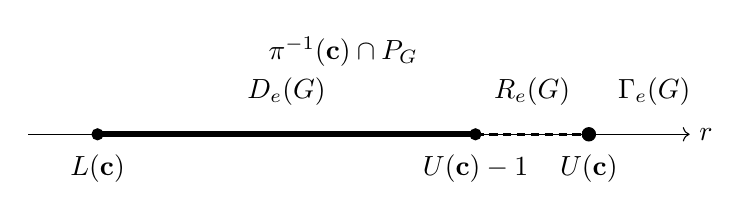
\begin{tikzpicture}[x=1.6cm,y=1cm]
  \draw[->] (0,0) -- (5.25,0) node[right] {$r$};
  \draw[line width=2.2pt] (.55,0) -- (3.55,0);
  \draw[densely dashed,line width=1.2pt] (3.55,0) -- (4.45,0);
  \filldraw (.55,0) circle (2pt);
  \filldraw (3.55,0) circle (2pt);
  \filldraw (4.45,0) circle (2.4pt);
  \node[below=4pt] at (.55,0) {$L(\bc)$};
  \node[below=4pt] at (3.55,0) {$U(\bc)-1$};
  \node[below=4pt] at (4.45,0) {$U(\bc)$};
  \node[above=7pt] at (2.05,0) {$D_e(G)$};
  \node[above=7pt] at (4.0,0) {$R_e(G)$};
  \node[above right=7pt] at (4.45,0) {$\Gamma_e(G)$};
  \node at (2.5,1.05) {$\pi^{-1}(\bc)\cap P_G$};
\end{tikzpicture}
\caption{Schematic geometry of a contraction fiber.  The dashed portion is the
lattice-free residual strip; the upper endpoint represents loopy contraction.}
\label{fig:contraction-fiber}
\end{figure}

\subsection{Geometric parking complexes}
\label{subsec:geometric-parking}

We now iterate the one-step geometry along the same decreasing edge order used
in the deletion-contraction proof of the spanning-forest formula.  At each
deletion step in an intermediate graph $H$,
the child polytope is embedded by the integral-affine translation
\begin{equation}
   \delta_e:P_{H-e}\longrightarrow P_H,
   \qquad \bb\longmapsto \bb+\be_u.
\label{eq:deletion-embedding}
\end{equation}
At each contraction step, the child polytope is embedded by the maximal-lift section
\begin{equation}
   s_e:P_{H/e}\longrightarrow\Gamma_e(H)\subseteq P_H.
\label{eq:contraction-section}
\end{equation}
The first map raises total coordinate sum by one, whereas the second preserves it.

Fix a spanning forest $F$ and follow the corresponding leaf of the deletion-contraction tree.
The edges of $F$ are exactly the edges chosen for
contraction.  A nonforest edge is genuinely deleted unless, when its turn is
reached, its endpoints have already been identified.  Since edges are processed
from largest to smallest, this happens precisely when the edge is externally
active with respect to $F$.
Such an edge has already become a loop and is therefore retained.

So if $T$ is a component of $F$, the vertex corresponding to $T$ in
the terminal loop-only graph carries
\begin{equation}
   m_T=|E(T)|+\eps_F(T)
\label{eq:terminal-loop-number}
\end{equation}
loops.  The score polytope of the terminal graph is the box
\begin{equation}
   \Box_F:=
   \prod_{T\in c(F)}[0,m_T]
   =\prod_{T\in c(F)}
      [0,\,|E(T)|+\eps_F(T)]
   \ \subset\ \RR^{c(F)},
\label{eq:terminal-box}
\end{equation}
its coordinates being indexed by the components of $F$, in accordance with the
convention of Section~\ref{sec:intro}.
Starting from this box and reversing the leaf path, compose the maps
\eqref{eq:deletion-embedding} and~\eqref{eq:contraction-section}.  Once the edge
order and orientations have been fixed, this gives a canonically defined
continuous injective piecewise integral-affine map
\begin{equation}
   \Phi_F:\Box_F\longrightarrow P_G.
\label{eq:parking-map}
\end{equation}
We call its image
\[
   \fC_F:=\Phi_F(\Box_F)
\]
the \emph{geometric parking complex} associated with $F$.  Its lattice points
will be denoted
\begin{equation}  \label{eq:cells}
  C_F:=\fC_F\cap\ZZ^V.
\end{equation}

\begin{theorem}
  [Polyhedral parking cells]
  \label{thm:polyhedral-parking-cells} Fix an ordering and an orientation of the edges of $G$.
For every spanning
forest $F$, the geometric parking complex $\fC_F\subseteq P_G$ has the following properties.
\begin{enumerate}
\item[(i)] The map
\[
   \Phi_F:\Box_F\longrightarrow\fC_F
\]
is a piecewise-linear homeomorphism.  After subdividing $\Box_F$ by
the finitely many domains of linearity of the maximal-lift sections occurring  along the path,
$\fC_F$ is the support of a finite rational polyhedral complex.
On every cell, $\Phi_F$ and its inverse are integral-affine.

\item[(ii)] If $F\ne F'$, then
\begin{equation}
   \fC_F\cap\fC_{F'}=\varnothing.
\label{eq:geometric-cells-disjoint}
\end{equation}

\item[(iii)] The lattice points of the geometric parking complexes give a partition into parking cells~\eqref{eq:cells}
\begin{equation}
   P_G\cap\ZZ^V
   =\bigsqcup_{F\in\cF(G)}C_F.
\label{eq:parking-lattice-partition}
\end{equation}
Moreover $\Phi_F$ restricts to a lattice bijection
\begin{equation}
   \prod_{T\in c(F)}
      \{0,1,\ldots,|E(T)|+\eps_F(T)\}
   \xrightarrow{\ \sim\ } C_F.
\label{eq:parking-chain-product}
\end{equation}

\item[(iv)] Put
\begin{equation}
   d(F):=|E(G)|-|F|-\eps(F),
   \qquad
   \eps(F)=\sum_{T\in c(F)}\eps_F(T).
\label{eq:parking-shift}
\end{equation}
Then for every $x=(x_T)_{T\in c(F)}\in\Box_F$ we have
\begin{equation}
   \sum_{v\in V}(\Phi_F(x))_v  = d(F)+\sum_{T\in c(F)}x_T.
\label{eq:parking-grading}
\end{equation}
Therefore
\begin{equation}
 \sum_{\ba\in C_F}q^{|\ba|} = q^{d(F)} \prod_{T\in c(F)}\left(1+q+\cdots+ q^{|E(T)|+\eps_F(T)}\right).
\label{eq:parking-cell-enumerator}
\end{equation}

\item[(v)] The complement
\begin{equation}
   P_G\setminus\bigcup_{F\in\cF(G)}\fC_F
\label{eq:lattice-free-complement}
\end{equation}
is lattice-free.
\end{enumerate}
\end{theorem}

\begin{proof}
The terminal polytope at the leaf corresponding to $F$ is exactly the box
$\Box_F$.  Reversing the leaf path, every deletion step applies an injective
integral-affine translation, while every contraction applies the injective maximal-lift section of Proposition~\ref{prop:polyhedral-section}.  Thus their
composition $\Phi_F$ is continuous and injective.

Each maximal-lift section is piecewise integral-affine because its upper coordinate
is the minimum of finitely many integral-affine functions, as in~\eqref{eq:U-piecewise-linear}.
Subdivide $\Box_F$ by pulling back all the domains of linearity that occur along the path
and taking their common refinement.
This gives a finite rational polyhedral subdivision on which $\Phi_F$ is integral-affine cell by cell.
Because $\Phi_F$ is globally injective, for any two cells $C_1,C_2$ of this subdivision one has
\[
   \Phi_F(C_1)\cap\Phi_F(C_2)=\Phi_F(C_1\cap C_2).
\]
The intersection $C_1\cap C_2$ is a common face of $C_1$ and $C_2$, and the restrictions
of $\Phi_F$ to the cells are affine bijections.
Hence its image is a common face of $\Phi_F(C_1)$ and $\Phi_F(C_2)$.
The image cells therefore form a finite rational polyhedral complex.
The inverse at each step is either a translation by $-\be_u$ or the integral linear projection $\pi$.
Therefore the inverse on every image cell is integral-affine as well.  This proves (i).

For (ii), take distinct forests $F$ and $F'$ and compare their leaf paths.
Let the first difference occur when a non-loop edge $e$ is processed in some intermediate graph $H$.
One path takes deletion, so at that stage its image is contained in
\[
   D_e(H)=\be_u+P_{H-e},
\]
whereas the other takes contraction, so its image is contained in
$\Gamma_e(H)$.  These two sets are disjoint by
Proposition~\ref{prop:polyhedral-section}(iii).  Up to that stage the two leaf
paths coincide, so the sequence of maps already applied is the same for both.
Therefore the remaining maps carrying the two images back to $P_G$ are
literally the same composition, and it is injective.
An injective map carries disjoint sets to disjoint sets, so the final images $\fC_F$ and $\fC_{F'}$ remain disjoint.

For (iii), every map used in the construction respects the relevant integer
lattices in both directions.  This is immediate for translations.  For a
maximal-lift section it follows from
Proposition~\ref{prop:polyhedral-section}(ii): an integral point of the
contracted polytope has an integral maximal lift, and the inverse projection
sends integral points to integral points.  Hence
\[
   \fC_F\cap\ZZ^V
   =\Phi_F(\Box_F\cap\ZZ^{c(F)}),
\]
and the lattice points of $\Box_F$ are exactly the product in
\eqref{eq:parking-chain-product}.

It remains to see that every lattice point of $P_G$ occurs.  At one
non-loop edge, Proposition~\ref{prop:polyhedral-section}(iii)--(iv) says that
every lattice point belongs to exactly one of the deletion image $D_e(H)$ and
the contraction boundary $\Gamma_e(H)$.  Repeating this decision down the
deletion-contraction tree eventually sends every lattice point to a unique
loop-only leaf.  The leaf is indexed by a unique spanning forest, proving
\eqref{eq:parking-lattice-partition}.

For (iv), a contraction section preserves total coordinate sum, whereas every
genuine deletion translation raises it by one.  Along the leaf associated with
$F$, the contracted edges are the $|F|$ forest edges, and the nonforest edges
that have become loops are precisely the $\eps(F)$ externally active
edges.  Hence the number of genuine deletions is
\[
   |E(G)|-|F|-\eps(F)=d(F).
\]
At the terminal box the total coordinate sum is $\sum_Tx_T$, which proves
\eqref{eq:parking-grading}.  Restricting to the lattice points of the box gives
\eqref{eq:parking-cell-enumerator}.

Finally, (v) follows immediately from (iii): every lattice point of $P_G$ lies
in one of the $\fC_F$, so their complement contains none.
\end{proof}

\begin{remark}\label{rem:not-subdivision}
  Theorem~\ref{thm:polyhedral-parking-cells} upgrades the parking cell partition from a statement about graded finite sets to a genuine polyhedral realization.  It is important, however, not to overstate what the theorem gives.
  The set $\fC_F$ is naturally a piecewise-linearly embedded box and hence the support of a finite rational polyhedral complex. The argument does not show that it is a single convex polytope.
  Moreover, the union of the $\fC_F$ need not be all of $P_G$.  The residual strips from Proposition~\ref{prop:polyhedral-section}(iv), together with their recursive images, may contain real points.
  What is sharp is the lattice statement
\[
 \left(
 P_G\setminus\bigcup_F\fC_F
 \right)\cap\ZZ^V=\varnothing.
\]
Thus the geometric parking complexes give a pairwise disjoint polyhedral realization
of all lattice points of $P_G$, without asserting a subdivision of the whole real polytope.
\end{remark}

\subsection{The Hilbert-series specialization}
\label{subsec:hilbert-specialization}

We can now read the loopy specialization directly from the geometric parking complexes.

\begin{corollary}\label{cor:polytope-specialization}
For every graph $G$,
\begin{equation}
   \sum_{\ba\in P_G\cap\ZZ^V}q^{|\ba|}
   =\LL_G(q,1,1+q,1+q+q^2,\ldots).
\label{eq:polytope-specialization}
\end{equation}
Equivalently,
\[
   \Hil(\BZ_G^e;q)
   =\LL_G(q,1,1+q,1+q+q^2,\ldots).
\]
\end{corollary}

\begin{proof}
By Theorem~\ref{thm:polyhedral-parking-cells},
\begin{align*}
 \sum_{\ba\in P_G\cap\ZZ^V}q^{|\ba|}
 &=\sum_{F\in\cF(G)}
   q^{|E(G)|-|F|-\eps(F)}
   \prod_{T\in c(F)}
   \left(1+q+\cdots+
   q^{|E(T)|+\eps_F(T)}\right).
\end{align*}
By the spanning-forest formula of Theorem~\ref{thm:forests-sum}, the right-hand side is precisely
\[
   \LL_G(q,1,1+q,1+q+q^2,\ldots).
\]
The Hilbert-series statement follows from
\eqref{eq:bizonotopal-lattice-enumerator}.
\end{proof}

\begin{remark}\label{rem:polytope-recursion-check}
The equality in Corollary~\ref{cor:polytope-specialization} also has an
independent verification that does not use the geometric parking complexes.
After the substitution
\[
   t=q,\qquad x_m=1+q+\cdots+q^m,
\]
the loopy recurrence becomes
\[
   H_G(q)=H_{G/e}(q)+qH_{G-e}(q),
\]
with initial value $H_{L_m}(q)=1+q+\cdots+q^m$ on a one-vertex graph with $m$
loops.  These are exactly the external bizonotopal deletion-contraction
relation and initial values of~\cite{KNSV}.  Thus the Hilbert-series identity is
already forced recursively.  The additional content of this section is the
explicit lattice-point partition and, more strongly, its piecewise
integral-affine polyhedral realization.
\end{remark}

Thus the roles of the variables in the loopy polynomial are visible in the geometry.
For a forest component $T$, the variable
$x_{|E(T)|+\eps_F(T)}$ records the interval factor in the terminal box
\eqref{eq:terminal-box}, while the power of $t$ records the genuine deletions,
the edges that are neither forest edges nor externally active ones.


\section{Outlook}\label{sec:outlook}

The results above leave several focused questions.  We list those that seem
most closely tied to the comparison of the loopy and $U$-polynomial
and to the geometry of the score polytope.

\subsection{The equivalence conjecture and the common refinement}
\label{subsec:outlook-equivalence}

The central problem is Conjecture~\ref{conj:L-XB-equivalence}.

\begin{problem}\label{prob:L-vs-U}
  Do $\LL_G$ and $U_G$ distinguish the same simple graphs?  Equivalently,
  is Conjecture~\ref{conj:L-XB-equivalence} true?
\end{problem}

Proposition~\ref{prop:computational-evidence} gives an exhaustive, exact verification
through eleven vertices, but does not explain why the fibers coincide.
Any explanation will have to account for the fact that,
among the three specializations of the common refinement, the loopy polynomial
is distinguished on two grounds: it is the one for which we observed no loss
of distinguishing power on loopless multigraphs
(Section~\ref{subsubsec:multiple-edges}), and its component index is an interval length
in the polyhedral decomposition of $P_G$
(Theorem~\ref{thm:polyhedral-parking-cells}).



We do not know how to connect these two observations, and regard doing so as one of the most promising routes
to Problem~\ref{prob:L-vs-U}.  The common
refinement~\eqref{eq:common-diagram-intro} also suggests a second, asymmetric
question.  Theorem~\ref{thm:MN-solved} solves the Merino--Noble existence problem by
showing that $U^{\ext}\to U$ loses distinguishing power on loopless
multigraphs.  By contrast, no loss was found for $\widehat{\LL}\to\LL$ in
the $48\,229\,871$ connected loopless multigraphs tested.

\begin{problem}\label{prob:extended}
Does
\[
   \LL_G=\LL_H \quad \Longrightarrow\quad  \widehat{\LL}_G=\widehat{\LL}_H
\]
hold for all loopless multigraphs?
More generally, when does $\LL$ determine  $\widehat{\LL}$ if loops are allowed?
\end{problem}

A positive answer for simple graphs would give the implication
$\LL_G=\LL_H\Rightarrow \XB_G=\XB_H$ by
Corollary~\ref{cor:refined-L-determines-XB}.  Two more concrete approaches to
Problem~\ref{prob:L-vs-U} are developed in Section~\ref{sec:tutte-symmetric}:
Problem~\ref{prob:block-transform} isolates the opposite implication, while
Conjecture~\ref{conj:root-injectivity} would settle the connected unicyclic
case by Proposition~\ref{prop:root-injectivity-implies}.  We regard the latter
as the natural rooted-tree problem arising from the present methods, so we do
not duplicate it as a separate Outlook problem.  The analogous bicyclic
analysis, involving two distinguished active components, is a possible next
step once the unicyclic case is understood.

Corollary~\ref{cor:extended-reformulated} suggests a way of accumulating
evidence.  Each invariant that $\widehat{\LL}_G$ is known to determine poses
a weaker question --- is it already determined by $\LL_G$? --- and a positive answer confirms Problem~\ref{prob:extended} on the corresponding piece of $\widehat{\LL}$.
These questions are worth stating because they may be provable one at a time,
and each proved case narrows the room in which a counterexample could live.
They are not, however, a route to a counterexample:
refuting any of them would require a pair of graphs with
equal loopy polynomials and unequal refinements, which is exactly what refuting
Problem~\ref{prob:extended} requires, and the weaker the invariant the more is being asked of such a pair.

Two instances are especially natural.  The first is the generalized degree polynomial.
By Corollary~\ref{cor:gdp}, it is determined by $\widehat{\LL}_G$, and the implication is strict:
the non-isomorphic eight-vertex graphs \texttt{G?qbrg} and \texttt{G?ovdW}, both with twelve
edges and degree sequence $(2,2,3,3,3,3,4,4)$, have the same generalized
degree polynomial but different loopy polynomials.  Thus one may ask the
weaker question whether $\LL_G$ already determines $\GD_G$.  A positive
answer to Problem~\ref{prob:extended} would imply this, while a negative
answer to this weaker question would also give a negative answer to
Problem~\ref{prob:extended}.  In the ranges of
Proposition~\ref{prop:computational-evidence} and
Section~\ref{subsubsec:multiple-edges} the answer is positive, but only
because the $\LL$- and $\widehat{\LL}$-classes coincide there, so these
computations provide no independent evidence for this weaker question.

\begin{problem}\label{prob:L-gdp}
  Does $\LL_G$ determine the generalized degree polynomial $\GD_G$?
\end{problem}


The second instance is the degree sequence of a graph with loops.  By
Theorem~\ref{thm:degree-sequence-loops} it is determined by
$\widehat{\LL}_G$, whereas Theorem~\ref{thm:L-degree-sequence} obtains it
from $\LL_G$ only in the loopless case.  This question seems more
approachable, so we single it out.

\begin{problem}\label{prob:loop-degree}
Does $\LL_G$ determine the degree sequence of an arbitrary graph $G$, loops included?
\end{problem}

\subsection{Complementation, induced statistics, and reconstruction}
\label{subsec:outlook-complementation}

Brylawski's polychromate, and hence $U$ and $\XB$, determines the corresponding
invariant of the complement~\cite{Bry,Nob,Mar}. Proposition~\ref{prop:XB-complement}
makes the $\XB$ transformation explicit.  This motivates a direct loopy question.

\begin{problem}\label{prob:complement}
Does $\LL_G$ determine $\LL_{\overline G}$ for every simple graph $G$?  Is
there a transformation intrinsic to the loopy polynomial?
\end{problem}

The class-level statement follows from Conjecture~\ref{conj:L-XB-equivalence}
and therefore holds through eleven vertices by
Proposition~\ref{prop:computational-evidence}.
Corollary~\ref{cor:independence-clique}(3) gives a direct partial answer:
$\LL_G$ determines the entire induced-edge profile of $\overline G$.

The higher vertex-deletion identity suggests a broader reconstruction question.
It encodes weighted sums of the polynomials $\LL_{G-S}$ and yields
the complete induced edge count profile, but not all induced-subgraph data.
For example, two eight-vertex graphs with the same profile have respectively
$6$ and $8$ induced copies of $P_4$ (graph6 strings
\texttt{GEzvV\char123} and \texttt{GEztv\char123}).  It would be interesting
to determine which symmetric functions of the vertex-deleted collection
$\{\LL_{G-v}:v\in V(G)\}$ are recoverable from $\LL_G$, and whether the loopy
polynomial is reconstructible from a vertex- or edge-deleted deck.

\subsection{Collision statistics}
\label{subsec:outlook-statistics}

The collision data of Section~\ref{sec:extended-U} raise questions independent
of which one of the equivalent invariants is used.  Over the computed range, the
proportion of connected simple graphs in nontrivial classes decreases from
approximately one in $695$ at $n=8$ to one in $22\,366$ at $n=11$.
Does this proportion tend to zero?
Collision classes of size greater than two first occur at ten vertices. Are their sizes bounded?
Complementation and joins generate some larger examples from smaller ones (see  Remark~\ref{rem:complementation}).
It would be useful to identify further operations producing collisions and to understand
to what extent the observed classes are generated from smaller ones.

\subsection{Geometry of the forest pieces}
\label{subsec:outlook-geometry}

Theorem~\ref{thm:polyhedral-parking-cells} realizes every parking cell~\eqref{eq:cells}
as the set of lattice points of a geometric parking complex $\fC_F\subseteq P_G$,
piecewise integral-affinely homeomorphic to the box~\eqref{eq:terminal-box}.
The complexes are pairwise disjoint and their complement is lattice point free, but
the construction does not show that $\fC_F$ are
convex or that their union is all of the real polytope.  Natural questions thus are
whether the residual regions can be assigned recursively
to obtain a subdivision or shelling of $P_G$,
whether  the dependence on the chosen edge order and orientations can be removed, and
whether there is a basis, filtration, or degeneration of the external
bizonotopal algebra whose graded pieces realize the forest factors in
\eqref{eq:parking-cell-enumerator}.

\subsection{Further structural questions}
\label{subsec:outlook-structural}

The normalized loopy polynomial satisfies the same triangular $4$-term
relation as the Tutte symmetric function, although it does not satisfy the
graph $4$-term relation arising from Vassiliev weight systems, see
Remark~\ref{rem:vassiliev-4term}.  It would be useful to understand the
triangular relation conceptually and to determine which specializations,
quotients, or refinements of $\LL$ give genuine graph weight systems.

Finally, since $\LL_G$ is not matroidal, an abstract duality law analogous to
$T_{G^*}(x,y)=T_G(y,x)$ should not be expected without embedding data.  A more
natural direction is a plane- or ribbon-graph refinement of the loopy/common-refinement picture,
perhaps carrying both vertex and face information, for which geometric duality becomes visible.
A dual interpretation of the bizonotopal polytope or of its forest decomposition
on the embedded side would be especially interesting.

\appendix

\section{Computational method}
\label{sec:the-computation}
This section describes how the search reported in
Section~\ref{sec:extended-U} was carried out.
Nothing elsewhere in the paper depends on the details of this computation,
so a reader willing to take Proposition \(\ref{prop:computational-evidence}\) on trust may omit this appendix.

Our computation is organized around the connected-block polynomials $\cC_G(B;q)$
of~\eqref{eq:connected-block-polynomial}, which we compute for all $2^{n}$ vertex subsets
simultaneously by the standard subset recursion
\[
   \cC_G(B;q)
   =
   (1+q)^{e_G(B)}
   -\!\!\sum_{\substack{S\subsetneq B\\ \min B\in S}}\!\!
   \cC_G(S;q)\,(1+q)^{e_G(B\setminus S)},
\]
at a cost of $O(3^{n})$ ring operations.  The three invariants are then read
off as set-partition sums over the blocks: $\XB_G$ by
\eqref{eq:XB-connected-block-expansion}, $\LL_G(1,\bx)$ by
\eqref{eq:L-block-transform}, and $\widehat{\LL}_G$ by the same formula with
the refined block transform, each a further $O(3^{n})$ subset dynamic program.

Evaluating $\LL_G$ and $\widehat{\LL}_G$ appears at first to require the
expansion of $\cC_G(B;q)$ in the basis $q^{s-1}(1+q)^r$, rather than merely
its values.  This expansion can be avoided.  If $s=|B|$, write
\[
  Q_G(B;q)  :=   q^{1-s}\cC_G(B;q)   =   \sum_r a_r(1+q)^r.
\]
The first expression is a polynomial, since $\cC_G(B;q)$ is divisible by $q^{s-1}$.
Hence, for every $\theta$,
\begin{equation}\label{eq:evaluation-trick}
  \sum_r a_r\theta^r   =   Q_G(B;\theta-1).
\end{equation}
Thus any substitution of the form
\[
  u_{s,r}\longmapsto  \sum_{k<K}\beta_{k,s}\theta_k^r
\]
is obtained from $K$ evaluations of the polynomials $Q_G(B;\,\cdot\,)$.
Choosing $\beta_{k,s}=\alpha_k\theta_k^{s-1}$ realizes the diagonal specialization
$u_{s,r}\mapsto x_{s-1+r}$ defining $\LL_G$, while independent random
$\beta_{k,s}$ give random evaluations of $\widehat{\LL}_G$.  The same
$K$ evaluations can therefore be reused for all three invariants,
so computing all three invariants costs little more than computing one.


All arithmetic is carried out in $\FF_p$ with $p=2^{61}-1$, and the substitution points are chosen at random.
We call the resulting tuple of finite-field evaluations the \emph{fingerprint} of the graph.
Because equal polynomials agree under every evaluation, a genuine polynomial collision
necessarily survives the fingerprint stage.  Unequal polynomials may accidentally have
the same finite-field fingerprint, but such false positives are removed at the end by recomputing
every reported class exactly over $\ZZ$.

Two reductions make the range attainable.  First, all three invariants
determine $m(G)$ (Corollary~\ref{th:cor}(4) for $\LL_G$ and the top power of $q$
for $\XB_G$), so collisions occur only within a fixed edge count and the
computation splits into independent jobs, one for each pair $(n,m)$.  Together
with Corollary~\ref{cor:connected-reduction} it suffices to run these on
connected graphs, which we generate with \texttt{geng} from
McKay and Piperno's \texttt{nauty}~\cite{nauty}.  Second, and more
importantly, most graphs can be discarded before any $O(3^{n})$ work is done,
using invariants that $\LL_G$ determines but that are far cheaper to compute.
We apply, in increasing order of cost and each time only to the survivors of the previous stage:
\begin{enumerate}[(i)]
\item $m$, the degree sequence, and the induced edge count profile
  $\bigl(\cE_{G,s}(q)\bigr)_{s}$ of~\eqref{eq:induced-edge-polynomial}, at a cost of $O(2^{n})$
  operations (Theorem~\ref{thm:induced-edge-profile});
\item the number of spanning trees and the number of triangles, $O(n^{3})$ operations (both are determined
  by $T_G$, Corollary~\ref{cor:tutte-specialization});
\item Stanley's chromatic symmetric function $X_G=\XB_G(-1;\bw)$, one further evaluation
  of the block recursion      (Theorem~\ref{thm:L-determines-X}).
\end{enumerate}
Every filter in this list is determined by $\LL_G$, so a graph discarded at any stage
cannot belong to a collision class.  Each is also determined by $\XB_G$,
so the same run computes the collision classes of both invariants.
This sieve substantially reduces the workload: on the complete list of connected
simple graphs with nine vertices, stage~(i) retains $9.2\%$ of the graphs,
stage~(ii) retains $0.18\%$, and stage~(iii) retains $0.058\%$,
so that fewer than one graph in a thousand ever requires the full fingerprints.
Without the sieve the eleven-vertex computation would be roughly an order of magnitude more expensive.

The implementation is in C and is parallelized over graphs.  On an Apple MacBook Pro with an M2 processor
and 16~GB of memory, the complete search takes about $1.5$ minutes for $n=10$
and about $7.5$ hours for $n=11$. The peak memory requirement is roughly $5$~GB,
and is governed by the largest single edge count bucket ($m=27$, some $9.6\times10^{7}$ graphs)
rather than by the total.
The code and the complete lists of colliding graphs are available at~\cite{code}.  As checks
on it we verified that the numbers of connected simple graphs processed agree with
\texttt{A001349}. The fingerprint computation was validated against an independent implementation directly
from the defining expansions on all simple graphs with at most seven vertices.
The whole search was repeated with independent random substitution points, giving identical classes.
For $n\le8$, the collision classes of $\XB_G$ reproduce those found by Markstr\"om~\cite{Mar}
for the $U$-polynomial by an unrelated method.

\medskip

\noindent
\textbf{Acknowledgements.} The third and fourth authors gratefully acknowledge the hospitality
of the Beijing Institute for Mathematical Sciences and Applications during
the initial and the final stages of this project.
%
We used the AI models ChatGPT 5.6 and Claude Opus 5 in the development and drafting of the paper
and in writing the accompanying computer code~\cite{code}.
All statements and proofs were independently checked and are the sole responsibility of the authors.

 \begin{thebibliography}{999}
\bibitem[ACSZ]{ACSZ}
  J.~Aliste-Prieto, L.~Crew, S.~Spirkl, and J.~Zamora,
  A vertex-weighted Tutte symmetric function, and constructing graphs with equal chromatic symmetric function,
  \emph{Electron. J. Combin.} \textbf{28} (2021), no.~2, Paper No.~2.1.

\bibitem[ADZ]{ADZ}
  J.~Aliste-Prieto, A.~de Mier, and J.~Zamora,
  On the smallest trees with the same restricted $U$-polynomial and the
  rooted $U$-polynomial,
  \emph{Discrete Math.} 344 (2021), no.~3, Paper 112255.

\bibitem[AMWZ]{AMWZ}
 J.~Aliste-Prieto, J.~L.~Martin, J.~D.~Wagner, and J.~Zamora,
  Chromatic symmetric functions and polynomial invariants of trees,
  \emph{Bull. London Math. Soc.} 56 (2024), 3452--3476,


\bibitem[AM]{AM}
  D.~Andr\'en and K.~Markstr\"om,
  The bivariate Ising polynomial of a graph,
  \emph{Discrete Appl. Math.} \textbf{157} (2009), no.~11, 2515--2524.

\bibitem[BPR]{BPR}
  B.~Bollob\'as, L.~Pebody, and O.~Riordan,
  Contraction--deletion invariants for graphs,
  \emph{J. Combin. Theory Ser. B} 80 (2000), 320--345.

\bibitem[BR]{BR}
  B.~Bollob\'as and O.~Riordan,
  Polychromatic polynomials,
  \emph{Discrete Math.} 219 (2000), 1--7.

\bibitem[Bry]{Bry}
  T.~H.~Brylawski,
  Intersection theory for graphs,
  \emph{J. Combin. Theory Ser. B} 30 (1981), 233--246.

\bibitem[CDL]{CDL}
  S.~V.~Chmutov, S.~V.~Duzhin, and S.~K.~Lando,
  Vassiliev knot invariants III. Forest algebra and weighted graphs,
  in \emph{Singularities and Bifurcations},
  Adv. Soviet Math. 21, Amer. Math. Soc., Providence, RI, 1994, 135--145.

\bibitem[Cr]{Crew}
  L.~Crew,
  A note on distinguishing trees with the chromatic symmetric function,
  \emph{Discrete Math.} \textbf{345} (2022), no.~8, Paper 112918.

\bibitem[CS1]{CS}
  L.~Crew and S.~Spirkl,
  Modular relations of the Tutte symmetric function,
  \emph{J. Combin. Theory Ser. A} 187 (2022), Paper 105572.

\bibitem[CS2]{CS2}
  L.~Crew and S.~Spirkl,
  A deletion-contraction relation for the chromatic symmetric function,
  \emph{European J. Combin.} \textbf{89} (2020), Paper 103143.


\bibitem[EM]{EM}
J.~Ellis--Monaghan and I.~Moffatt (eds.),
\emph{Handbook of the Tutte Polynomial and Related Topics},
Chapman and Hall/CRC, 2022.

\bibitem[HR]{HR}
O.~Holtz and A.~Ron,
Zonotopal algebra,
\emph{Adv. Math.} 227 (2011), 847--894.

\bibitem[KNSV]{KNSV}
  A.~Kirillov, G.~Nenashev, B.~Shapiro, and A.~Vaintrob,
  Bizonotopal graphical algebras,
  \emph{Algebraic Combinatorics} 9 (2026), no.~3, 831--863.


\bibitem[Code]{code}
  A.~Kirillov, G.~Nenashev, B.~Shapiro, and A.~Vaintrob,
  \emph{loopy-collisions: exhaustive collision search for the loopy   polynomial}, Zenodo (2026),
  \url{https://doi.org/10.5281/zenodo.21929427}.

\bibitem[La]{La}
  S.~K.~Lando,
  On a Hopf algebra in graph theory,
  \emph{J. Combin. Theory Ser. B} 80 (2000), 104--121.

\bibitem[Li]{Li}
  J.~Lieberum,
  Chromatic weight systems and the corresponding knot invariants,
  \emph{Math. Ann.} 317 (2000), 459--482.

\bibitem[Mar]{Mar}
  K.~Markstr\"om,
  From the Ising and Potts models to the general graph homomorphism polynomial,
  in \emph{Graph Polynomials},
  Discrete Math. Appl. (Boca Raton), CRC Press, Boca Raton, FL, 2017, 123--138.


\bibitem[LT]{LT}
  R.~I.~Liu and M.~Tang,
  Generalized degree polynomials of trees,
  \texttt{arXiv:2411.18972}.

\bibitem[McK]{nauty}
  B.~D.~McKay and A.~Piperno,
  Practical graph isomorphism, II,
  \emph{J. Symbolic Comput.} 60 (2014), 94--112.

\bibitem[MM]{MM}
  L.~M.~McDonald and I.~Moffatt,
  On the Potts model partition function in an external field,
  \emph{J. Stat. Phys.} 146 (2012), 1288--1302.

\bibitem[MMN]{MMN}
C.~Merino, A.~de Mier and M.~Noy,
Irreducibility of the Tutte polynomial of a connected matroid,
\emph{J. Combin. Theory Ser. B} 83 (2001), 298--304.

\bibitem[MN]{MN}
  C.~Merino and S.~D.~Noble,
  The equivalence of two graph polynomials and a symmetric function,
  \emph{Combin. Probab. Comput.} 18 (2009), 601--615.

\bibitem[Nob]{Nob}
  S.~D.~Noble,
  The $U$, $V$, and $W$ polynomials,
  in \emph{Handbook of the Tutte Polynomial and Related Topics},
  J.~A.~Ellis-Monaghan and I.~Moffatt (eds.),
  CRC Press, Boca Raton, FL, 2022, 473--496.

\bibitem[NW]{NW}
  S.~D.~Noble and D.~J.~A.~Welsh,
  A weighted graph polynomial from chromatic invariants of knots,
  \emph{Ann. Inst. Fourier (Grenoble)} 49 (1999), 1057--1087.

\bibitem[OS]{OS}
  R.~Orellana and G.~Scott,
  Graphs with equal chromatic symmetric functions,
  \emph{Discrete Math.} 320 (2014), 1--14.

\bibitem[PSS]{PSS}
  A.~Postnikov, B.~Shapiro, and M.~Shapiro,
  Algebras of curvature forms on homogeneous manifolds,
  in \emph{Differential Topology, Infinite-Dimensional Lie Algebras, and Applications},
  Amer. Math. Soc. Transl. Ser.~2, vol.~194, 1999, 227--235.

\bibitem[PS]{PS}
  A.~Postnikov and B.~Shapiro,
  Trees, parking functions, syzygies, and deformations of monomial ideals,
  \emph{Trans. Amer. Math. Soc.} 356 (2004), 3109--3142.

\bibitem[Sar]{Sar}
  I.~Sarmiento,
  The polychromate and a chord diagram polynomial,
  \emph{Ann. Comb.} 4 (2000), no.~2, 227--236.


\bibitem[St1]{Sta}
 R.~P.~Stanley, A symmetric function generalization of the chromatic polynomial of a graph, \emph{Adv. Math.} 111 (1995), 166--194.

\bibitem[St2]{Sta2}
  R.~P.~Stanley, Graph colorings and related symmetric functions: ideas and applications, \emph{Discrete Math.} 193 (1998), 267--286.

\bibitem[Tu1]{Tu1}
  W.~T.~Tutte,
  A ring in graph theory,
  \emph{Proc. Cambridge Philos. Soc.} 43 (1947), 26--40.

\bibitem[Tu2]{Tu2}
  W.~T.~Tutte, A contribution to the theory of chromatic polynomials,
  \emph{Canad. J. Math.} 6 (1954), 80--91.

\bibitem[WS]{WS}
T.~Wang and H.~Sachs,
A contribution to the theory of Tutte's $V$- and $W$-function,
\emph{Discrete Math.} 104 (1992), 281--292.

\end{thebibliography}
\end{document}
